% Annotated study edition of Office Hour Two ("... and Spaces") from
% Clay & Margalit, Office Hours with a Geometric Group Theorist (2017).
% Layout: original page image (left, unchanged) + annotation column (right).
% Build:  tectonic chapter1_annotated.tex
\documentclass[10pt]{article}
\usepackage{fontspec}
\setmainfont{Times New Roman}
\setsansfont{Helvetica Neue}
\usepackage{amsmath,amssymb,amsthm,mathtools}
\usepackage{graphicx}
\usepackage{xcolor}
\usepackage[absolute,overlay]{textpos}
\usepackage{tikz}
\usetikzlibrary{arrows.meta,calc,positioning,shapes.misc,shapes.geometric,decorations.markings,patterns}
\usepackage{tcolorbox}
\tcbuselibrary{skins}
\usepackage{enumitem}
\usepackage{pifont}
\newcommand{\cmark}{\textcolor{why}{\ding{51}}}
\newcommand{\xmark}{\textcolor{pit}{\ding{55}}}
\newcommand{\defterm}[1]{\textbf{\itshape #1}}
\usepackage{array,booktabs}
\usepackage{geometry}
\geometry{paperwidth=11in,paperheight=8.5in,margin=0pt} % US Letter landscape
\pagestyle{empty}
\setlength{\parindent}{0pt}
\setlength{\parskip}{3pt}
\setlength{\TPHorizModule}{1pt}
\setlength{\TPVertModule}{1pt}
\linespread{1.08}

\definecolor{mkc}{RGB}{214,90,0}
\definecolor{why}{RGB}{30,120,60}
\definecolor{pit}{RGB}{180,30,40}
\definecolor{try}{RGB}{160,110,0}
\definecolor{ahead}{RGB}{90,50,160}
\definecolor{big}{RGB}{20,70,150}

\newcommand{\Z}{\mathbb{Z}}
\newcommand{\R}{\mathbb{R}}
\newcommand{\C}{\mathbb{C}}
\newcommand{\GL}{\mathrm{GL}}
\newcommand{\SL}{\mathrm{SL}}
\newcommand{\inv}{^{-1}}

% ---------- marker on the book page ----------
\tikzset{marker/.style={circle,fill=mkc,text=white,font=\sffamily\bfseries\scriptsize,
  inner sep=0pt,minimum size=11pt}}
\newcommand{\mk}[3]{\node[marker] at (#2,#3) {#1};}
\newcommand{\hl}[4]{\fill[yellow,opacity=0.28] (#1,#2) rectangle ++(#3,#4);}
\newcommand{\num}[1]{\tikz[baseline=-3.5pt]\node[marker]{#1};}

% book page: #1 = png suffix (018 ...), #2 = book page number, #3 = marker code
\newcommand{\bookpage}[3]{%
  \begin{textblock*}{380pt}(24pt,20pt)\noindent\includegraphics[height=572pt]{pages/bk-#1.png}\end{textblock*}%
  \begin{textblock*}{380pt}(24pt,20pt)\noindent
    \begin{tikzpicture}[x=0.8602pt,y=-0.8602pt]
      \useasboundingbox (0,0) rectangle (442,665);
      #3
    \end{tikzpicture}
  \end{textblock*}%
  \begin{textblock*}{380pt}(24pt,594pt)\footnotesize\sffamily\color{gray}
    Office Hour 2, book page #2 \hfill annotated study edition\end{textblock*}%
}
% annotation column
\newcommand{\anncol}[1]{%
  \begin{textblock*}{350pt}(418pt,20pt)\small #1\end{textblock*}%
  \mbox{}\clearpage}
% full-width interlude page
\newcommand{\interlude}[2]{%
  \begin{textblock*}{744pt}(24pt,20pt)
    {\sffamily\bfseries\large\color{big} Interlude: #1}\par\vspace{4pt}
    \small #2\end{textblock*}\mbox{}\clearpage}

% ---------- annotation heading ----------
\newcommand{\A}[2]{\par\vspace{4pt}\noindent\num{#1}\ {\sffamily\bfseries #2}\par\nobreak\vspace{1pt}}

% ---------- boxes ----------
\newtcolorbox{why}{enhanced,colback=why!5,colframe=why,boxrule=0.5pt,arc=2pt,
  left=4pt,right=4pt,top=2pt,bottom=2pt,boxsep=1pt,fontupper=\small,
  title={\sffamily\bfseries Why?},fonttitle=\scriptsize,coltitle=white,colbacktitle=why,
  attach boxed title to top left={xshift=4pt,yshift=-2pt},boxed title style={size=small,arc=1pt,boxrule=0pt}}
\newtcolorbox{pitfall}{enhanced,colback=pit!5,colframe=pit,boxrule=0.5pt,arc=2pt,
  left=4pt,right=4pt,top=2pt,bottom=2pt,boxsep=1pt,fontupper=\small,
  title={\sffamily\bfseries Watch out},fonttitle=\scriptsize,coltitle=white,colbacktitle=pit,
  attach boxed title to top left={xshift=4pt,yshift=-2pt},boxed title style={size=small,arc=1pt,boxrule=0pt}}
\newtcolorbox{tryit}{enhanced,colback=try!6,colframe=try,boxrule=0.5pt,arc=2pt,
  left=4pt,right=4pt,top=2pt,bottom=2pt,boxsep=1pt,fontupper=\small,
  title={\sffamily\bfseries Try it},fonttitle=\scriptsize,coltitle=white,colbacktitle=try,
  attach boxed title to top left={xshift=4pt,yshift=-2pt},boxed title style={size=small,arc=1pt,boxrule=0pt}}
\newtcolorbox{lookahead}{enhanced,colback=ahead!5,colframe=ahead,boxrule=0.5pt,arc=2pt,
  left=4pt,right=4pt,top=2pt,bottom=2pt,boxsep=1pt,fontupper=\small,
  title={\sffamily\bfseries Looking ahead},fonttitle=\scriptsize,coltitle=white,colbacktitle=ahead,
  attach boxed title to top left={xshift=4pt,yshift=-2pt},boxed title style={size=small,arc=1pt,boxrule=0pt}}
\newtcolorbox{bigpic}{enhanced,colback=big!5,colframe=big,boxrule=0.5pt,arc=2pt,
  left=4pt,right=4pt,top=2pt,bottom=2pt,boxsep=1pt,fontupper=\small,
  title={\sffamily\bfseries Big picture},fonttitle=\scriptsize,coltitle=white,colbacktitle=big,
  attach boxed title to top left={xshift=4pt,yshift=-2pt},boxed title style={size=small,arc=1pt,boxrule=0pt}}
\newtcolorbox{prereq}{enhanced,colback=gray!8,colframe=gray!60!black,boxrule=0.5pt,arc=2pt,
  left=4pt,right=4pt,top=2pt,bottom=2pt,boxsep=1pt,fontupper=\small,
  title={\sffamily\bfseries Background you need},fonttitle=\scriptsize,coltitle=white,colbacktitle=gray!60!black,
  attach boxed title to top left={xshift=4pt,yshift=-2pt},boxed title style={size=small,arc=1pt,boxrule=0pt}}

% =====================================================================
%                              FIGURES
% =====================================================================
\newcommand{\figtriangle}{%
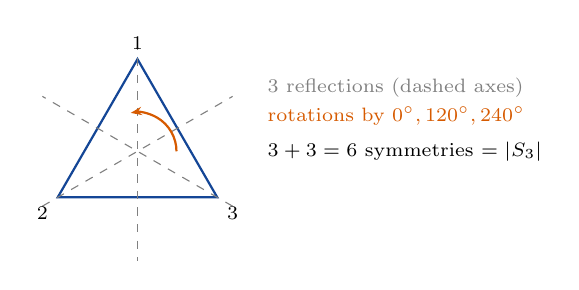
\begin{tikzpicture}[scale=0.9]
  \coordinate (A) at (90:1.3); \coordinate (B) at (210:1.3); \coordinate (C) at (330:1.3);
  \draw[thick,big] (A)--(B)--(C)--cycle;
  \foreach \ang in {90,210,330} \draw[dashed,gray] (\ang:1.55) -- (\ang+180:1.55);
  \draw[-{Stealth[length=4pt]},mkc,thick] (0.55,0) arc (0:100:0.55);
  \node[font=\scriptsize] at (A) [above] {1}; \node[font=\scriptsize] at (B) [below left] {2}; \node[font=\scriptsize] at (C) [below right] {3};
  \node[font=\scriptsize,text=gray,anchor=west] at (1.7,0.9) {3 reflections (dashed axes)};
  \node[font=\scriptsize,text=mkc,anchor=west] at (1.7,0.5) {rotations by $0^\circ,120^\circ,240^\circ$};
  \node[font=\scriptsize,anchor=west] at (1.7,0.0) {$3+3=6$ symmetries $=|S_3|$};
\end{tikzpicture}}

\newcommand{\figcube}[1]{%
\begin{tikzpicture}[scale=#1,line join=round]
  \coordinate (A) at (0,0); \coordinate (B) at (3,0); \coordinate (C) at (3,3); \coordinate (D) at (0,3);
  \coordinate (E) at (1.3,1.3); \coordinate (F) at (4.3,1.3); \coordinate (G) at (4.3,4.3); \coordinate (H) at (1.3,4.3);
  \draw[thick] (A)--(B)--(C)--(D)--cycle;
  \draw[thick] (B)--(F)--(G)--(C); \draw[thick] (D)--(H)--(G);
  \draw[thick,dashed,gray] (A)--(E)--(F); \draw[thick,dashed,gray] (E)--(H);
  \draw[very thick,red!80!black] (A)--(G);
  \draw[very thick,blue!70!black] (B)--(H);
  \draw[very thick,green!55!black] (C)--(E);
  \draw[very thick,orange!90!black] (D)--(F);
  \foreach \p/\l/\pos in {A/A/below left,B/B/below right,C/C/above right,D/D/above left,E/E/left,F/F/right,G/G/above right,H/H/above left}
    \node[font=\scriptsize,\pos] at (\p) {$\l$};
  \node[font=\scriptsize,red!80!black] at (2.6,2.9) {$d_1$};
  \node[font=\scriptsize,blue!70!black] at (1.7,1.55) {$d_2$};
  \node[font=\scriptsize,green!55!black] at (2.35,2.1) {$d_3$};
  \node[font=\scriptsize,orange!90!black] at (2.9,1.3) {$d_4$};
\end{tikzpicture}}

\newcommand{\figpent}{%
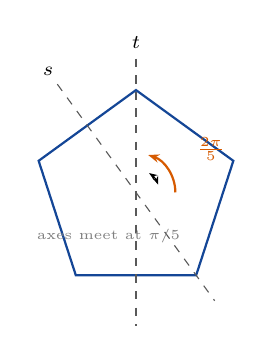
\begin{tikzpicture}[scale=1.0]
  \foreach \k in {0,...,4} \coordinate (P\k) at ({90+72*\k}:1.3);
  \draw[thick,big] (P0)--(P1)--(P2)--(P3)--(P4)--cycle;
  \draw[dashed,gray!70!black] (90:1.7)--(270:1.7);
  \draw[dashed,gray!70!black] (126:1.7)--(306:1.7);
  \node[font=\scriptsize] at (90:1.9) {$t$};
  \node[font=\scriptsize] at (126:1.9) {$s$};
  \draw[-{Stealth[length=4pt]},mkc,thick] (0.5,0) arc (0:72:0.5);
  \node[font=\scriptsize,mkc] at (0.95,0.55) {$\tfrac{2\pi}{5}$};
  \draw[{Stealth[length=3pt]}-{Stealth[length=3pt]},thin] (0.28,0.1) arc (20:56:0.3);
  \node[font=\tiny,gray] at (-0.35,-0.55) {axes meet at $\pi/5$};
\end{tikzpicture}}

\newcommand{\figcompose}{%
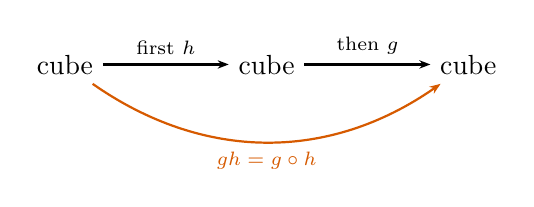
\begin{tikzpicture}[node distance=1.6cm,>={Stealth[length=4pt]}]
  \node (x) {cube};
  \node (y) [right=of x] {cube};
  \node (z) [right=of y] {cube};
  \draw[->,thick] (x) -- node[above,font=\scriptsize] {first $h$} (y);
  \draw[->,thick] (y) -- node[above,font=\scriptsize] {then $g$} (z);
  \draw[->,thick,mkc] (x) to[bend right=35] node[below,font=\scriptsize] {$gh=g\circ h$} (z);
\end{tikzpicture}}

\newcommand{\figbraid}{%
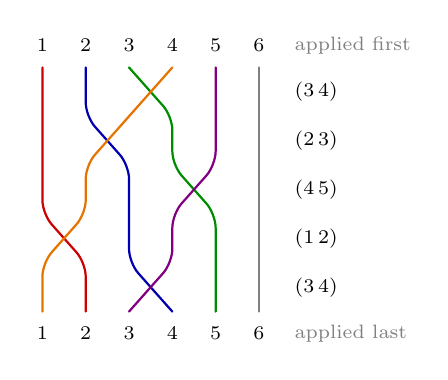
\begin{tikzpicture}[x=0.55cm,y=0.62cm,line cap=round]
  \foreach \i in {1,...,6} {\node[font=\scriptsize] at (\i,0.45) {\i}; \node[font=\scriptsize] at (\i,-5.45) {\i};}
  \draw[thick,red!80!black,rounded corners=5pt] (1,0)--(1,-1)--(1,-2)--(1,-3)--(2,-4)--(2,-5);
  \draw[thick,blue!70!black,rounded corners=5pt] (2,0)--(2,-1)--(3,-2)--(3,-3)--(3,-4)--(4,-5);
  \draw[thick,green!55!black,rounded corners=5pt] (3,0)--(4,-1)--(4,-2)--(5,-3)--(5,-4)--(5,-5);
  \draw[thick,orange!90!black,rounded corners=5pt] (4,0)--(3,-1)--(2,-2)--(2,-3)--(1,-4)--(1,-5);
  \draw[thick,violet,rounded corners=5pt] (5,0)--(5,-1)--(5,-2)--(4,-3)--(4,-4)--(3,-5);
  \draw[thick,gray] (6,0)--(6,-5);
  \foreach \y/\l in {0.5/(3\,4), 1.5/(2\,3), 2.5/(4\,5), 3.5/(1\,2), 4.5/(3\,4)}
    \node[font=\scriptsize,anchor=west] at (6.6,-\y) {$\l$};
  \node[font=\scriptsize,anchor=west,gray] at (6.6,0.45) {applied first};
  \node[font=\scriptsize,anchor=west,gray] at (6.6,-5.45) {applied last};
\end{tikzpicture}}

\newcommand{\figstack}{%
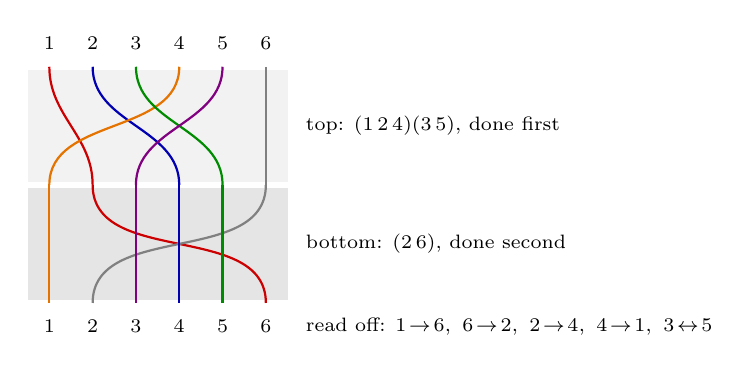
\begin{tikzpicture}[x=0.55cm,y=0.75cm]
  \foreach \i in {1,...,6} {\node[font=\scriptsize] at (\i,0.4) {\i}; \node[font=\scriptsize] at (\i,-4.4) {\i};}
  \fill[gray!10] (0.5,-0.05) rectangle (6.5,-1.95);
  \fill[gray!20] (0.5,-2.05) rectangle (6.5,-3.95);
  % top block: (1 2 4)(3 5): i -> sigma(i)
  \foreach \a/\b/\c in {1/2/red!80!black, 2/4/blue!70!black, 4/1/orange!90!black, 3/5/green!55!black, 5/3/violet, 6/6/gray}
    \draw[thick,\c] (\a,0) to[out=-90,in=90] (\b,-2);
  % bottom block: (2 6)
  \foreach \a/\b/\c in {2/6/red!80!black, 6/2/gray, 1/1/orange!90!black, 3/3/violet, 4/4/blue!70!black, 5/5/green!55!black}
    \draw[thick,\c] (\a,-2) to[out=-90,in=90] (\b,-4);
  \node[font=\scriptsize,anchor=west] at (6.7,-1) {top: $(1\,2\,4)(3\,5)$, done first};
  \node[font=\scriptsize,anchor=west] at (6.7,-3) {bottom: $(2\,6)$, done second};
  \node[font=\scriptsize,anchor=west] at (6.7,-4.4) {read off: $1\!\to\!6,\ 6\!\to\!2,\ 2\!\to\!4,\ 4\!\to\!1,\ 3\!\leftrightarrow\!5$};
\end{tikzpicture}}

\newcommand{\figclock}{%
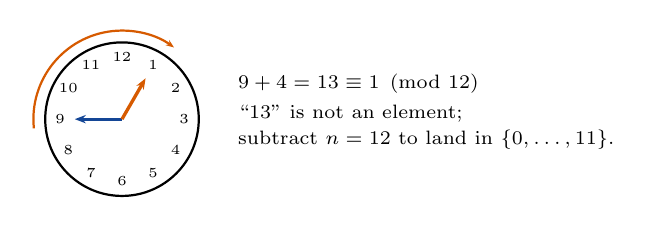
\begin{tikzpicture}[scale=0.75]
  \draw[thick] (0,0) circle (1.3);
  \foreach \h in {1,...,12} \node[font=\tiny] at ({90-30*\h}:1.05) {\h};
  \draw[-{Stealth[length=4pt]},very thick,big] (0,0) -- ({90-30*9}:0.8);
  \draw[-{Stealth[length=4pt]},very thick,mkc] (0,0) -- ({90-30*1}:0.8);
  \draw[-{Stealth[length=3pt]},mkc,thick] ({90-30*9+6}:1.5) arc ({90-30*9+6}:{90-30*13-6}:1.5);
  \node[font=\scriptsize,anchor=west] at (1.8,0.6) {$9+4=13\equiv 1 \pmod{12}$};
  \node[font=\scriptsize,anchor=west] at (1.8,0.1) {``$13$'' is not an element;};
  \node[font=\scriptsize,anchor=west] at (1.8,-0.35) {subtract $n=12$ to land in $\{0,\dots,11\}$.};
\end{tikzpicture}}

\newcommand{\figarrowgon}{%
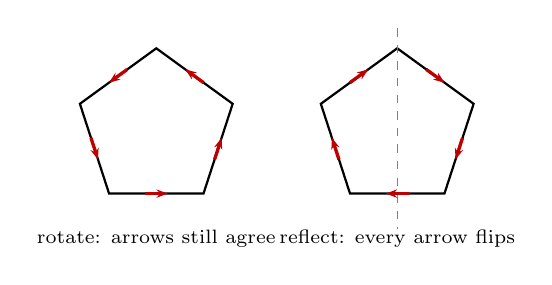
\begin{tikzpicture}[scale=0.85]
  \begin{scope}
    \foreach \k in {0,...,4} \coordinate (P\k) at ({90+72*\k}:1.2);
    \draw[thick] (P0)--(P1)--(P2)--(P3)--(P4)--cycle;
    \foreach \k in {0,...,4} {\pgfmathtruncatemacro{\nk}{mod(\k+1,5)}
      \draw[-{Stealth[length=4pt]},very thick,red!75!black] ($(P\k)!0.38!(P\nk)$)--($(P\k)!0.62!(P\nk)$);}
    \node[font=\scriptsize] at (0,-1.65) {rotate: arrows still agree};
  \end{scope}
  \begin{scope}[xshift=3.6cm]
    \foreach \k in {0,...,4} \coordinate (Q\k) at ({90-72*\k}:1.2);
    \draw[thick] (Q0)--(Q1)--(Q2)--(Q3)--(Q4)--cycle;
    \draw[dashed,gray] (0,1.5)--(0,-1.5);
    \foreach \k in {0,...,4} {\pgfmathtruncatemacro{\nk}{mod(\k+1,5)}
      \draw[-{Stealth[length=4pt]},very thick,red!75!black] ($(Q\k)!0.38!(Q\nk)$)--($(Q\k)!0.62!(Q\nk)$);}
    \node[font=\scriptsize] at (0,-1.65) {reflect: every arrow flips};
  \end{scope}
\end{tikzpicture}}

\newcommand{\figline}{%
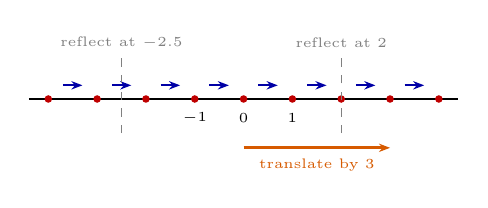
\begin{tikzpicture}[scale=0.62]
  \draw[thick] (-4.4,0)--(4.4,0);
  \foreach \x in {-4,...,4} \fill[red!75!black] (\x,0) circle (2.2pt);
  \foreach \x in {-4,...,3} \draw[-{Stealth[length=4pt]},thick,blue!65!black] (\x+0.3,0.28)--(\x+0.7,0.28);
  \node[font=\tiny] at (0,-0.4) {0}; \node[font=\tiny] at (1,-0.4) {1}; \node[font=\tiny] at (-1,-0.4) {$-1$};
  \draw[dashed,gray] (2,-0.7)--(2,0.9); \node[font=\tiny,gray] at (2,1.15) {reflect at 2};
  \draw[dashed,gray] (-2.5,-0.7)--(-2.5,0.9); \node[font=\tiny,gray] at (-2.5,1.15) {reflect at $-2.5$};
  \draw[-{Stealth[length=4pt]},very thick,mkc] (0,-1.0) -- (3,-1.0); \node[font=\tiny,mkc] at (1.5,-1.35) {translate by $3$};
\end{tikzpicture}}

\newcommand{\figlattice}{%
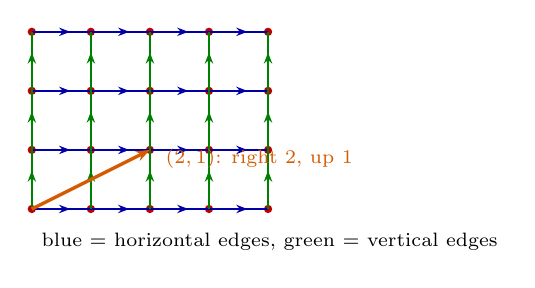
\begin{tikzpicture}[scale=0.75]
  \foreach \x in {0,...,4} \foreach \y in {0,...,3} \fill[red!75!black] (\x,\y) circle (2pt);
  \foreach \y in {0,...,3} \foreach \x in {0,...,3} {
    \draw[blue!65!black,thick] (\x,\y)--(\x+1,\y);
    \draw[-{Stealth[length=4pt]},blue!65!black,thick] (\x+0.35,\y)--(\x+0.65,\y);}
  \foreach \x in {0,...,4} \foreach \y in {0,...,2} {
    \draw[green!50!black,thick] (\x,\y)--(\x,\y+1);
    \draw[-{Stealth[length=4pt]},green!50!black,thick] (\x,\y+0.35)--(\x,\y+0.65);}
  \draw[-{Stealth[length=5pt]},very thick,mkc] (0,0)--(2,1);
  \node[font=\scriptsize,mkc,anchor=west] at (2.1,0.85) {$(2,1)$: right 2, up 1};
  \node[font=\scriptsize,anchor=north west] at (0,-0.25) {blue = horizontal edges, green = vertical edges};
\end{tikzpicture}}

\newcommand{\figreduce}{%
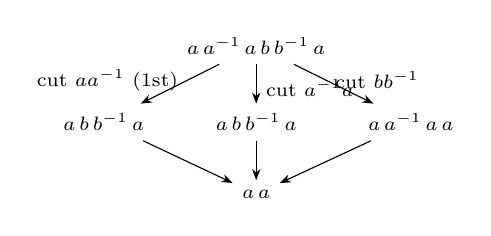
\begin{tikzpicture}[node distance=5mm and 3mm,>={Stealth[length=4pt]},every node/.style={font=\scriptsize}]
  \node (w) {$a\,a\inv\,a\,b\,b\inv\,a$};
  \node (l) [below left=of w] {$a\,b\,b\inv\,a$};
  \node (m) [below=of w] {$a\,b\,b\inv\,a$};
  \node (r) [below right=of w] {$a\,a\inv\,a\,a$};
  \node (e) [below=of m] {$a\,a$};
  \draw[->] (w) -- node[left,pos=0.4] {cut $a a\inv$ (1st)} (l);
  \draw[->] (w) -- node[right,pos=0.6] {cut $a\inv a$} (m);
  \draw[->] (w) -- node[right,pos=0.4] {cut $b b\inv$} (r);
  \draw[->] (l) -- (e); \draw[->] (m) -- (e); \draw[->] (r) -- (e);
\end{tikzpicture}}

\newcommand{\figtree}{%
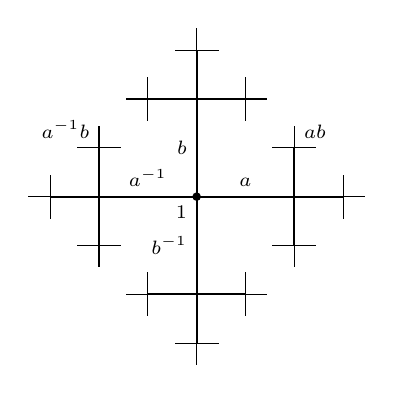
\begin{tikzpicture}[scale=0.62]
  \foreach \d/\o in {0/180,90/270,180/0,270/90} {
    \draw[thick] (0,0) -- (\d:2);
    \foreach \e in {0,90,180,270} {
      \ifnum\e=\o\relax\else
        \draw[thick] (\d:2) -- ($(\d:2)+(\e:1)$);
        \pgfmathtruncatemacro{\eo}{mod(\e+180,360)}
        \foreach \f in {0,90,180,270} {
          \ifnum\f=\eo\relax\else
            \draw[thin] ($(\d:2)+(\e:1)$) -- ($(\d:2)+(\e:1)+(\f:0.45)$);
          \fi }
      \fi } }
  \fill (0,0) circle (2.5pt);
  \node[font=\scriptsize,above] at (1,0) {$a$};
  \node[font=\scriptsize,left] at (0,1) {$b$};
  \node[font=\scriptsize,above] at (-1,0) {$a\inv$};
  \node[font=\scriptsize,left] at (0,-1) {$b\inv$};
  \node[font=\scriptsize,below left] at (0,0) {$1$};
  \node[font=\scriptsize,above right] at (2,1) {$ab$};
  \node[font=\scriptsize,above left] at (-2,1) {$a\inv b$};
\end{tikzpicture}}

\newcommand{\fighom}{%
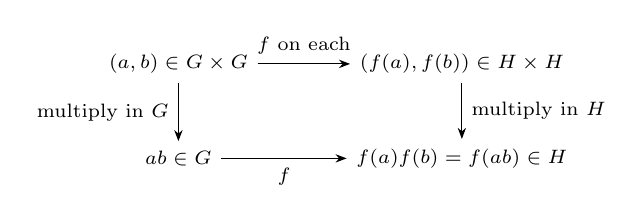
\begin{tikzpicture}[>={Stealth[length=4pt]},every node/.style={font=\scriptsize}]
  \node (a) at (0,1.2) {$(a,b)\in G\times G$};
  \node (b) at (3.6,1.2) {$(f(a),f(b))\in H\times H$};
  \node (c) at (0,0) {$ab\in G$};
  \node (d) at (3.6,0) {$f(a)f(b)=f(ab)\in H$};
  \draw[->] (a) -- node[above] {$f$ on each} (b);
  \draw[->] (a) -- node[left] {multiply in $G$} (c);
  \draw[->] (b) -- node[right] {multiply in $H$} (d);
  \draw[->] (c) -- node[below] {$f$} (d);
\end{tikzpicture}}

\newcommand{\figwrap}{%
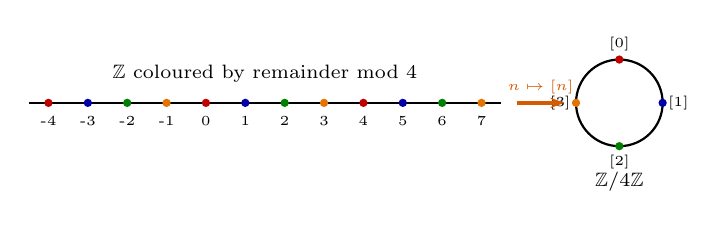
\begin{tikzpicture}[scale=0.5]
  \draw[thick] (-4.5,0)--(7.5,0);
  \foreach \x in {-4,...,7} {\pgfmathtruncatemacro{\r}{mod(\x+8,4)}
    \ifnum\r=0 \fill[red!75!black] (\x,0) circle (3pt);\fi
    \ifnum\r=1 \fill[blue!65!black] (\x,0) circle (3pt);\fi
    \ifnum\r=2 \fill[green!50!black] (\x,0) circle (3pt);\fi
    \ifnum\r=3 \fill[orange!90!black] (\x,0) circle (3pt);\fi
    \node[font=\tiny] at (\x,-0.45) {\x};}
  \node[font=\scriptsize] at (1.5,0.75) {$\Z$ coloured by remainder mod 4};
  \begin{scope}[xshift=10.5cm]
    \draw[thick] (0,0) circle (1.1);
    \fill[red!75!black] (90:1.1) circle (3pt); \node[font=\tiny] at (90:1.5) {$[0]$};
    \fill[blue!65!black] (0:1.1) circle (3pt); \node[font=\tiny] at (0:1.5) {$[1]$};
    \fill[green!50!black] (270:1.1) circle (3pt); \node[font=\tiny] at (270:1.5) {$[2]$};
    \fill[orange!90!black] (180:1.1) circle (3pt); \node[font=\tiny] at (180:1.5) {$[3]$};
    \node[font=\scriptsize] at (0,-2.0) {$\Z/4\Z$};
  \end{scope}
  \draw[-{Stealth[length=5pt]},very thick,mkc] (7.9,0) -- (9.1,0); \node[font=\tiny,mkc] at (8.5,0.4) {$n\mapsto[n]$};
\end{tikzpicture}}

\newcommand{\figiso}{%
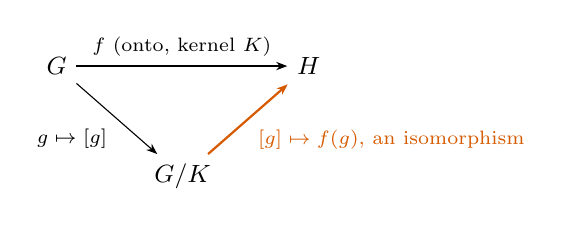
\begin{tikzpicture}[>={Stealth[length=4pt]},every node/.style={font=\small}]
  \node (G) at (0,1.4) {$G$};
  \node (H) at (3.2,1.4) {$H$};
  \node (Q) at (1.6,0) {$G/K$};
  \draw[->] (G) -- node[above,font=\scriptsize] {$f$ (onto, kernel $K$)} (H);
  \draw[->] (G) -- node[below left,font=\scriptsize] {$g\mapsto[g]$} (Q);
  \draw[->,mkc,thick] (Q) -- node[below right,font=\scriptsize] {$[g]\mapsto f(g)$, an isomorphism} (H);
\end{tikzpicture}}

\newcommand{\figpres}{%
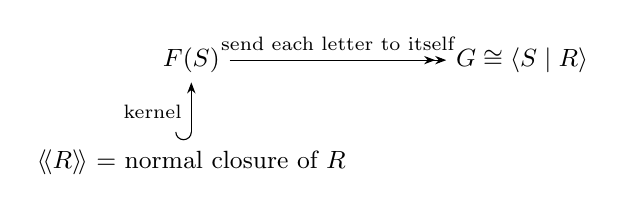
\begin{tikzpicture}[>={Stealth[length=4pt]},every node/.style={font=\small}]
  \node (F) at (0,0) {$F(S)$};
  \node (G) at (4.2,0) {$G\cong\langle S\mid R\rangle$};
  \node (N) at (0,-1.3) {$\langle\!\langle R\rangle\!\rangle$ = normal closure of $R$};
  \draw[-{Stealth[length=4pt]Stealth[length=4pt]}] (F) -- node[above,font=\scriptsize] {send each letter to itself} (G);
  \draw[{Hooks[right,length=3pt]}-{Stealth[length=4pt]}] (N) -- node[left,font=\scriptsize] {kernel} (F);
\end{tikzpicture}}

\newcommand{\figmap}{%
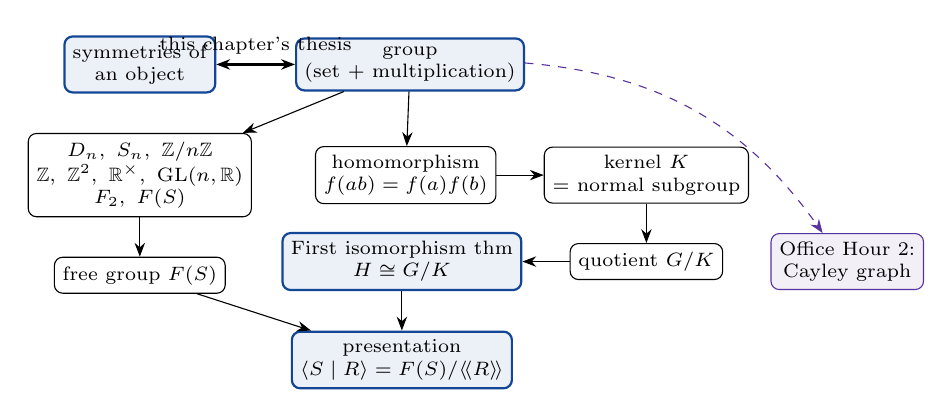
\begin{tikzpicture}[>={Stealth[length=5pt]},node distance=5mm and 6mm,
  box/.style={draw,rounded corners=3pt,align=center,font=\scriptsize,inner sep=3pt,fill=white},
  key/.style={box,fill=big!8,draw=big,thick}]
  \node[key] (sym) {symmetries of\\an object};
  \node[key,right=10mm of sym] (grp) {group\\(set + multiplication)};
  \node[box,below=of sym] (ex) {$D_n,\ S_n,\ \Z/n\Z$\\$\Z,\ \Z^2,\ \R^\times,\ \GL(n,\R)$\\$F_2,\ F(S)$};
  \node[box,right=8mm of ex] (hom) {homomorphism\\$f(ab)=f(a)f(b)$};
  \node[box,right=of hom] (ker) {kernel $K$\\= normal subgroup};
  \node[box,below=of ker] (quo) {quotient $G/K$};
  \node[key,left=of quo] (iso) {First isomorphism thm\\$H\cong G/K$};
  \node[box,below=of ex] (free) {free group $F(S)$};
  \node[key,below=of iso] (pres) {presentation\\$\langle S\mid R\rangle = F(S)/\langle\!\langle R\rangle\!\rangle$};
  \node[box,right=of quo,fill=ahead!8,draw=ahead] (cay) {Office Hour 2:\\Cayley graph};
  \draw[<->,thick] (sym) -- node[above,font=\scriptsize] {this chapter's thesis} (grp);
  \draw[->] (grp) -- (ex); \draw[->] (grp) -- (hom); \draw[->] (hom) -- (ker); \draw[->] (ker) -- (quo);
  \draw[->] (quo) -- (iso); \draw[->] (ex) -- (free); \draw[->] (free) -- (pres); \draw[->] (iso) -- (pres);
  \draw[->,ahead,dashed] (grp) to[bend left=25] (cay);
\end{tikzpicture}}

% ---------------- extra visualisations ----------------
% gallery of the 8 symmetries of a square; #1..#4 = labels at TL,TR,BR,BL; #5 caption; #6 axis code
\newcommand{\sq}[6]{%
\begin{tikzpicture}[scale=0.55]
  \draw[thick,big] (0,0) rectangle (2,2);
  #6
  \node[font=\scriptsize] at (0.25,1.75) {#1}; \node[font=\scriptsize] at (1.75,1.75) {#2};
  \node[font=\scriptsize] at (1.75,0.25) {#3}; \node[font=\scriptsize] at (0.25,0.25) {#4};
  \node[font=\scriptsize,align=center] at (1,-0.55) {#5};
\end{tikzpicture}}
\newcommand{\figsquares}{%
\begin{tabular}{@{}cccc@{}}
\sq{1}{2}{3}{4}{identity $1$}{} &
\sq{2}{3}{4}{1}{$r$ = turn $90^\circ$}{\draw[-{Stealth[length=3pt]},mkc,thick] (1.45,1) arc (0:270:0.45);} &
\sq{3}{4}{1}{2}{$r^2$}{\draw[-{Stealth[length=3pt]},mkc,thick] (1.45,1) arc (0:180:0.45);} &
\sq{4}{1}{2}{3}{$r^3$}{\draw[-{Stealth[length=3pt]},mkc,thick] (1.45,1) arc (0:90:0.45);}\\[2pt]
\sq{2}{1}{4}{3}{$s$ (vertical axis)}{\draw[dashed,pit] (1,-0.2)--(1,2.2);} &
\sq{4}{3}{2}{1}{$sr^2$ (horizontal)}{\draw[dashed,pit] (-0.2,1)--(2.2,1);} &
\sq{1}{4}{3}{2}{$sr$ (diagonal)}{\draw[dashed,pit] (-0.2,2.2)--(2.2,-0.2);} &
\sq{3}{2}{1}{4}{$sr^3$ (other diagonal)}{\draw[dashed,pit] (-0.2,-0.2)--(2.2,2.2);}\\
\end{tabular}}

\newcommand{\figcayleytable}{%
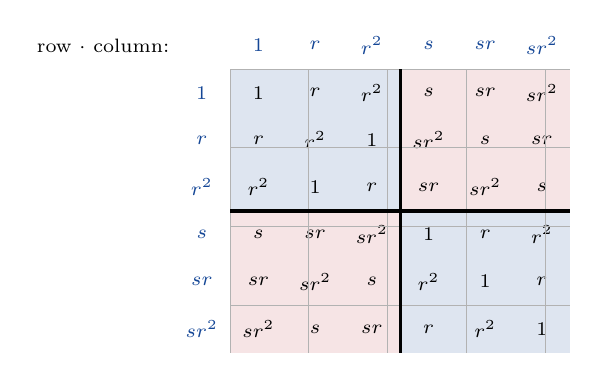
\begin{tikzpicture}[x=0.72cm,y=-0.6cm]
  \def\els{{"$1$","$r$","$r^2$","$s$","$sr$","$sr^2$"}}
  % table body: 1=rotation, 2=reflection; entries as strings
  \foreach \i/\row in {0/{1,r,r^2,s,sr,sr^2}, 1/{r,r^2,1,sr^2,s,sr}, 2/{r^2,1,r,sr,sr^2,s}, 3/{s,sr,sr^2,1,r,r^2}, 4/{sr,sr^2,s,r^2,1,r}, 5/{sr^2,s,sr,r,r^2,1}} {
    \foreach \e [count=\j from 0] in \row {
      \pgfmathtruncatemacro{\isrot}{ifthenelse(\j<3,1,0)*ifthenelse(\i<3,1,0)+ifthenelse(\j>2,1,0)*ifthenelse(\i>2,1,0)}
      \ifnum\isrot=1 \fill[big!14] (\j,\i) rectangle ++(1,1); \else \fill[pit!12] (\j,\i) rectangle ++(1,1); \fi
      \node[font=\scriptsize] at (\j+0.5,\i+0.5) {$\e$};
    } }
  \draw[gray!60] (0,0) grid (6,6);
  \draw[very thick] (3,0)--(3,6); \draw[very thick] (0,3)--(6,3);
  \foreach \e [count=\j from 0] in {1,r,r^2,s,sr,sr^2} {\node[font=\scriptsize,big] at (\j+0.5,-0.5) {$\e$}; \node[font=\scriptsize,big] at (-0.5,\j+0.5) {$\e$};}
  \node[font=\scriptsize,anchor=east] at (-0.9,-0.5) {row $\cdot$ column:};
\end{tikzpicture}}

\newcommand{\figaxes}{%
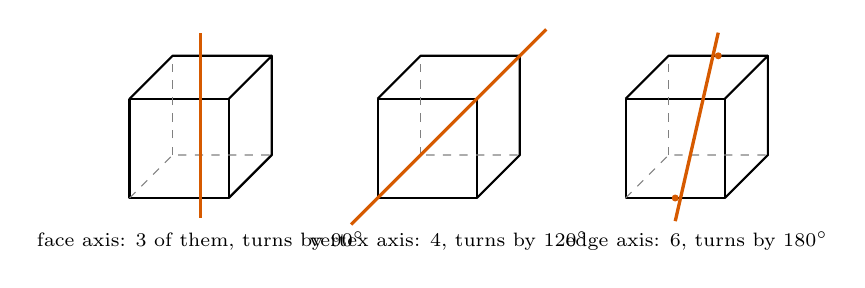
\begin{tikzpicture}[scale=0.42,line join=round]
  \foreach \dx/\axis/\cap in {0/face/{face axis: 3 of them, turns by $90^\circ$}, 7.5/vertex/{vertex axis: 4, turns by $120^\circ$}, 15/edge/{edge axis: 6, turns by $180^\circ$}} {
    \begin{scope}[xshift=\dx cm]
      \coordinate (A) at (0,0); \coordinate (B) at (3,0); \coordinate (C) at (3,3); \coordinate (D) at (0,3);
      \coordinate (E) at (1.3,1.3); \coordinate (F) at (4.3,1.3); \coordinate (G) at (4.3,4.3); \coordinate (H) at (1.3,4.3);
      \draw[thick] (A)--(B)--(C)--(D)--cycle; \draw[thick] (B)--(F)--(G)--(C); \draw[thick] (D)--(H)--(G);
      \draw[dashed,gray] (A)--(E)--(F); \draw[dashed,gray] (E)--(H);
      \node[font=\scriptsize,align=center] at (2.15,-1.3) {\cap};
    \end{scope} }
  \draw[very thick,mkc] (2.15,-0.6) -- (2.15,5.0);
  \draw[very thick,mkc] (7.5-0.8,-0.8) -- (7.5+4.3+0.8,4.3+0.8);
  \draw[very thick,mkc] (15+1.5,-0.7) -- (15+2.8,5.0);
  \fill[mkc] (15+1.5,0) circle (3pt); \fill[mkc] (15+2.8,4.3) circle (3pt);
\end{tikzpicture}}

\newcommand{\figcyclearrows}{%
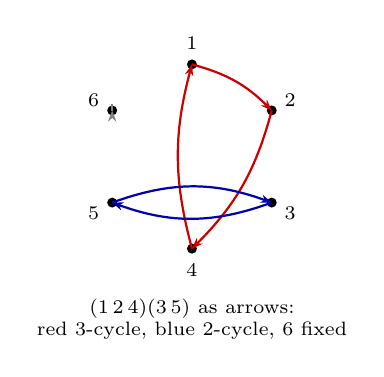
\begin{tikzpicture}[scale=0.9,>={Stealth[length=4pt]}]
  \foreach \i in {1,...,6} {\coordinate (P\i) at ({90-60*(\i-1)}:1.3); \fill (P\i) circle (2pt); \node[font=\scriptsize] at ({90-60*(\i-1)}:1.6) {\i};}
  \draw[->,thick,red!80!black] (P1) to[bend left=15] (P2);
  \draw[->,thick,red!80!black] (P2) to[bend left=15] (P4);
  \draw[->,thick,red!80!black] (P4) to[bend left=15] (P1);
  \draw[->,thick,blue!70!black] (P3) to[bend left=20] (P5);
  \draw[->,thick,blue!70!black] (P5) to[bend left=20] (P3);
  \draw[->,thick,gray] (P6) to[out=-60,in=0,looseness=6] (P6);
  \node[font=\scriptsize,align=center] at (0,-2.3) {$(1\,2\,4)(3\,5)$ as arrows:\\ red 3-cycle, blue 2-cycle, 6 fixed};
\end{tikzpicture}}

\newcommand{\figclocksub}[2]{% #1 = step k (highlight 0,k,2k,...), #2 caption
\begin{tikzpicture}[scale=0.8]
  \draw[thick,gray!60] (0,0) circle (1.2);
  \foreach \h in {0,...,11} {\fill[gray!60] ({90-30*\h}:1.2) circle (1.5pt); \node[font=\tiny] at ({90-30*\h}:1.45) {\h};}
  \pgfmathtruncatemacro{\npts}{12/#1}\pgfmathtruncatemacro{\last}{\npts-1}
  \foreach \j in {0,...,\last} {
    \pgfmathtruncatemacro{\pa}{\j*#1}\pgfmathtruncatemacro{\pb}{mod((\j+1)*#1,12)}
    \draw[thick,mkc] ({90-30*\pa}:1.2) -- ({90-30*\pb}:1.2);
    \fill[mkc] ({90-30*\pa}:1.2) circle (3pt);}
  \node[font=\scriptsize,align=center] at (0,-1.95) {#2};
\end{tikzpicture}}

\newcommand{\figsubZ}{%
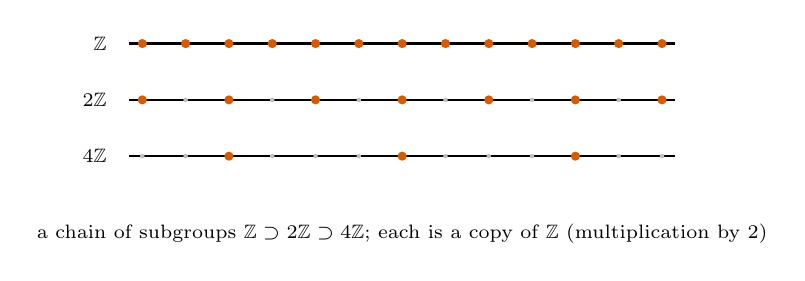
\begin{tikzpicture}[scale=0.55]
  \foreach \k/\lab/\step in {0/$\Z$/1, 1/$2\Z$/2, 2/$4\Z$/4} {
    \draw[thick] (-6.3,-1.3*\k) -- (6.3,-1.3*\k);
    \node[font=\scriptsize,anchor=east] at (-6.6,-1.3*\k) {\lab};
    \foreach \x in {-6,...,6} {\pgfmathtruncatemacro{\r}{mod(\x+12,\step)} \ifnum\r=0 \fill[mkc] (\x,-1.3*\k) circle (3pt); \else \fill[gray!50] (\x,-1.3*\k) circle (1.5pt); \fi}
  }
  \node[font=\scriptsize,align=center] at (0,-4.4) {a chain of subgroups $\Z\supset2\Z\supset4\Z$; each is a copy of $\Z$ (multiplication by $2$)};
\end{tikzpicture}}

\newcommand{\figwordpath}{%
\begin{tikzpicture}[scale=1.0,>={Stealth[length=4pt]}]
  \foreach \d/\o in {0/180,90/270,180/0,270/90} {
    \draw[gray!70] (0,0) -- (\d:2);
    \foreach \e in {0,90,180,270} {
      \ifnum\e=\o\relax\else
        \draw[gray!70] (\d:2) -- ($(\d:2)+(\e:1)$);
        \pgfmathtruncatemacro{\eo}{mod(\e+180,360)}
        \foreach \f in {0,90,180,270} {\ifnum\f=\eo\relax\else \draw[gray!50,thin] ($(\d:2)+(\e:1)$) -- ($(\d:2)+(\e:1)+(\f:0.45)$); \fi }
      \fi } }
  \fill (0,0) circle (2.5pt); \node[font=\scriptsize,below left] at (0,0) {$1$};
  \node[font=\scriptsize,below] at (2,-0.05) {$a$}; \node[font=\scriptsize,right] at (3,0) {$aa$}; \node[font=\scriptsize,right] at (2,1) {$ab$};
  % path for a a^-1 a b b^-1 a
  \draw[->,very thick,mkc] (0,0) to[bend left=35] node[above,font=\tiny] {1: $a$} (2,0);
  \draw[->,very thick,mkc] (2,0) to[bend left=35] node[below,font=\tiny] {2: $a\inv$} (0,0);
  \draw[->,very thick,mkc] (0,0) -- node[above,font=\tiny,pos=0.6] {3: $a$} (2,0);
  \draw[->,very thick,mkc] (2,0) to[bend left=35] node[left,font=\tiny] {4: $b$} (2,1);
  \draw[->,very thick,mkc] (2,1) to[bend left=35] node[right,font=\tiny] {5: $b\inv$} (2,0);
  \draw[->,very thick,mkc] (2,0) -- node[above,font=\tiny] {6: $a$} (3,0);
  \fill[mkc] (3,0) circle (3pt);
\end{tikzpicture}}

\newcommand{\figabba}{%
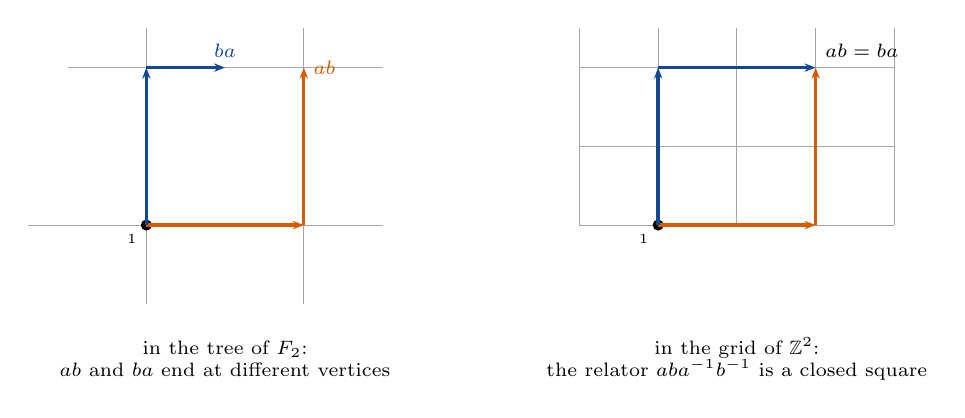
\begin{tikzpicture}[scale=1.0,>={Stealth[length=4pt]}]
  \begin{scope}
    \draw[gray!70] (-1.5,0)--(3,0); \draw[gray!70] (0,-1)--(0,2.5); \draw[gray!70] (2,-1)--(2,2.5); \draw[gray!70] (0,2)--(-1,2); \draw[gray!70] (0,2)--(1,2);
    \draw[gray!70] (2,2)--(3,2); \draw[gray!70] (2,2)--(1,2);
    \fill (0,0) circle (2pt); \node[font=\tiny,below left] at (0,0) {$1$};
    \draw[->,very thick,mkc] (0,0)--(2,0); \draw[->,very thick,mkc] (2,0)--(2,2); \node[font=\scriptsize,mkc,right] at (2,2) {$ab$};
    \draw[->,very thick,big] (0,0)--(0,2); \draw[->,very thick,big] (0,2)--(1,2); \node[font=\scriptsize,big,above] at (1,2) {$ba$};
    \node[font=\scriptsize,align=center] at (1,-1.7) {in the tree of $F_2$:\\ $ab$ and $ba$ end at different vertices};
  \end{scope}
  \begin{scope}[xshift=6.5cm]
    \draw[gray!70] (-1,0) grid (3,2.5);
    \fill (0,0) circle (2pt); \node[font=\tiny,below left] at (0,0) {$1$};
    \draw[->,very thick,mkc] (0,0)--(2,0); \draw[->,very thick,mkc] (2,0)--(2,2);
    \draw[->,very thick,big] (0,0)--(0,2); \draw[->,very thick,big] (0,2)--(2,2);
    \node[font=\scriptsize,above right] at (2,2) {$ab=ba$};
    \node[font=\scriptsize,align=center] at (1,-1.7) {in the grid of $\Z^2$:\\ the relator $aba\inv b\inv$ is a closed square};
  \end{scope}
\end{tikzpicture}}

\newcommand{\fighomdots}{%
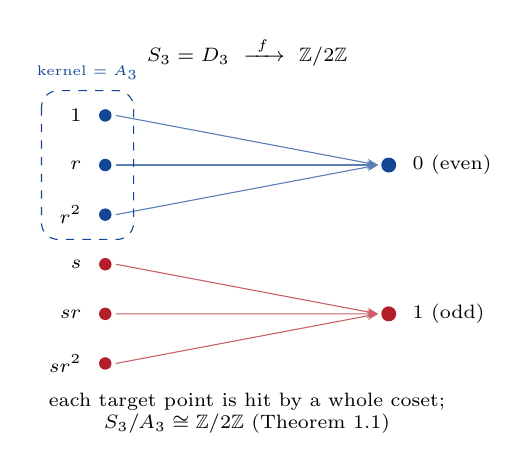
\begin{tikzpicture}[>={Stealth[length=4pt]},scale=0.9]
  \foreach \i/\l/\c in {0/1/big,1/r/big,2/r^2/big,3/s/pit,4/sr/pit,5/sr^2/pit} {
    \fill[\c] (0,-0.7*\i) circle (2.5pt); \node[font=\scriptsize,anchor=east] at (-0.2,-0.7*\i) {$\l$}; }
  \fill[big] (4,-0.7) circle (3pt); \node[font=\scriptsize,anchor=west] at (4.2,-0.7) {$0$ (even)};
  \fill[pit] (4,-2.8) circle (3pt); \node[font=\scriptsize,anchor=west] at (4.2,-2.8) {$1$ (odd)};
  \foreach \i in {0,1,2} \draw[->,big!70] (0.15,-0.7*\i) -- (3.85,-0.7);
  \foreach \i in {3,4,5} \draw[->,pit!70] (0.15,-0.7*\i) -- (3.85,-2.8);
  \draw[rounded corners=6pt,big,dashed] (-0.9,0.35) rectangle (0.4,-1.75); \node[font=\tiny,big] at (-0.25,0.6) {kernel $=A_3$};
  \node[font=\scriptsize] at (2,0.9) {$S_3=D_3\ \xrightarrow{\ f\ }\ \Z/2\Z$};
  \node[font=\scriptsize,align=center] at (2,-4.2) {each target point is hit by a whole coset;\\ $S_3/A_3\cong\Z/2\Z$ (Theorem 1.1)};
\end{tikzpicture}}

\newcommand{\figcosets}{%
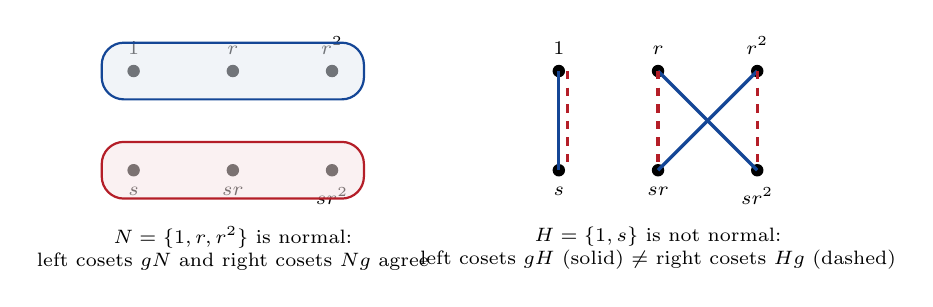
\begin{tikzpicture}[scale=0.9]
  \begin{scope}
    \foreach \j/\l in {0/1,1/r,2/r^2} {\fill (1.4*\j,0) circle (2.5pt); \node[font=\scriptsize,above] at (1.4*\j,0.1) {$\l$};}
    \foreach \j/\l in {0/s,1/sr,2/sr^2} {\fill (1.4*\j,-1.4) circle (2.5pt); \node[font=\scriptsize,below] at (1.4*\j,-1.5) {$\l$};}
    \draw[rounded corners=8pt,fill=big!12,draw=big,thick,fill opacity=0.5] (-0.45,-0.4) rectangle (3.25,0.4);
    \draw[rounded corners=8pt,fill=pit!12,draw=pit,thick,fill opacity=0.5] (-0.45,-1.8) rectangle (3.25,-1.0);
    \node[font=\scriptsize,align=center] at (1.4,-2.5) {$N=\{1,r,r^2\}$ is normal:\\ left cosets $gN$ and right cosets $Ng$ agree};
  \end{scope}
  \begin{scope}[xshift=6cm]
    \foreach \j/\l in {0/1,1/r,2/r^2} {\fill (1.4*\j,0) circle (2.5pt); \node[font=\scriptsize,above] at (1.4*\j,0.1) {$\l$};}
    \foreach \j/\l in {0/s,1/sr,2/sr^2} {\fill (1.4*\j,-1.4) circle (2.5pt); \node[font=\scriptsize,below] at (1.4*\j,-1.5) {$\l$};}
    % left cosets of H={1,s}: {1,s},{r,sr^2},{r^2,sr}  solid
    \draw[very thick,big] (0,0)--(0,-1.4);
    \draw[very thick,big] (1.4,0)--(2.8,-1.4);
    \draw[very thick,big] (2.8,0)--(1.4,-1.4);
    % right cosets: {1,s},{r,sr},{r^2,sr^2} dashed
    \draw[very thick,pit,dashed] (0.12,0)--(0.12,-1.4);
    \draw[very thick,pit,dashed] (1.4,0)--(1.4,-1.4);
    \draw[very thick,pit,dashed] (2.8,0)--(2.8,-1.4);
    \node[font=\scriptsize,align=center] at (1.4,-2.5) {$H=\{1,s\}$ is not normal:\\ left cosets $gH$ (solid) $\neq$ right cosets $Hg$ (dashed)};
  \end{scope}
\end{tikzpicture}}

\newcommand{\figcayleygallery}{%
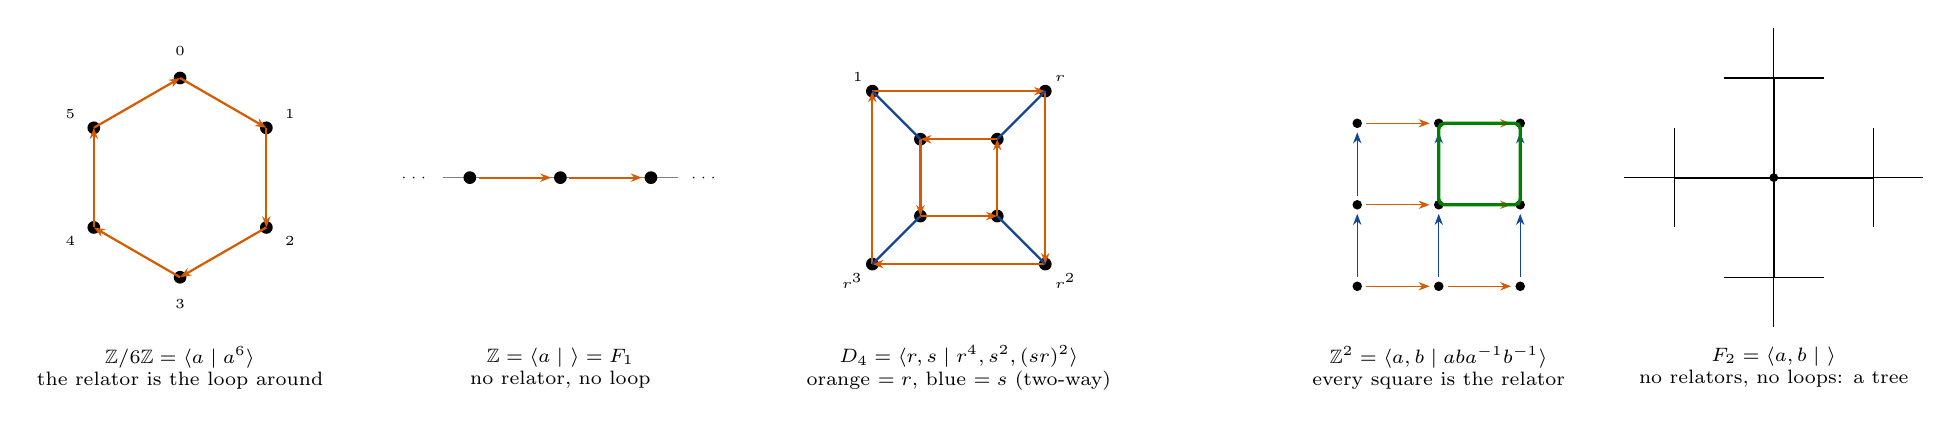
\begin{tikzpicture}[>={Stealth[length=4pt]},scale=1.15]
  % Z/6Z
  \begin{scope}
    \foreach \k in {0,...,5} {\coordinate (C\k) at ({90-60*\k}:1.1); \fill (C\k) circle (2pt); \node[font=\tiny] at ({90-60*\k}:1.4) {\k};}
    \foreach \k in {0,...,5} {\pgfmathtruncatemacro{\n}{mod(\k+1,6)} \draw[->,thick,mkc] (C\k) -- (C\n);}
    \node[font=\scriptsize,align=center] at (0,-2.1) {$\Z/6\Z=\langle a\mid a^6\rangle$\\ the relator is the loop around};
  \end{scope}
  % Z
  \begin{scope}[xshift=4.2cm]
    \draw[gray] (-1.3,0)--(1.3,0);
    \foreach \x in {-1,0,1} {\fill (\x,0) circle (2pt);}
    \foreach \x in {-1,0} \draw[->,thick,mkc] (\x+0.1,0)--(\x+0.9,0);
    \node[font=\tiny] at (-1.6,0) {$\cdots$}; \node[font=\tiny] at (1.6,0) {$\cdots$};
    \node[font=\scriptsize,align=center] at (0,-2.1) {$\Z=\langle a\mid\ \rangle=F_1$\\ no relator, no loop};
  \end{scope}
  % D4
  \begin{scope}[xshift=8.6cm]
    \foreach \k/\l in {0/1,1/r,2/r^2,3/r^3} {\coordinate (O\k) at ({135-90*\k}:1.35); \fill (O\k) circle (2pt);}
    \foreach \k/\l in {0/s,1/sr^3,2/sr^2,3/sr} {\coordinate (I\k) at ({135-90*\k}:0.6); \fill (I\k) circle (2pt);}
    \node[font=\tiny,above left] at (O0) {$1$}; \node[font=\tiny,above right] at (O1) {$r$}; \node[font=\tiny,below right] at (O2) {$r^2$}; \node[font=\tiny,below left] at (O3) {$r^3$};
    \foreach \k in {0,...,3} {\pgfmathtruncatemacro{\n}{mod(\k+1,4)} \draw[->,thick,mkc] (O\k) -- (O\n);}
    % inner: s -> sr (at I3), sr -> sr^2 (I2), sr^2 -> sr^3 (I1), sr^3 -> s (I0): reversed direction
    \foreach \k in {0,...,3} {\pgfmathtruncatemacro{\n}{mod(\k+3,4)} \draw[->,thick,mkc] (I\k) -- (I\n);}
    \foreach \k in {0,...,3} \draw[thick,big] (O\k) -- (I\k);
    \node[font=\scriptsize,align=center] at (0,-2.1) {$D_4=\langle r,s\mid r^4,s^2,(sr)^2\rangle$\\ orange $=r$, blue $=s$ (two-way)};
  \end{scope}
  % Z^2
  \begin{scope}[xshift=13cm,yshift=-1.2cm]
    \foreach \x in {0,1,2} \foreach \y in {0,1,2} \fill (\x*0.9,\y*0.9) circle (1.5pt);
    \foreach \y in {0,1,2} \foreach \x in {0,1} \draw[->,mkc] (\x*0.9+0.1,\y*0.9)--(\x*0.9+0.8,\y*0.9);
    \foreach \x in {0,1,2} \foreach \y in {0,1} \draw[->,big] (\x*0.9,\y*0.9+0.1)--(\x*0.9,\y*0.9+0.8);
    \draw[very thick,green!50!black,rounded corners=2pt] (0.9,0.9) rectangle (1.8,1.8);
    \node[font=\scriptsize,align=center] at (0.9,-0.9) {$\Z^2=\langle a,b\mid aba\inv b\inv\rangle$\\ every square is the relator};
  \end{scope}
  % F2
  \begin{scope}[xshift=17.6cm,scale=0.55]
    \foreach \d/\o in {0/180,90/270,180/0,270/90} {\draw[thick] (0,0) -- (\d:2);
      \foreach \e in {0,90,180,270} {\ifnum\e=\o\relax\else \draw (\d:2) -- ($(\d:2)+(\e:1)$); \fi}}
    \fill (0,0) circle (2.5pt);
    \node[font=\scriptsize,align=center] at (0,-3.8) {$F_2=\langle a,b\mid\ \rangle$\\ no relators, no loops: a tree};
  \end{scope}
\end{tikzpicture}}

% ===================== chapter 2 : extra figures =====================
\newcommand{\figactionhom}{%
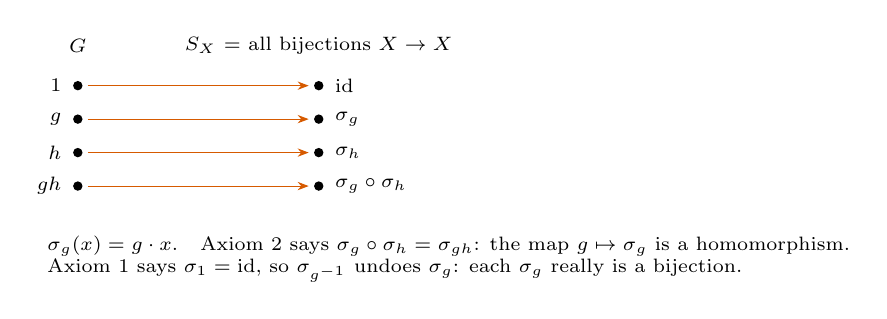
\begin{tikzpicture}[>={Stealth[length=4pt]},scale=0.85]
  \node[font=\scriptsize] at (0,1.5) {$G$};
  \foreach \i/\l in {0/1,1/g,2/h,3/gh} {\fill (0,-0.5*\i+0.9) circle (2pt); \node[font=\scriptsize,left] at (-0.1,-0.5*\i+0.9) {$\l$};}
  \node[font=\scriptsize] at (3.6,1.5) {$S_X$ = all bijections $X\to X$};
  \foreach \i/\l in {0/\mathrm{id},1/\sigma_g,2/\sigma_h,3/\sigma_g\circ\sigma_h} {\fill (3.6,-0.5*\i+0.9) circle (2pt); \node[font=\scriptsize,right] at (3.7,-0.5*\i+0.9) {$\l$};}
  \foreach \i in {0,1,2,3} \draw[->,mkc] (0.15,-0.5*\i+0.9) -- (3.45,-0.5*\i+0.9);
  \node[font=\scriptsize,align=left,anchor=north west] at (-0.6,-1.2) {$\sigma_g(x)=g\cdot x$.\quad Axiom 2 says $\sigma_g\circ\sigma_h=\sigma_{gh}$: the map $g\mapsto\sigma_g$ is a homomorphism.\\ Axiom 1 says $\sigma_1=\mathrm{id}$, so $\sigma_{g\inv}$ undoes $\sigma_g$: each $\sigma_g$ really is a bijection.};
\end{tikzpicture}}

\newcommand{\figorbits}{%
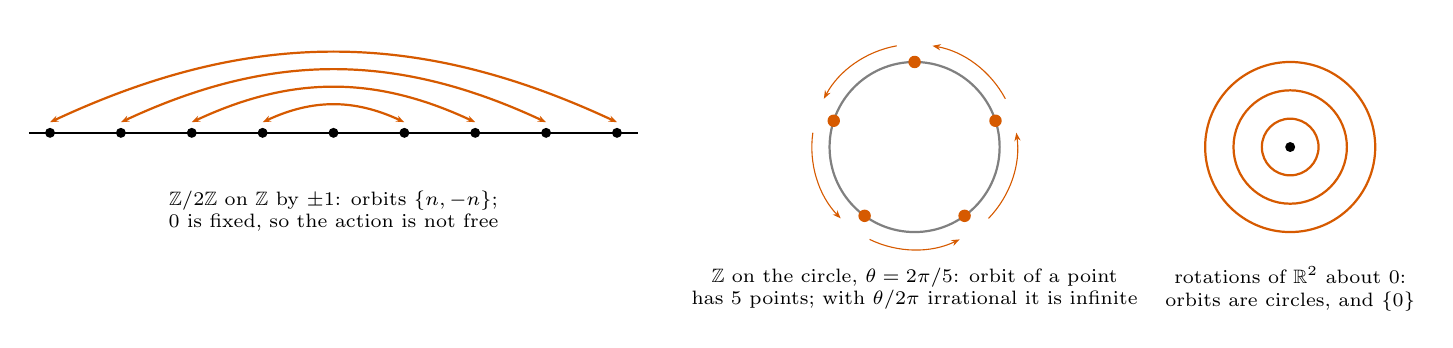
\begin{tikzpicture}[scale=0.9]
  % Z/2Z on Z
  \begin{scope}
    \draw[thick] (-4.3,0)--(4.3,0);
    \foreach \x in {-4,...,4} \fill (\x,0) circle (2pt);
    \foreach \x in {1,...,4} \draw[<->,mkc,thick,>={Stealth[length=3pt]}] (-\x,0.15) to[bend left=25] (\x,0.15);
    \node[font=\scriptsize,align=center] at (0,-1.1) {$\Z/2\Z$ on $\Z$ by $\pm1$: orbits $\{n,-n\}$;\\ $0$ is fixed, so the action is not free};
  \end{scope}
  % rotation orbit on circle
  \begin{scope}[xshift=8.2cm,yshift=-0.2cm]
    \draw[thick,gray] (0,0) circle (1.2);
    \foreach \k in {0,...,4} {\fill[mkc] ({90+72*\k}:1.2) circle (2.5pt);}
    \foreach \k in {0,...,4} {\draw[->,mkc,>={Stealth[length=3pt]}] ({90+72*\k+10}:1.45) arc ({90+72*\k+10}:{90+72*\k+62}:1.45);}
    \node[font=\scriptsize,align=center] at (0,-2.0) {$\Z$ on the circle, $\theta=2\pi/5$: orbit of a point\\ has 5 points; with $\theta/2\pi$ irrational it is infinite};
  \end{scope}
  % concentric circles: rotation orbits in the plane
  \begin{scope}[xshift=13.5cm,yshift=-0.2cm]
    \foreach \r in {0.4,0.8,1.2} \draw[mkc,thick] (0,0) circle (\r);
    \fill (0,0) circle (2pt);
    \node[font=\scriptsize,align=center] at (0,-2.0) {rotations of $\R^2$ about $0$:\\ orbits are circles, and $\{0\}$};
  \end{scope}
\end{tikzpicture}}

\newcommand{\figconjS}{%
\begin{tabular}{@{}lll@{}}
\toprule
conjugacy class in $S_3$ & elements & cycle type\\
\midrule
identity & $1$ & $1\,1\,1$\\
transpositions & $(1\,2),\ (1\,3),\ (2\,3)$ & $2\,1$\\
3-cycles & $(1\,2\,3),\ (1\,3\,2)$ & $3$\\
\bottomrule
\end{tabular}}

\newcommand{\figgraphformal}{%
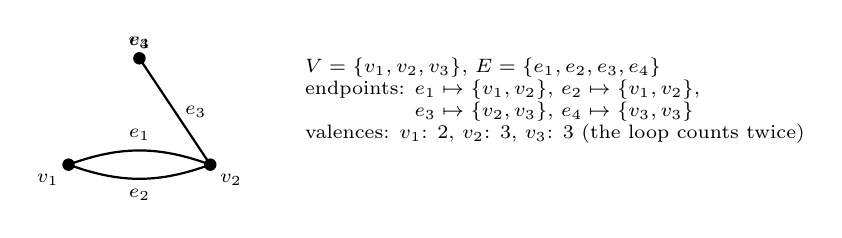
\begin{tikzpicture}[scale=0.9]
  \fill (0,0) circle (2.5pt) node[font=\scriptsize,below left] {$v_1$};
  \fill (2,0) circle (2.5pt) node[font=\scriptsize,below right] {$v_2$};
  \fill (1,1.5) circle (2.5pt) node[font=\scriptsize,above] {$v_3$};
  \draw[thick] (0,0) to[bend left=20] node[font=\scriptsize,above] {$e_1$} (2,0);
  \draw[thick] (0,0) to[bend right=20] node[font=\scriptsize,below] {$e_2$} (2,0);
  \draw[thick] (2,0) -- node[font=\scriptsize,right] {$e_3$} (1,1.5);
  \draw[thick] (1,1.5) to[out=120,in=60,looseness=8] node[font=\scriptsize,above] {$e_4$} (1,1.5);
  \node[font=\scriptsize,anchor=west,align=left] at (3.2,0.9) {$V=\{v_1,v_2,v_3\}$,\ $E=\{e_1,e_2,e_3,e_4\}$\\ endpoints: $e_1\mapsto\{v_1,v_2\}$, $e_2\mapsto\{v_1,v_2\}$,\\ \phantom{endpoints: }$e_3\mapsto\{v_2,v_3\}$, $e_4\mapsto\{v_3,v_3\}$\\ valences: $v_1$: 2,\ $v_2$: 3,\ $v_3$: 3 (the loop counts twice)};
\end{tikzpicture}}

\newcommand{\figcomplete}{%
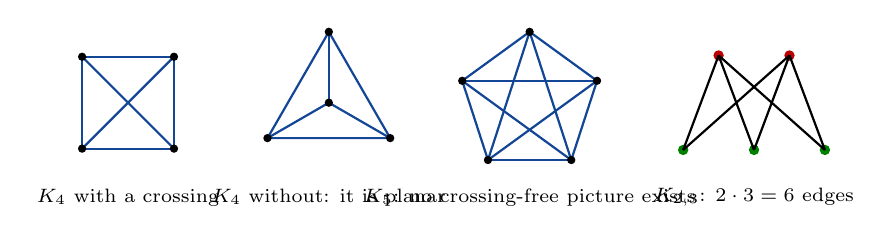
\begin{tikzpicture}[scale=0.75]
  \begin{scope}
    \foreach \k in {0,...,3} \coordinate (P\k) at ({45+90*\k}:1.1);
    \draw[thick,big] (P0)--(P1)--(P2)--(P3)--cycle; \draw[thick,big] (P0)--(P2); \draw[thick,big] (P1)--(P3);
    \foreach \k in {0,...,3} \fill (P\k) circle (2pt);
    \node[font=\scriptsize] at (0,-1.6) {$K_4$ with a crossing};
  \end{scope}
  \begin{scope}[xshift=3.4cm]
    \coordinate (A) at (90:1.2); \coordinate (B) at (210:1.2); \coordinate (C) at (330:1.2); \coordinate (D) at (0,0);
    \draw[thick,big] (A)--(B)--(C)--cycle; \draw[thick,big] (A)--(D); \draw[thick,big] (B)--(D); \draw[thick,big] (C)--(D);
    \foreach \p in {A,B,C,D} \fill (\p) circle (2pt);
    \node[font=\scriptsize] at (0,-1.6) {$K_4$ without: it is planar};
  \end{scope}
  \begin{scope}[xshift=6.8cm]
    \foreach \k in {0,...,4} \coordinate (Q\k) at ({90+72*\k}:1.2);
    \foreach \i in {0,...,4} \foreach \j in {0,...,4} {\ifnum\i<\j \draw[thick,big] (Q\i)--(Q\j); \fi}
    \foreach \k in {0,...,4} \fill (Q\k) circle (2pt);
    \node[font=\scriptsize] at (0,-1.6) {$K_5$: no crossing-free picture exists};
  \end{scope}
  \begin{scope}[xshift=10.6cm]
    \foreach \i in {0,1} \fill[red!75!black] (\i*1.2-0.6,0.8) circle (2.5pt);
    \foreach \j in {0,1,2} \fill[green!50!black] (\j*1.2-1.2,-0.8) circle (2.5pt);
    \foreach \i in {0,1} \foreach \j in {0,1,2} \draw[thick] (\i*1.2-0.6,0.8)--(\j*1.2-1.2,-0.8);
    \node[font=\scriptsize] at (0,-1.6) {$K_{2,3}$: $2\cdot3=6$ edges};
  \end{scope}
\end{tikzpicture}}

\newcommand{\figpetersen}{%
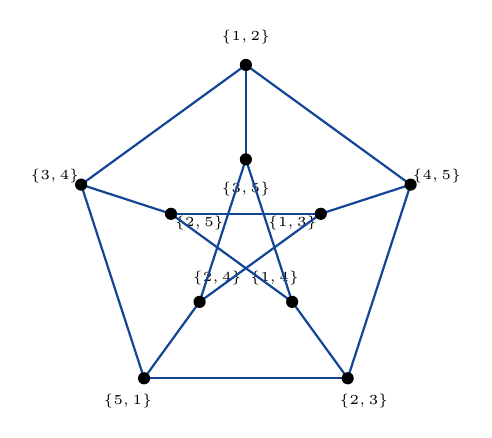
\begin{tikzpicture}[scale=1.0]
  \foreach \k/\l in {0/{1,2},1/{3,4},2/{5,1},3/{2,3},4/{4,5}} {\coordinate (O\k) at ({90+72*\k}:2.2); \node[font=\tiny,fill=white,inner sep=1pt] at ({90+72*\k}:2.55) {$\{\l\}$};}
  \foreach \k/\l in {0/{3,5},1/{2,5},2/{2,4},3/{1,4},4/{1,3}} {\coordinate (I\k) at ({90+72*\k}:1.0); \node[font=\tiny,fill=white,inner sep=1pt] at ({90+72*\k}:0.62) {$\{\l\}$};}
  \foreach \k in {0,...,4} {\pgfmathtruncatemacro{\n}{mod(\k+1,5)} \draw[thick,big] (O\k)--(O\n); \draw[thick,big] (O\k)--(I\k);}
  \foreach \k in {0,...,4} {\pgfmathtruncatemacro{\n}{mod(\k+2,5)} \draw[thick,big] (I\k)--(I\n);}
  \foreach \k in {0,...,4} {\fill (O\k) circle (2.2pt); \fill (I\k) circle (2.2pt);}
\end{tikzpicture}}

\newcommand{\figTthree}{%
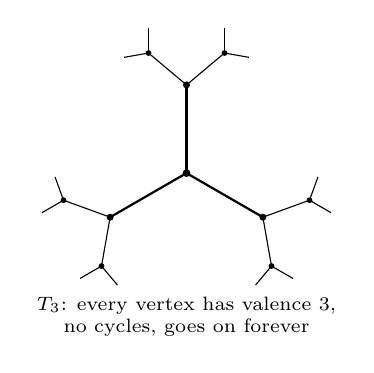
\begin{tikzpicture}[scale=0.7]
  \fill (0,0) circle (2pt);
  \foreach \d in {90,210,330} {
    \draw[thick] (0,0) -- (\d:1.6);
    \fill (\d:1.6) circle (1.8pt);
    \foreach \e in {-50,50} {
      \draw (\d:1.6) -- ($(\d:1.6)+(\d+\e:0.9)$);
      \fill ($(\d:1.6)+(\d+\e:0.9)$) circle (1.5pt);
      \foreach \f in {-50,50} {\draw[thin] ($(\d:1.6)+(\d+\e:0.9)$) -- ($(\d:1.6)+(\d+\e:0.9)+(\d+\e+\f:0.45)$);}
    }}
  \node[font=\scriptsize,align=center] at (0,-2.6) {$T_3$: every vertex has valence 3,\\ no cycles, goes on forever};
\end{tikzpicture}}

\newcommand{\figcubeiso}{%
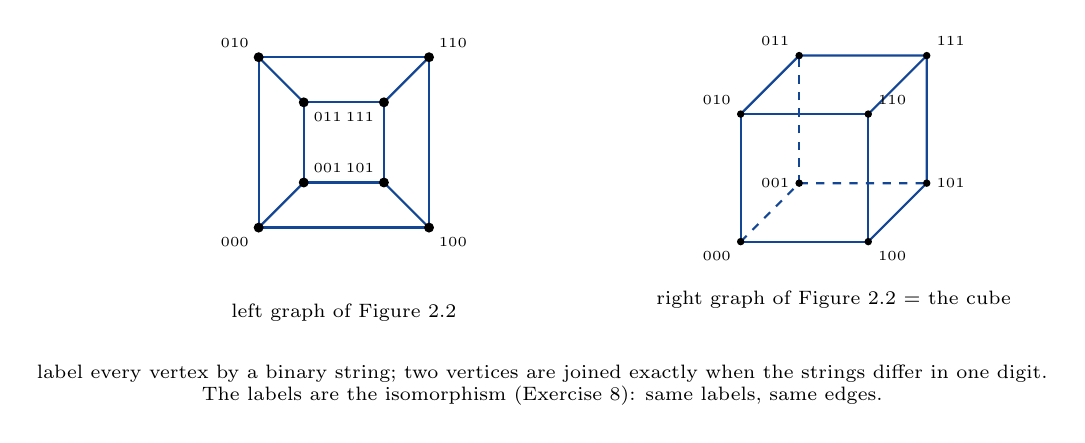
\begin{tikzpicture}[scale=0.9]
  \begin{scope}
    \foreach \k/\l in {0/010,1/110,2/100,3/000} \coordinate (O\k) at ({135-90*\k}:1.7);
    \foreach \k/\l in {0/011,1/111,2/101,3/001} \coordinate (I\k) at ({135-90*\k}:0.8);
    \foreach \k in {0,...,3} {\pgfmathtruncatemacro{\n}{mod(\k+1,4)} \draw[thick,big] (O\k)--(O\n); \draw[thick,big] (I\k)--(I\n); \draw[thick,big] (O\k)--(I\k);}
    \foreach \k/\l/\p in {0/010/above left,1/110/above right,2/100/below right,3/000/below left} {\fill (O\k) circle (2pt); \node[font=\tiny,\p] at (O\k) {\l};}
    \foreach \k/\l/\p in {0/011/below right,1/111/below left,2/101/above left,3/001/above right} {\fill (I\k) circle (2pt); \node[font=\tiny,\p] at (I\k) {\l};}
    \node[font=\scriptsize] at (0,-2.4) {left graph of Figure 2.2};
  \end{scope}
  \begin{scope}[xshift=5.6cm,yshift=-1.4cm,scale=0.75]
    \coordinate (A) at (0,0); \coordinate (B) at (2.4,0); \coordinate (C) at (2.4,2.4); \coordinate (D) at (0,2.4);
    \coordinate (E) at (1.1,1.1); \coordinate (F) at (3.5,1.1); \coordinate (G) at (3.5,3.5); \coordinate (H) at (1.1,3.5);
    \draw[thick,big] (A)--(B)--(C)--(D)--cycle; \draw[thick,big] (B)--(F)--(G)--(C); \draw[thick,big] (D)--(H)--(G); \draw[thick,big,dashed] (A)--(E)--(F); \draw[thick,big,dashed] (E)--(H);
    \foreach \p/\l/\pos in {A/000/below left,B/100/below right,C/110/above right,D/010/above left,E/001/left,F/101/right,G/111/above right,H/011/above left} {\fill (\p) circle (2pt); \node[font=\tiny,\pos] at (\p) {\l};}
    \node[font=\scriptsize] at (1.75,-1.1) {right graph of Figure 2.2 = the cube};
  \end{scope}
  \node[font=\scriptsize,align=center,anchor=north] at (2.8,-3.0) {label every vertex by a binary string; two vertices are joined exactly when the strings differ in one digit.\\ The labels are the isomorphism (Exercise 8): same labels, same edges.};
\end{tikzpicture}}

\newcommand{\figtwins}{%
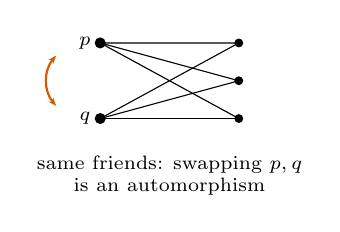
\begin{tikzpicture}[scale=0.8]
  \fill (0,0) circle (2.5pt) node[font=\scriptsize,left] {$p$};
  \fill (0,-1.2) circle (2.5pt) node[font=\scriptsize,left] {$q$};
  \foreach \i in {0,1,2} {\fill (2.2,-1.2+0.6*\i) circle (2pt); \draw (0,0)--(2.2,-1.2+0.6*\i); \draw (0,-1.2)--(2.2,-1.2+0.6*\i);}
  \draw[<->,mkc,thick,>={Stealth[length=3pt]}] (-0.7,-0.2) to[bend right=40] (-0.7,-1.0);
  \node[font=\scriptsize,align=center] at (1.1,-2.1) {same friends: swapping $p,q$\\ is an automorphism};
\end{tikzpicture}}

\newcommand{\figcayleyZtt}{%
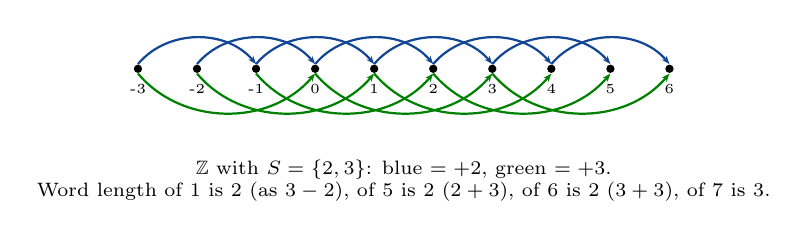
\begin{tikzpicture}[scale=0.75,>={Stealth[length=3pt]}]
  \foreach \x in {-3,...,6} {\fill (\x,0) circle (2pt); \node[font=\tiny] at (\x,-0.35) {\x};}
  \foreach \x in {-3,...,4} \draw[->,thick,big] (\x,0.08) to[bend left=50] (\x+2,0.08);
  \foreach \x in {-3,...,3} \draw[->,thick,green!50!black] (\x,-0.08) to[bend right=50] (\x+3,-0.08);
  \node[font=\scriptsize,align=center] at (1.5,-1.9) {$\Z$ with $S=\{2,3\}$: blue $=+2$, green $=+3$.\\ Word length of $1$ is $2$ (as $3-2$), of $5$ is $2$ ($2+3$), of $6$ is $2$ ($3+3$), of $7$ is $3$.};
\end{tikzpicture}}

\newcommand{\figcayleyDfour}{%
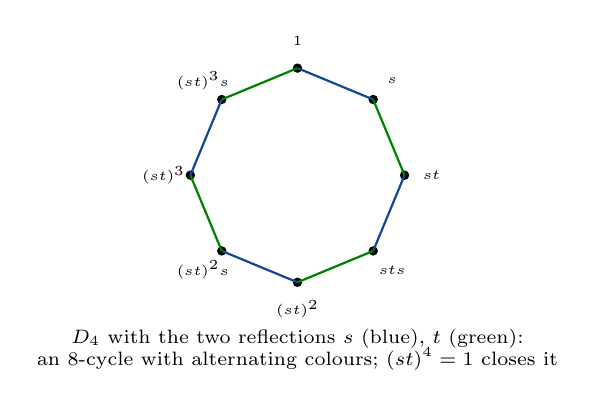
\begin{tikzpicture}[scale=0.85]
  \foreach \k/\l in {0/1,1/s,2/st,3/sts,4/(st)^2,5/(st)^2s,6/(st)^3,7/(st)^3s} {\coordinate (P\k) at ({90-45*\k}:1.6); \fill (P\k) circle (2pt); \node[font=\tiny] at ({90-45*\k}:2.0) {$\l$};}
  \foreach \k in {0,2,4,6} {\pgfmathtruncatemacro{\n}{\k+1} \draw[thick,big] (P\k)--(P\n);}
  \foreach \k in {1,3,5,7} {\pgfmathtruncatemacro{\n}{mod(\k+1,8)} \draw[thick,green!50!black] (P\k)--(P\n);}
  \node[font=\scriptsize,align=center] at (0,-2.6) {$D_4$ with the two reflections $s$ (blue), $t$ (green):\\ an 8-cycle with alternating colours; $(st)^4=1$ closes it};
\end{tikzpicture}}

\newcommand{\figcayleySthree}{%
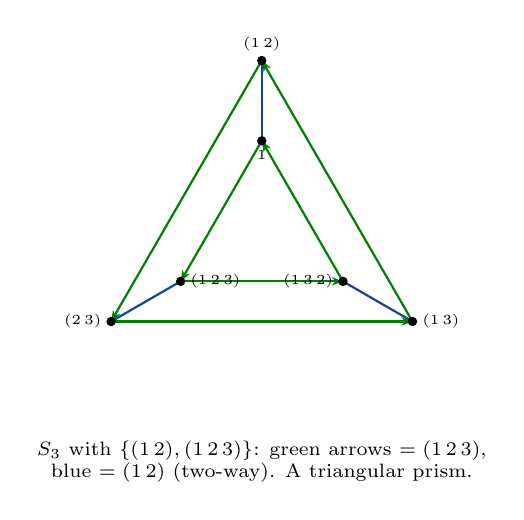
\begin{tikzpicture}[scale=0.85,>={Stealth[length=4pt]}]
  \coordinate (A) at (90:1.4); \coordinate (B) at (210:1.4); \coordinate (C) at (330:1.4);
  \coordinate (D) at (90:2.6); \coordinate (E) at (210:2.6); \coordinate (F) at (330:2.6);
  \draw[->,thick,green!50!black] (A)--(B); \draw[->,thick,green!50!black] (B)--(C); \draw[->,thick,green!50!black] (C)--(A);
  \draw[->,thick,green!50!black] (D)--(E); \draw[->,thick,green!50!black] (E)--(F); \draw[->,thick,green!50!black] (F)--(D);
  \draw[thick,big] (A)--(D); \draw[thick,big] (B)--(E); \draw[thick,big] (C)--(F);
  \foreach \p/\l/\pos in {A/1/below,B/(1\,2\,3)/right,C/(1\,3\,2)/left,D/(1\,2)/above,E/(2\,3)/left,F/(1\,3)/right} {\fill (\p) circle (2pt); \node[font=\tiny,\pos] at (\p) {$\l$};}
  \node[font=\scriptsize,align=center] at (0,-3.4) {$S_3$ with $\{(1\,2),(1\,2\,3)\}$: green arrows $=(1\,2\,3)$,\\ blue $=(1\,2)$ (two-way). A triangular prism.};
\end{tikzpicture}}

\newcommand{\figballs}{%
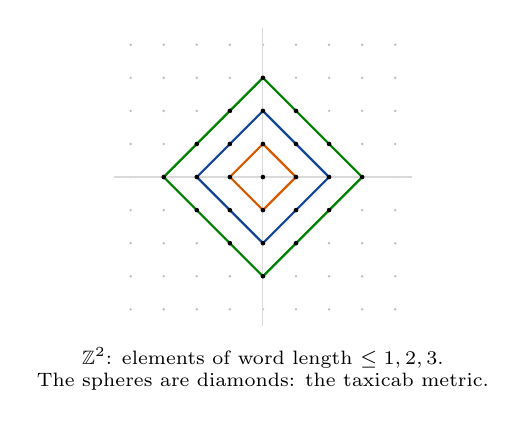
\begin{tikzpicture}[scale=0.42]
  \foreach \x in {-4,...,4} \foreach \y in {-4,...,4} \fill[gray!50] (\x,\y) circle (1.2pt);
  \draw[gray!30] (-4.5,0)--(4.5,0); \draw[gray!30] (0,-4.5)--(0,4.5);
  \foreach \r/\c in {1/mkc,2/big,3/green!50!black} {\draw[thick,\c] (\r,0)--(0,\r)--(-\r,0)--(0,-\r)--cycle;}
  \foreach \x in {-3,...,3} \foreach \y in {-3,...,3} {\pgfmathtruncatemacro{\d}{abs(\x)+abs(\y)} \ifnum\d<4 \fill (\x,\y) circle (2pt); \fi}
  \node[font=\scriptsize,align=center] at (0,-5.8) {$\Z^2$: elements of word length $\le1,2,3$.\\ The spheres are diamonds: the taxicab metric.};
\end{tikzpicture}}

\newcommand{\figtranslate}{%
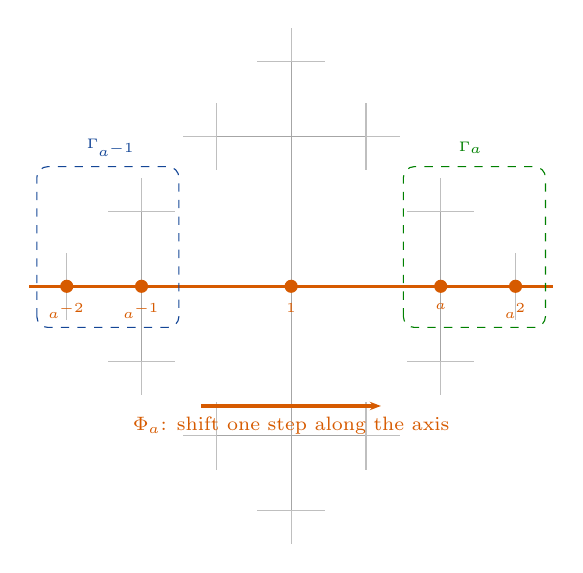
\begin{tikzpicture}[scale=0.95,>={Stealth[length=4pt]}]
  \foreach \d/\o in {0/180,90/270,180/0,270/90} {
    \draw[gray!70] (0,0) -- (\d:2);
    \foreach \e in {0,90,180,270} {\ifnum\e=\o\relax\else \draw[gray!70] (\d:2) -- ($(\d:2)+(\e:1)$);
      \pgfmathtruncatemacro{\eo}{mod(\e+180,360)}
      \foreach \f in {0,90,180,270} {\ifnum\f=\eo\relax\else \draw[gray!50,thin] ($(\d:2)+(\e:1)$) -- ($(\d:2)+(\e:1)+(\f:0.45)$); \fi } \fi } }
  \draw[very thick,mkc] (-3.5,0)--(3.5,0);
  \foreach \x/\l in {-3/a^{-2},-2/a\inv,0/1,2/a,3/a^2} {\fill[mkc] (\x,0) circle (2.5pt); \node[font=\tiny,below,mkc] at (\x,-0.1) {$\l$};}
  \draw[->,very thick,mkc] (-1.2,-1.6) -- node[below,font=\scriptsize] {$\Phi_a$: shift one step along the axis} (1.2,-1.6);
  \draw[rounded corners=4pt,big,dashed] (-3.4,-0.55) rectangle (-1.5,1.6); \node[font=\tiny,big] at (-2.4,1.85) {$\Gamma_{a\inv}$};
  \draw[rounded corners=4pt,green!50!black,dashed] (1.5,-0.55) rectangle (3.4,1.6); \node[font=\tiny,green!50!black] at (2.4,1.85) {$\Gamma_a$};
\end{tikzpicture}}

\newcommand{\figproofpic}{%
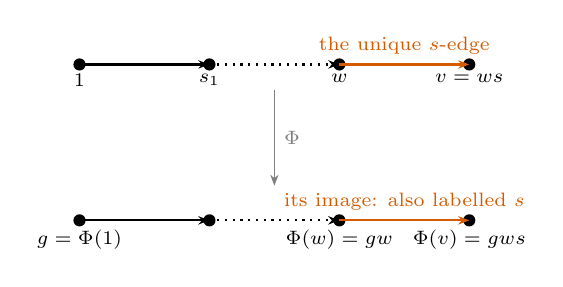
\begin{tikzpicture}[>={Stealth[length=4pt]},scale=1.1]
  \fill (0,0) circle (2pt) node[font=\scriptsize,below] {$1$};
  \fill (1.5,0) circle (2pt) node[font=\scriptsize,below] {$s_1$};
  \fill (3,0) circle (2pt) node[font=\scriptsize,below] {$w$};
  \fill (4.5,0) circle (2pt) node[font=\scriptsize,below] {$v=ws$};
  \draw[->,thick] (0,0)--(1.5,0); \draw[->,thick,dotted] (1.5,0)--(3,0); \draw[->,thick,mkc] (3,0)-- node[above,font=\scriptsize] {the unique $s$-edge} (4.5,0);
  \fill (0,-1.8) circle (2pt) node[font=\scriptsize,below] {$g=\Phi(1)$};
  \fill (1.5,-1.8) circle (2pt); \fill (3,-1.8) circle (2pt) node[font=\scriptsize,below] {$\Phi(w)=gw$};
  \fill (4.5,-1.8) circle (2pt) node[font=\scriptsize,below] {$\Phi(v)=gws$};
  \draw[->,thick] (0,-1.8)--(1.5,-1.8); \draw[->,thick,dotted] (1.5,-1.8)--(3,-1.8); \draw[->,thick,mkc] (3,-1.8)-- node[above,font=\scriptsize] {its image: also labelled $s$} (4.5,-1.8);
  \draw[->,gray] (2.25,-0.3)-- node[right,font=\scriptsize] {$\Phi$} (2.25,-1.4);
\end{tikzpicture}}

\newcommand{\fighexsym}{%
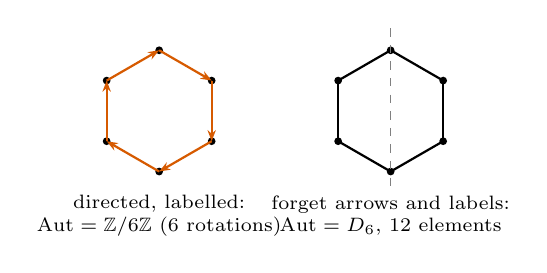
\begin{tikzpicture}[scale=0.7,>={Stealth[length=4pt]}]
  \begin{scope}
    \foreach \k in {0,...,5} {\coordinate (C\k) at ({90-60*\k}:1.1); \fill (C\k) circle (2pt);}
    \foreach \k in {0,...,5} {\pgfmathtruncatemacro{\n}{mod(\k+1,6)} \draw[->,thick,mkc] (C\k) -- (C\n);}
    \node[font=\scriptsize,align=center] at (0,-1.9) {directed, labelled:\\ $\mathrm{Aut}=\Z/6\Z$ (6 rotations)};
  \end{scope}
  \begin{scope}[xshift=4.2cm]
    \foreach \k in {0,...,5} {\coordinate (D\k) at ({90-60*\k}:1.1); \fill (D\k) circle (2pt);}
    \foreach \k in {0,...,5} {\pgfmathtruncatemacro{\n}{mod(\k+1,6)} \draw[thick] (D\k) -- (D\n);}
    \draw[dashed,gray] (0,1.5)--(0,-1.5);
    \node[font=\scriptsize,align=center] at (0,-1.9) {forget arrows and labels:\\ $\mathrm{Aut}=D_6$, 12 elements};
  \end{scope}
\end{tikzpicture}}

\newcommand{\figspheres}{%
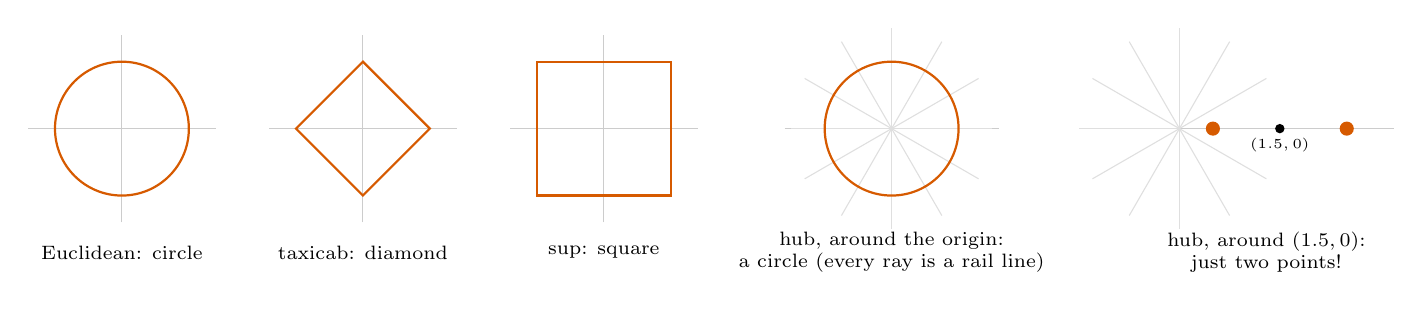
\begin{tikzpicture}[scale=0.85]
  \foreach \dx/\cap in {0/{Euclidean: circle},3.6/{taxicab: diamond},7.2/{sup: square}} {
    \begin{scope}[xshift=\dx cm]
      \draw[gray!40] (-1.4,0)--(1.4,0); \draw[gray!40] (0,-1.4)--(0,1.4);
      \node[font=\scriptsize] at (0,-1.85) {\cap};
    \end{scope}}
  \draw[thick,mkc] (0,0) circle (1);
  \draw[thick,mkc] (3.6+1,0)--(3.6,1)--(3.6-1,0)--(3.6,-1)--cycle;
  \draw[thick,mkc] (7.2-1,-1) rectangle (7.2+1,1);
  \begin{scope}[xshift=11.5cm]
    \draw[gray!40] (-1.6,0)--(1.6,0); \draw[gray!40] (0,-1.4)--(0,1.4);
    \foreach \a in {0,30,...,330} \draw[gray!25] (0,0)--(\a:1.5);
    \draw[thick,mkc] (0,0) circle (1);
    \node[font=\scriptsize,align=center] at (0,-1.85) {hub, around the origin:\\ a circle (every ray is a rail line)};
  \end{scope}
  \begin{scope}[xshift=15.8cm]
    \draw[gray!40] (-0.4,0)--(3.2,0); \draw[gray!40] (0,-1.4)--(0,1.4);
    \foreach \a in {30,60,...,330} \draw[gray!25] (0,0)--(\a:1.5);
    \fill (1.5,0) circle (2pt); \node[font=\tiny,below] at (1.5,0) {$(1.5,0)$};
    \fill[mkc] (0.5,0) circle (3pt); \fill[mkc] (2.5,0) circle (3pt);
    \node[font=\scriptsize,align=center] at (1.3,-1.85) {hub, around $(1.5,0)$:\\ just two points!};
  \end{scope}
\end{tikzpicture}}

\newcommand{\figtaxipaths}{%
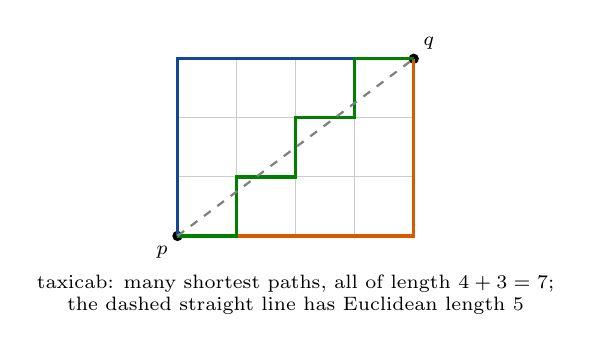
\begin{tikzpicture}[scale=0.75]
  \draw[gray!40] (0,0) grid (4,3);
  \fill (0,0) circle (2.5pt) node[font=\scriptsize,below left] {$p$}; \fill (4,3) circle (2.5pt) node[font=\scriptsize,above right] {$q$};
  \draw[very thick,mkc] (0,0)--(4,0)--(4,3);
  \draw[very thick,big] (0,0)--(0,3)--(4,3);
  \draw[very thick,green!50!black] (0,0)--(1,0)--(1,1)--(2,1)--(2,2)--(3,2)--(3,3)--(4,3);
  \draw[thick,dashed,gray] (0,0)--(4,3);
  \node[font=\scriptsize,align=center] at (2,-1.0) {taxicab: many shortest paths, all of length $4+3=7$;\\ the dashed straight line has Euclidean length $5$};
\end{tikzpicture}}

\newcommand{\fighub}{%
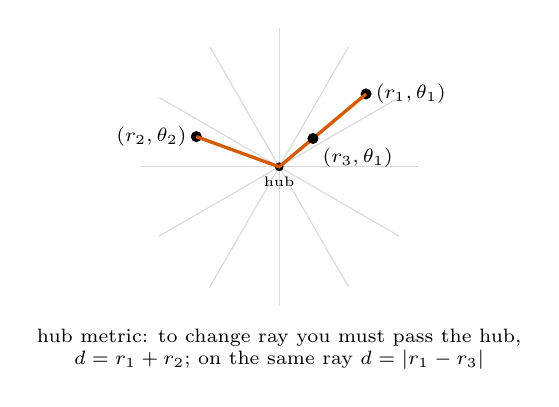
\begin{tikzpicture}[scale=0.8]
  \foreach \a in {0,30,...,330} \draw[gray!30] (0,0)--(\a:2.2);
  \fill (0,0) circle (2pt) node[font=\tiny,below] {hub};
  \fill (40:1.8) circle (2.5pt) node[font=\scriptsize,right] {$(r_1,\theta_1)$};
  \fill (160:1.4) circle (2.5pt) node[font=\scriptsize,left] {$(r_2,\theta_2)$};
  \draw[very thick,mkc] (40:1.8)--(0,0)--(160:1.4);
  \fill (40:0.7) circle (2.5pt) node[font=\scriptsize,below right] {$(r_3,\theta_1)$};
  \node[font=\scriptsize,align=center] at (0,-2.9) {hub metric: to change ray you must pass the hub,\\ $d=r_1+r_2$; on the same ray $d=|r_1-r_3|$};
\end{tikzpicture}}

\newcommand{\figLone}{%
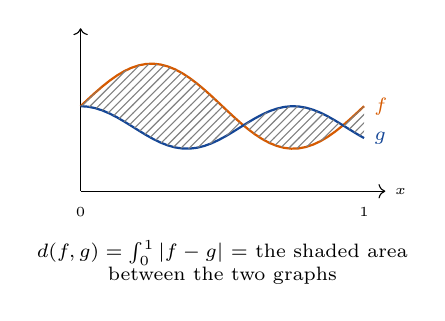
\begin{tikzpicture}[scale=0.9]
  \draw[->] (0,0)--(4.3,0) node[right,font=\tiny] {$x$}; \draw[->] (0,0)--(0,2.3);
  \draw[thick,mkc,domain=0:4,samples=40] plot (\x,{1.2+0.6*sin(\x*90)}) node[right,font=\scriptsize] {$f$};
  \draw[thick,big,domain=0:4,samples=40] plot (\x,{0.9+0.3*cos(\x*120)}) node[right,font=\scriptsize] {$g$};
  \fill[pattern=north east lines,pattern color=gray] plot[domain=0:4,samples=40] (\x,{1.2+0.6*sin(\x*90)}) -- plot[domain=4:0,samples=40] (\x,{0.9+0.3*cos(\x*120)}) -- cycle;
  \node[font=\tiny] at (0,-0.3) {$0$}; \node[font=\tiny] at (4,-0.3) {$1$};
  \node[font=\scriptsize,align=center] at (2,-1.0) {$d(f,g)=\int_0^1|f-g|$ = the shaded area\\ between the two graphs};
\end{tikzpicture}}

\newcommand{\figrealization}{%
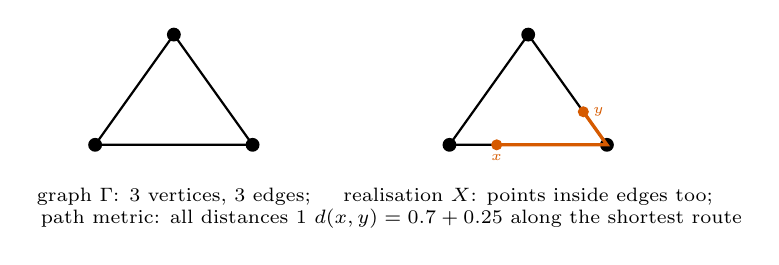
\begin{tikzpicture}[scale=1.0]
  \begin{scope}
    \fill (0,0) circle (2.5pt); \fill (2,0) circle (2.5pt); \fill (1,1.4) circle (2.5pt);
    \draw[thick] (0,0)--(2,0)--(1,1.4)--cycle;
    \node[font=\scriptsize,align=center] at (1,-0.8) {graph $\Gamma$: 3 vertices, 3 edges;\\ path metric: all distances $1$};
  \end{scope}
  \begin{scope}[xshift=4.5cm]
    \fill (0,0) circle (2.5pt); \fill (2,0) circle (2.5pt); \fill (1,1.4) circle (2.5pt);
    \draw[thick] (0,0)--(2,0)--(1,1.4)--cycle;
    \fill[mkc] (0.6,0) circle (2pt) node[below,font=\tiny] {$x$}; \fill[mkc] (1.7,0.42) circle (2pt) node[right,font=\tiny] {$y$};
    \draw[very thick,mkc] (0.6,0)--(2,0)--(1.7,0.42);
    \node[font=\scriptsize,align=center] at (1,-0.8) {realisation $X$: points inside edges too;\\ $d(x,y)=0.7+0.25$ along the shortest route};
  \end{scope}
\end{tikzpicture}}

\newcommand{\figcentroid}{%
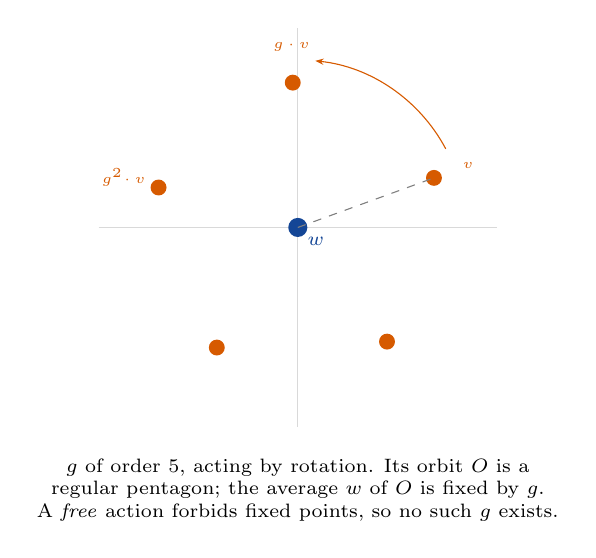
\begin{tikzpicture}[scale=1.15]
  \draw[gray!30] (-2.2,0)--(2.2,0); \draw[gray!30] (0,-2.2)--(0,2.2);
  \foreach \k in {0,...,4} {\fill[mkc] ({20+72*\k}:1.6) circle (2.5pt);}
  \node[font=\tiny,mkc] at ({20}:2.0) {$v$}; \node[font=\tiny,mkc] at ({92}:2.0) {$g\cdot v$}; \node[font=\tiny,mkc] at ({164}:2.0) {$g^2\!\cdot v$};
  \draw[->,>={Stealth[length=3pt]},mkc] ({20+8}:1.85) arc ({28}:{84}:1.85);
  \fill[big] (0,0) circle (3pt); \node[font=\scriptsize,big,below right] at (0,0) {$w$};
  \draw[dashed,gray] (0,0) -- ({20}:1.6);
  \node[font=\scriptsize,align=center] at (0,-2.9) {$g$ of order 5, acting by rotation. Its orbit $O$ is a\\ regular pentagon; the average $w$ of $O$ is fixed by $g$.\\ A \emph{free} action forbids fixed points, so no such $g$ exists.};
\end{tikzpicture}}

\newcommand{\figsimplex}{%
\begin{tikzpicture}[scale=0.8]
  \fill (0,0) circle (2pt); \fill (1.5,0) circle (2pt); \draw[thick] (0,0)--(1.5,0);
  \node[font=\tiny] at (0.75,-0.6) {1-simplex};
  \begin{scope}[xshift=3cm]
    \draw[thick] (0,0)--(1.5,0)--(0.75,1.3)--cycle; \foreach \p in {(0,0),(1.5,0),(0.75,1.3)} \fill \p circle (2pt);
    \node[font=\tiny] at (0.75,-0.6) {2-simplex};
  \end{scope}
  \begin{scope}[xshift=6cm]
    \draw[thick] (0,0)--(1.6,0)--(1.1,1.4)--cycle; \draw[thick] (0,0)--(0.6,0.5)--(1.6,0); \draw[thick,dashed] (0.6,0.5)--(1.1,1.4);
    \foreach \p in {(0,0),(1.6,0),(1.1,1.4),(0.6,0.5)} \fill \p circle (2pt);
    \node[font=\tiny] at (0.8,-0.6) {3-simplex};
  \end{scope}
\end{tikzpicture}}

\newcommand{\figwordmetricD}{%
\begin{tabular}{@{}c|cccccc@{}}
$d$ & $1$ & $s$ & $t$ & $st$ & $ts$ & $sts$\\ \hline
$1$ & 0 & 1 & 1 & 2 & 2 & 3\\
$s$ & 1 & 0 & 2 & 1 & 3 & 2\\
$t$ & 1 & 2 & 0 & 3 & 1 & 2\\
$st$ & 2 & 1 & 3 & 0 & 2 & 1\\
$ts$ & 2 & 3 & 1 & 2 & 0 & 1\\
$sts$ & 3 & 2 & 2 & 1 & 1 & 0\\
\end{tabular}}

\newcommand{\figmaptwo}{%
\begin{tikzpicture}[>={Stealth[length=5pt]},node distance=5mm and 7mm,
  box/.style={draw,rounded corners=3pt,align=center,font=\scriptsize,inner sep=3pt,fill=white},
  key/.style={box,fill=big!8,draw=big,thick}]
  \node[key] (act) {group action\\$G\times X\to X$ = hom $G\to S_X$};
  \node[box,right=of act] (orb) {orbits, transitive, free};
  \node[box,right=of orb] (cay) {Cayley's theorem\\$G\hookrightarrow S_G$};
  \node[key,below=of act] (graph) {graphs, isomorphisms,\\$\mathrm{Aut}(\Gamma)$};
  \node[key,right=of graph] (cg) {Cayley graph $\Gamma(G,S)$\\ paths $\leftrightarrow$ words};
  \node[key,right=of cg] (t22) {Theorem 2.2\\$G\cong\mathrm{Aut}(\Gamma(G,S))$};
  \node[key,below=of graph] (ms) {metric spaces,\\isometries, $\mathrm{Isom}(X)$};
  \node[key,right=of ms] (wm) {word metric:\\a group \emph{is} a metric space};
  \node[key,right=of wm] (t23) {Theorem 2.3\\free on $\R^n$ $\Rightarrow$ torsion free};
  \node[box,fill=ahead!8,draw=ahead,below=of wm] (q) {the big question: which groups act on which spaces,\\ and what does a group look like as a space?};
  \draw[->] (act)--(orb); \draw[->] (orb)--(cay); \draw[->] (act)--(graph); \draw[->] (graph)--(cg); \draw[->] (cg)--(t22);
  \draw[->] (graph)--(ms); \draw[->] (cg)--(wm); \draw[->] (ms)--(wm); \draw[->] (ms)--(t23); \draw[->] (wm)--(q); \draw[->] (t23)--(q);
\end{tikzpicture}}

% =====================================================================
\begin{document}

% ---------------------------------------------------------------- COVER
\begin{textblock*}{744pt}(24pt,24pt)
{\sffamily\bfseries\huge Office Hour Two: \ldots and Spaces}\par\vspace{4pt}
{\sffamily\Large An annotated study edition}\par\vspace{6pt}
{\large Original chapter: Matt Clay and Dan Margalit, \emph{Office Hours with a Geometric Group Theorist} (Princeton University Press, 2017), pages 21--41.}\par
\vspace{12pt}
\begin{minipage}[t]{385pt}
{\sffamily\bfseries\large How to read this}\par\vspace{4pt}
Each spread shows one original page on the left, untouched, and a column of annotations on the right.
Orange numbered markers \num{1}\,\num{2}\,\num{3} on the page point to the line the annotation is about; a faint yellow bar marks the exact statement when it matters.
Seven full-width visual pages (V1--V7) sit between the spreads and draw the constructions that the column is too narrow for.
The level is the same as the chapter 1 edition: a strong high-school reader who has worked through Office Hour 1.

\vspace{6pt}
{\sffamily\bfseries\large Colour code for the boxes}\par\vspace{2pt}
\begin{tabular}{@{}ll@{}}
\textcolor{big}{\rule{8pt}{8pt}} Big picture & where an idea sits in the whole book\\
\textcolor{why}{\rule{8pt}{8pt}} Why? & the reason a definition or claim is true\\
\textcolor{pit}{\rule{8pt}{8pt}} Watch out & a common misreading, or a slip in the printed text\\
\textcolor{try}{\rule{8pt}{8pt}} Try it & something to check by hand, and hints for exercises\\
\textcolor{ahead}{\rule{8pt}{8pt}} Looking ahead & connections to later office hours\\
\textcolor{gray!60!black}{\rule{8pt}{8pt}} Background & facts from school mathematics the text assumes\\
\end{tabular}

\vspace{8pt}
{\sffamily\bfseries\large Contents of the chapter}\par\vspace{2pt}
\begin{tabular}{@{}lll@{}}
Group actions, orbits, Cayley's theorem & book pp.\ 21--23 & V1\\
2.1 Graphs, isomorphisms, automorphisms & book pp.\ 23--28 & V2, V3\\
Cayley graphs and Theorem 2.2 & book pp.\ 29--33 & V4, V5\\
2.2 Metric spaces, word metric, isometries & book pp.\ 34--39 & V6\\
Theorem 2.3 and 2.3 the big question & book pp.\ 40--41 & V7\\
Exercise hints (all 26) and glossary & --- & closing page\\
\end{tabular}
\end{minipage}\hfill
\begin{minipage}[t]{330pt}
\begin{bigpic}
\textbf{The one sentence to keep in mind.} Office Hour 1 said every group \emph{should} be the symmetries of something; this office hour makes it true twice.
First for graphs: $G$ is exactly the symmetry group of its Cayley graph (Theorem 2.2).
Then it turns the tables: with the word metric, $G$ \emph{is itself} a geometric object, and geometry can be used to prove algebra (Theorem 2.3).
\end{bigpic}
\begin{prereq}
Assumed from Office Hour 1: group, subgroup, homomorphism, kernel, generating set, $S_n$, $D_n$, $\Z^n$, $F_2$, reduced words.
New school-level tools used here: absolute value and the triangle inequality $|a+b|\le|a|+|b|$, Pythagoras, polar coordinates $(r,\theta)$, the notion of a bijection between infinite sets.
\end{prereq}
\vspace{4pt}
\centering\figcayleySthree\par
{\scriptsize A taste of what is coming: the Cayley graph of $S_3$ for the generators $(1\,2)$ and $(1\,2\,3)$. Every group has such a picture, and the group is precisely its set of symmetries.}
\end{minipage}
\end{textblock*}
\mbox{}\clearpage

% ================================================================ BOOK p.21
\bookpage{036}{21}{
  \mk{1}{40}{411} \hl{55}{413}{330}{12} \mk{2}{40}{459} \mk{3}{40}{538}
}
\anncol{
\A{1}{The three moves of this office hour}
(1) Make ``$G$ is a group of symmetries of $X$'' precise: a \emph{group action}. (2) Build, for any $G$, a graph whose symmetries are exactly $G$: the \emph{Cayley graph}. (3) Introduce \emph{metric spaces}, show that $G$ itself is one, and state the questions that drive the whole book.
\begin{bigpic}
Office Hour 1 went from groups to pictures example by example. Here the direction is reversed and made general: a single construction, valid for every group, produces the picture. That is why this chapter is more abstract than the first; the payoff is that from now on every group has a shape.
\end{bigpic}

\A{2}{``Groups themselves are metric spaces''}
The most important sentence on the page. A metric space is a set in which distances are defined (page 34). On page 37 the distance between two group elements $g,h$ will be the length of the shortest word taking you from $g$ to $h$. Everything from Office Hour 7 onwards depends on this idea.

\A{3}{``Does something to''}
The examples are the ones you already know: a reflection in $D_n$ moves the vertices of the polygon; a permutation in $S_n$ moves the numbers $1,\dots,n$; an integer $n\in\Z$ slides the real line by $n$. In each case a group element is a \emph{rule} that sends every point of the object to another point. ``Acts on'' is the word for this.
\begin{prereq}
A function of two variables $G\times X\to X$ takes a group element and a point and returns a point. Writing the output as $g\cdot x$ is just notation: it is not a product inside $G$ (unless $X$ happens to be $G$, as on page 23).
\end{prereq}
\begin{tryit}
Before turning the page, write the two rules you would expect a ``sensible'' action to obey. (Hint: what should the identity do, and what should ``do $h$, then do $g$'' equal?) Compare with the definition at the top of page 22.
\end{tryit}
}

% ================================================================ BOOK p.22
\bookpage{037}{22}{
  \mk{1}{52}{88} \hl{76}{116}{300}{28} \mk{2}{52}{182} \mk{3}{52}{265} \hl{67}{257}{330}{22} \mk{4}{52}{362} \mk{5}{52}{490} \mk{6}{52}{561}
}
\anncol{
\A{1}{The two axioms}
Axiom 1: the identity does nothing. Axiom 2: acting by $h$ and then by $g$ is the same as acting by the product $gh$. Note the order: $g\cdot(h\cdot x)$ applies $h$ first, and $gh$ is ``$h$ then $g$'' in the convention of Office Hour 1, page 6. So axiom 2 says the action \emph{respects the multiplication}.
\begin{pitfall}
Had we written $(hg)\cdot x$ in axiom 2 we would get a \emph{right} action, a different notion. Right multiplication $g\cdot h=hg$ is \emph{not} an action in the book's sense (check: $g\cdot(h\cdot x)=xhg$ but $(gh)\cdot x=xgh$). The fix $g\cdot h=hg\inv$ works; try it.
\end{pitfall}

\A{2}{The trivial action}
Every element does nothing. It satisfies both axioms, which shows the axioms alone do not force anything interesting to happen; page 39 returns to this with the notion of the kernel of an action.

\A{3}{An action is a homomorphism $G\to S_X$}
\begin{center}\figactionhom\end{center}
This is Exercise 1. The converse: given a homomorphism $\rho:G\to S_X$, set $g\cdot x=\rho(g)(x)$ and the axioms are exactly ``$\rho(1)=\mathrm{id}$'' and ``$\rho(gh)=\rho(g)\rho(h)$''. So the two descriptions are interchangeable, and one can pass freely between ``$G$ acts on $X$'' and ``$G$ maps to the symmetries of $X$''.

\A{4}{The six examples}
(4) $\pm1$ flips the sign. (5) $m\cdot v=A^mv$ needs $A$ invertible, since $m$ can be negative. (6) $e^{im\theta}z$ rotates $z$ by the angle $m\theta$; if $\theta/2\pi$ is irrational no point ever returns, and the orbit of $z$ is infinite and spread densely around the circle. Visual page V1 draws these.

\A{5}{Orbits, transitive, free}
The orbit of $x$ is everywhere $x$ can be sent. \emph{Transitive}: one orbit, everything reachable from everything. \emph{Free}: no element except $1$ has any fixed point.
\begin{pitfall}
``Free'' is a strong condition. $D_n$ on the vertices of the $n$-gon is transitive but not free: a reflection whose axis passes through a vertex fixes that vertex. $\Z/2\Z$ on $\Z$ by $\pm1$ is not free because $0$ is fixed. $\Z$ on the circle by an irrational rotation \emph{is} free.
\end{pitfall}

\A{6}{Exercise 3: hint}
For each example list the orbits: $S_n$ on $\{1,\dots,n\}$: one orbit. $\Z/2\Z$ on $\Z$: $\{0\}$ and the pairs $\{n,-n\}$. Rotations of the plane: circles centred at the origin, and the origin.
}

% ================================================================ INTERLUDE A (page 22: the action axioms)
\interlude{A. Page 22: the two axioms of an action, and how to test a candidate rule}{
\begin{minipage}[t]{744pt}\vspace{0pt}
\small
An action has three pieces of data: a group $G$, a set $X$, and a rule that takes a group element and a point of $X$ and returns a point of $X$. The two axioms are promises about that rule. Pictures use the convention of Office Hour 1: grey numbers are fixed \emph{positions}, and a coloured disc names the corner \emph{originally} at that position, so a disc away from its grey number has moved. Here $G=D_4$ and $X$ is the set of four corners of a square.\par\vspace{4pt}
\begin{minipage}[t]{424pt}\vspace{0pt}
{\sffamily\bfseries\color{big} Axiom 1: the identity does nothing}\par\vspace{2pt}
$1\cdot x=x$ for every $x$. This is not automatic: a rule can easily send everything to one fixed point, and such a rule is not an action.\par\nobreak\vspace{2pt}
\centerline{\begin{tikzpicture}[scale=0.85]
  \draw[thick,big] (-0.707,0.707)--(0.707,0.707)--(0.707,-0.707)--(-0.707,-0.707)--cycle;
  \node[font=\tiny,gray] at (-0.948,0.948) {1};
  \node[font=\scriptsize\bfseries,circle,inner sep=0.4pt,minimum size=11pt,fill=red!80!black!30,draw=red!80!black,thick,text=black] at (-0.707,0.707) {1};
  \node[font=\tiny,gray] at (0.948,0.948) {2};
  \node[font=\scriptsize\bfseries,circle,inner sep=0.4pt,minimum size=11pt,fill=orange!95!black!30,draw=orange!95!black,thick,text=black] at (0.707,0.707) {2};
  \node[font=\tiny,gray] at (0.948,-0.948) {3};
  \node[font=\scriptsize\bfseries,circle,inner sep=0.4pt,minimum size=11pt,fill=green!60!black!30,draw=green!60!black,thick,text=black] at (0.707,-0.707) {3};
  \node[font=\tiny,gray] at (-0.948,-0.948) {4};
  \node[font=\scriptsize\bfseries,circle,inner sep=0.4pt,minimum size=11pt,fill=blue!70!black!30,draw=blue!70!black,thick,text=black] at (-0.707,-0.707) {4};
  \node[font=\scriptsize,align=center,anchor=north,text width=100pt] at (0.000,-1.420) {start: corner $k$ at position $k$};
  \draw[thick,big] (4.093,0.707)--(5.507,0.707)--(5.507,-0.707)--(4.093,-0.707)--cycle;
  \node[font=\tiny,gray] at (3.852,0.948) {1};
  \node[font=\scriptsize\bfseries,circle,inner sep=0.4pt,minimum size=11pt,fill=red!80!black!30,draw=red!80!black,thick,text=black] at (4.093,0.707) {1};
  \node[font=\tiny,gray] at (5.748,0.948) {2};
  \node[font=\scriptsize\bfseries,circle,inner sep=0.4pt,minimum size=11pt,fill=orange!95!black!30,draw=orange!95!black,thick,text=black] at (5.507,0.707) {2};
  \node[font=\tiny,gray] at (5.748,-0.948) {3};
  \node[font=\scriptsize\bfseries,circle,inner sep=0.4pt,minimum size=11pt,fill=green!60!black!30,draw=green!60!black,thick,text=black] at (5.507,-0.707) {3};
  \node[font=\tiny,gray] at (3.852,-0.948) {4};
  \node[font=\scriptsize\bfseries,circle,inner sep=0.4pt,minimum size=11pt,fill=blue!70!black!30,draw=blue!70!black,thick,text=black] at (4.093,-0.707) {4};
  \node[font=\scriptsize,align=center,anchor=north,text width=100pt] at (4.800,-1.420) {after $1\cdot{}$: nothing has moved, so $1\cdot x=x$};
\end{tikzpicture}
}\par\vspace{4pt}
{\sffamily\bfseries\color{big} Axiom 2: acting twice is acting by the product}\par\vspace{2pt}
$g\cdot(h\cdot x)=(gh)\cdot x$. Read the left side from the inside out: $h$ moves the point first, then $g$ moves the result. The right side does the single move $gh$, which by the convention of Office Hour 1 also means ``$h$, then $g$''. Take $h=t$, the reflection in the vertical axis, and $g=s$, the reflection in the diagonal through positions $1$ and $3$; their product $st$ is the quarter turn clockwise.\par\nobreak\vspace{2pt}
\centerline{\begin{tikzpicture}[scale=0.85]
  \draw[thick,big] (-0.707,0.707)--(0.707,0.707)--(0.707,-0.707)--(-0.707,-0.707)--cycle;
  \node[font=\tiny,gray] at (-0.948,0.948) {1};
  \node[font=\scriptsize\bfseries,circle,inner sep=0.4pt,minimum size=11pt,fill=red!80!black!30,draw=red!80!black,thick,text=black] at (-0.707,0.707) {1};
  \node[font=\tiny,gray] at (0.948,0.948) {2};
  \node[font=\scriptsize\bfseries,circle,inner sep=0.4pt,minimum size=11pt,fill=orange!95!black!30,draw=orange!95!black,thick,text=black] at (0.707,0.707) {2};
  \node[font=\tiny,gray] at (0.948,-0.948) {3};
  \node[font=\scriptsize\bfseries,circle,inner sep=0.4pt,minimum size=11pt,fill=green!60!black!30,draw=green!60!black,thick,text=black] at (0.707,-0.707) {3};
  \node[font=\tiny,gray] at (-0.948,-0.948) {4};
  \node[font=\scriptsize\bfseries,circle,inner sep=0.4pt,minimum size=11pt,fill=blue!70!black!30,draw=blue!70!black,thick,text=black] at (-0.707,-0.707) {4};
  \node[font=\scriptsize,align=center,anchor=north,text width=100pt] at (0.000,-1.420) {start};
  \draw[thick,big] (4.093,0.707)--(5.507,0.707)--(5.507,-0.707)--(4.093,-0.707)--cycle;
  \draw[dashed,thick,mkc] (4.800,-1.450)--(4.800,1.450);
  \node[font=\tiny,gray] at (3.852,0.948) {1};
  \node[font=\scriptsize\bfseries,circle,inner sep=0.4pt,minimum size=11pt,fill=orange!95!black!30,draw=orange!95!black,thick,text=black] at (4.093,0.707) {2};
  \node[font=\tiny,gray] at (5.748,0.948) {2};
  \node[font=\scriptsize\bfseries,circle,inner sep=0.4pt,minimum size=11pt,fill=red!80!black!30,draw=red!80!black,thick,text=black] at (5.507,0.707) {1};
  \node[font=\tiny,gray] at (5.748,-0.948) {3};
  \node[font=\scriptsize\bfseries,circle,inner sep=0.4pt,minimum size=11pt,fill=blue!70!black!30,draw=blue!70!black,thick,text=black] at (5.507,-0.707) {4};
  \node[font=\tiny,gray] at (3.852,-0.948) {4};
  \node[font=\scriptsize\bfseries,circle,inner sep=0.4pt,minimum size=11pt,fill=green!60!black!30,draw=green!60!black,thick,text=black] at (4.093,-0.707) {3};
  \node[font=\scriptsize,align=center,anchor=north,text width=100pt] at (4.800,-1.420) {after $t$: reflect in the vertical axis};
  \draw[thick,big] (8.893,0.707)--(10.307,0.707)--(10.307,-0.707)--(8.893,-0.707)--cycle;
  \draw[dashed,thick,mkc] (10.625,-1.025)--(8.575,1.025);
  \node[font=\tiny,gray] at (8.652,0.948) {1};
  \node[font=\scriptsize\bfseries,circle,inner sep=0.4pt,minimum size=11pt,fill=orange!95!black!30,draw=orange!95!black,thick,text=black] at (8.893,0.707) {2};
  \node[font=\tiny,gray] at (10.548,0.948) {2};
  \node[font=\scriptsize\bfseries,circle,inner sep=0.4pt,minimum size=11pt,fill=green!60!black!30,draw=green!60!black,thick,text=black] at (10.307,0.707) {3};
  \node[font=\tiny,gray] at (10.548,-0.948) {3};
  \node[font=\scriptsize\bfseries,circle,inner sep=0.4pt,minimum size=11pt,fill=blue!70!black!30,draw=blue!70!black,thick,text=black] at (10.307,-0.707) {4};
  \node[font=\tiny,gray] at (8.652,-0.948) {4};
  \node[font=\scriptsize\bfseries,circle,inner sep=0.4pt,minimum size=11pt,fill=red!80!black!30,draw=red!80!black,thick,text=black] at (8.893,-0.707) {1};
  \node[font=\scriptsize,align=center,anchor=north,text width=100pt] at (9.600,-1.420) {then $s$: reflect in the diagonal through $1$ and $3$};
  \draw[thick,big] (13.693,0.707)--(15.107,0.707)--(15.107,-0.707)--(13.693,-0.707)--cycle;
  \draw[-{Stealth[length=4pt]},thick,mkc] (14.400,0.000)++(110:0.44) arc (110:20:0.44);
  \node[font=\tiny,gray] at (13.452,0.948) {1};
  \node[font=\scriptsize\bfseries,circle,inner sep=0.4pt,minimum size=11pt,fill=orange!95!black!30,draw=orange!95!black,thick,text=black] at (13.693,0.707) {2};
  \node[font=\tiny,gray] at (15.348,0.948) {2};
  \node[font=\scriptsize\bfseries,circle,inner sep=0.4pt,minimum size=11pt,fill=green!60!black!30,draw=green!60!black,thick,text=black] at (15.107,0.707) {3};
  \node[font=\tiny,gray] at (15.348,-0.948) {3};
  \node[font=\scriptsize\bfseries,circle,inner sep=0.4pt,minimum size=11pt,fill=blue!70!black!30,draw=blue!70!black,thick,text=black] at (15.107,-0.707) {4};
  \node[font=\tiny,gray] at (13.452,-0.948) {4};
  \node[font=\scriptsize\bfseries,circle,inner sep=0.4pt,minimum size=11pt,fill=red!80!black!30,draw=red!80!black,thick,text=black] at (13.693,-0.707) {1};
  \node[font=\scriptsize,align=center,anchor=north,text width=100pt] at (14.400,-1.420) {in one step, $(st)\cdot{}$: the quarter turn clockwise. Same result};
\end{tikzpicture}
}\par\vspace{2pt}
\begin{why}
The second axiom is exactly what makes the assignment $g\mapsto(\text{the permutation }x\mapsto g\cdot x)$ a homomorphism $G\to S_X$, and the first says the identity goes to the identity permutation. So an action of $G$ on $X$ \emph{is} a homomorphism $G\to S_X$, which is Exercise 1. Nothing is lost either way: given a homomorphism $\rho$, the rule $g\cdot x=\rho(g)(x)$ satisfies both axioms.
\end{why}
\end{minipage}\hfill
\begin{minipage}[t]{298pt}\vspace{0pt}
{\sffamily\bfseries\color{big} Testing a candidate rule}\par\vspace{2pt}
Most mistakes are caught by writing out both axioms once. In the table, $G$ is any group and the rules are the ones people try.\par\vspace{2pt}
\centering
\begin{tabular}{@{}llcc@{}}
\toprule
$X$ & rule $g\cdot x$ & axiom 1 & axiom 2\\
\midrule
any & $x$ (the trivial action) & \cmark & \cmark\\
$G$ & $gx$ (left multiplication) & \cmark & \cmark\\
$G$ & $xg$ & \cmark & \xmark\\
$G$ & $xg\inv$ & \cmark & \cmark\\
$G$ & $gxg\inv$ (conjugation) & \cmark & \cmark\\
$\R$, $G=\Z$ & $x+g$ & \cmark & \cmark\\
$\R$, $G=\Z$ & $gx$ & \xmark & \cmark\\
$X$ & a fixed point $x_0$ & \xmark & \cmark\\
\bottomrule
\end{tabular}\par\vspace{3pt}
\raggedright
\begin{why}
Why $g\cdot x=xg$ fails and $g\cdot x=xg\inv$ works. For the first, $g\cdot(h\cdot x)=(xh)g=xhg$ while $(gh)\cdot x=xgh$, and in a non-abelian group these differ. For the second, $g\cdot(h\cdot x)=(xh\inv)g\inv=xh\inv g\inv=x(gh)\inv=(gh)\cdot x$, so the inverse repairs the order. Multiplying on the right is naturally a \emph{right} action; inverting turns it into a left one.
\end{why}
\begin{why}
Why $g\cdot x=gx$ fails for $\Z$ acting on $\R$ by multiplication: the identity of $\Z$ is $0$, so axiom 1 demands $0\cdot x=x$, but the rule gives $0$. The rule satisfies axiom 2, which shows the axioms are independent.
\end{why}
\begin{tryit}
Check both axioms for $D_n$ on the edges of the $n$-gon, and for $S_n$ on the set of ordered pairs $(i,j)$ with $i\neq j$ by $\sigma\cdot(i,j)=(\sigma(i),\sigma(j))$. Then decide whether $g\cdot x=g\inv x$ is an action.
\end{tryit}
\end{minipage}
\par\vspace{4pt}
\begin{bigpic}
\begin{minipage}[t]{352pt}\vspace{0pt}
\textbf{Why bother with this definition at all?} Office Hour 1 claimed that a group is a collection of symmetries and checked it example by example. Each check was improvised, because there was no definition of what ``moves'' means. The two axioms supply one, chosen so that $g\mapsto(x\mapsto g\cdot x)$ is a homomorphism $G\to S_X$. Four things follow at once.
\begin{itemize}[nosep,leftmargin=1.2em,topsep=2pt]
\item \emph{You can count.} Orbit--stabiliser turns group questions into counting questions, and you used it already without the name: the $24$ cube rotations are $8$ corners times $3$ turns, that is $|{\rm orbit}|\cdot|{\rm stabiliser}|=|G|$.
\item \emph{Office Hour 1 transfers wholesale.} An action is a homomorphism, so it has a kernel and an image, and no new machinery is needed.
\item \emph{One group, many objects.} The group stops being identified with its symmetries, so one may ask which spaces it can act on.
\item \emph{Geometry can force algebra.} Assume something about how a group acts, deduce algebra. Interlude~M collects five theorems of that shape, including one whose statement mentions no geometry at all.
\end{itemize}
\end{minipage}\hfill
\begin{minipage}[t]{360pt}\vspace{0pt}
The definition looks weak on purpose. The trivial action obeys both axioms and says nothing, so the axioms alone force nothing interesting. The work is done by the adjectives added afterwards: \emph{transitive} and \emph{free} in this office hour, \emph{proper} and \emph{cocompact} later. The payment is immediate, since the next twenty pages use the idea three times.\par\vspace{4pt}
\centering\small
\begin{tabular}{@{}lll@{}}
\toprule
where & acts on & what comes out\\
\midrule
p.\,23 & itself, by left multiplication & Cayley's theorem: $G$ sits inside a symmetric group\\
p.\,31--33 & its own Cayley graph & Theorem 2.2: those symmetries are exactly $G$\\
p.\,40 & $\R^n$, freely, by isometries & Theorem 2.3: $G$ has no element of finite order\\
\bottomrule
\end{tabular}
\end{minipage}
\end{bigpic}
\end{minipage}
}

% ================================================================ INTERLUDE L (what each idea buys)
\interlude{L. What each idea in this office hour actually buys you}{
\begin{minipage}[t]{744pt}\vspace{0pt}
\small
Each section of this office hour introduces a definition that looks like bookkeeping until you see what becomes possible with it. This page is the answer to ``why are we doing this'', concept by concept, with the smallest convincing example in each case.\par\vspace{5pt}
\begin{minipage}[t]{238pt}\vspace{0pt}
{\sffamily\bfseries\color{big} Group action}\par\vspace{1pt}
\emph{The gap it fills.} Office Hour 1 kept saying that a group is a collection of symmetries, but never said what ``acts on'' means, so nothing could be proved in general.\par\vspace{1pt}
\emph{What it buys.} An action is a homomorphism $G\to S_X$, so kernel, image and injectivity all apply at once.\par\vspace{1pt}
\emph{Smallest example.} The $24$ cube rotations acting on the four long diagonals give a homomorphism to $S_4$; it is injective and onto, and that single sentence is Office Hour 1's main theorem restated.\par\vspace{5pt}
{\sffamily\bfseries\color{big} Orbit and stabiliser}\par\vspace{1pt}
\emph{The gap it fills.} Counting a group by hand is error-prone.\par\vspace{1pt}
\emph{What it buys.} $|{\rm orbit}|\cdot|{\rm stabiliser}|=|G|$, turning algebra into counting.\par\vspace{1pt}
\emph{Smallest example.} Count the cube's rotations three ways and get the same answer each time:
\begin{center}\small
\begin{tabular}{@{}lccc@{}}
\toprule
acting on & orbit & stabiliser & product\\
\midrule
$8$ corners & $8$ & $3$ & $24$\\
$6$ faces & $6$ & $4$ & $24$\\
$12$ edges & $12$ & $2$ & $24$\\
\bottomrule
\end{tabular}
\end{center}
\vspace{1pt}
Lagrange's theorem is the same statement: let $G$ act on the cosets of $H$, and the orbit has size the index while the stabiliser is $H$.\par\vspace{5pt}
{\sffamily\bfseries\color{big} Graph}\par\vspace{1pt}
\emph{The gap it fills.} A ``geometric object'' built from a group must be constructible from pure data, with no coordinates and no pictures assumed.\par\vspace{1pt}
\emph{What it buys.} Two sets, $V$ and $E$, and already you have a shape, a notion of neighbour, and later a distance.\par\vspace{1pt}
\emph{Smallest example.} The Petersen graph is drawn three ways in the book and the drawings look unrelated; the data are identical.
\end{minipage}\hfill
\begin{minipage}[t]{238pt}\vspace{0pt}
{\sffamily\bfseries\color{big} Automorphism group}\par\vspace{1pt}
\emph{The gap it fills.} ``Symmetry'' had meant a rigid motion, which needs distances. Graphs have none.\par\vspace{1pt}
\emph{What it buys.} Every graph now hands you a group, and \emph{decorating} the graph shrinks that group in a controlled way.\par\vspace{1pt}
\emph{Smallest example.} The $n$-gon has $2n$ symmetries. Draw arrows on the edges, all one way round, and the reflections die: the count drops to $n$ and the group is $\Z/n\Z$. That is how Office Hour 1 realised $\Z/n\Z$ geometrically.\par\vspace{5pt}
{\sffamily\bfseries\color{big} Cayley graph}\par\vspace{1pt}
\emph{The gap it fills.} Automorphism groups run the wrong way: a graph gives a group. The subject needs the reverse, a group giving a graph.\par\vspace{1pt}
\emph{What it buys.} A canonical object for every pair $(G,S)$, whose symmetries are exactly $G$ (Theorem 2.2), and on which $G$ therefore acts freely.\par\vspace{1pt}
\emph{Smallest example.} $\Z^2$ and $F_2$ both have two generators and nothing in the algebra makes the difference obvious. Their Cayley graphs are a flat grid and a tree, and the difference is visible instantly.\par\vspace{5pt}
{\sffamily\bfseries\color{big} Metric space}\par\vspace{1pt}
\emph{The gap it fills.} Graphs only have vertices and edges. Real geometric statements need distance, and ``distance'' should not mean ``inside $\R^n$''.\par\vspace{1pt}
\emph{What it buys.} Distance, balls, shortest paths and an isometry group, on sets that are not made of numbers at all.\par\vspace{1pt}
\emph{Smallest example.} The distance between $0110101$ and $1110000$ is $3$. Nothing here is geometric in the school sense, yet all three axioms hold and the space is the cube graph in disguise.
\end{minipage}\hfill
\begin{minipage}[t]{238pt}\vspace{0pt}
{\sffamily\bfseries\color{big} Word metric}\par\vspace{1pt}
\emph{The gap it fills.} So far the group acted on a space from outside. The cornerstone claim of the office hour is stronger: the group \emph{is} a space.\par\vspace{1pt}
\emph{What it buys.} Every group with a finite generating set becomes a metric space, so one may ask geometric questions about it: how fast do balls grow, what do geodesics look like, what does it look like from far away.\par\vspace{1pt}
\emph{Smallest example.} Count the elements within distance $2$ of the identity in three groups. The three answers already separate the groups.\par\vspace{2pt}
The strip at the foot of this page counts them.\par\vspace{1pt}
\vspace{4pt}
{\sffamily\bfseries\color{big} Free and transitive}\par\vspace{1pt}
\emph{The gap it fills.} The two action axioms permit the trivial action, so they force nothing.\par\vspace{1pt}
\emph{What it buys.} Adjectives strong enough to carry theorems. \emph{Free} is the one that does the work in this office hour.\par\vspace{1pt}
\emph{Smallest example.} A group acting freely by isometries on Euclidean space has no element of finite order, which is Theorem 2.3. Drop ``freely'' and the statement collapses: the quarter turns of the plane form a group of order four acting by isometries.
\begin{lookahead}
The facing page collects five theorems of exactly that shape, where a fact about an action produces a fact about the group.
\end{lookahead}
\end{minipage}
\par\vspace{4pt}
\hrule\vspace{3pt}
{\sffamily\bfseries\color{big} The word metric in one picture: elements within distance $2$ of the identity}\par\vspace{1pt}
\centerline{\begin{tikzpicture}[scale=0.92]
  \draw[thick,gray] (-3.2,0)--(3.2,0);
  \node[font=\tiny\bfseries,circle,inner sep=0.2pt,minimum size=10pt,fill=white,draw=gray!60!black,thick] at (-2.7,0) {-3};
  \node[font=\tiny\bfseries,circle,inner sep=0.2pt,minimum size=10pt,fill=mkc!35,draw=mkc,thick] at (-1.8,0) {-2};
  \node[font=\tiny\bfseries,circle,inner sep=0.2pt,minimum size=10pt,fill=mkc!35,draw=mkc,thick] at (-0.9,0) {-1};
  \node[font=\tiny\bfseries,circle,inner sep=0.2pt,minimum size=10pt,fill=mkc!35,draw=mkc,thick] at (0.0,0) {0};
  \node[font=\tiny\bfseries,circle,inner sep=0.2pt,minimum size=10pt,fill=mkc!35,draw=mkc,thick] at (0.9,0) {1};
  \node[font=\tiny\bfseries,circle,inner sep=0.2pt,minimum size=10pt,fill=mkc!35,draw=mkc,thick] at (1.8,0) {2};
  \node[font=\tiny\bfseries,circle,inner sep=0.2pt,minimum size=10pt,fill=white,draw=gray!60!black,thick] at (2.7,0) {3};
  \node[font=\scriptsize,align=center,anchor=north,text width=112pt] at (0,-0.8) {$\Z$ with $\{1\}$: $2k+1$, here $5$};
  \fill[gray!45] (5.08,0.0) circle (1.5pt);
  \fill[gray!45] (5.5200000000000005,-0.44) circle (1.5pt);
  \fill[mkc] (5.5200000000000005,0.0) circle (2.9pt);
  \fill[gray!45] (5.5200000000000005,0.44) circle (1.5pt);
  \fill[gray!45] (5.96,-0.88) circle (1.5pt);
  \fill[mkc] (5.96,-0.44) circle (2.9pt);
  \fill[mkc] (5.96,0.0) circle (2.9pt);
  \fill[mkc] (5.96,0.44) circle (2.9pt);
  \fill[gray!45] (5.96,0.88) circle (1.5pt);
  \fill[gray!45] (6.4,-1.32) circle (1.5pt);
  \fill[mkc] (6.4,-0.88) circle (2.9pt);
  \fill[mkc] (6.4,-0.44) circle (2.9pt);
  \fill[mkc] (6.4,0.0) circle (2.9pt);
  \fill[mkc] (6.4,0.44) circle (2.9pt);
  \fill[mkc] (6.4,0.88) circle (2.9pt);
  \fill[gray!45] (6.4,1.32) circle (1.5pt);
  \fill[gray!45] (6.840000000000001,-0.88) circle (1.5pt);
  \fill[mkc] (6.840000000000001,-0.44) circle (2.9pt);
  \fill[mkc] (6.840000000000001,0.0) circle (2.9pt);
  \fill[mkc] (6.840000000000001,0.44) circle (2.9pt);
  \fill[gray!45] (6.840000000000001,0.88) circle (1.5pt);
  \fill[gray!45] (7.28,-0.44) circle (1.5pt);
  \fill[mkc] (7.28,0.0) circle (2.9pt);
  \fill[gray!45] (7.28,0.44) circle (1.5pt);
  \fill[gray!45] (7.720000000000001,0.0) circle (1.5pt);
  \node[font=\scriptsize,align=center,anchor=north,text width=112pt] at (6.4,-1.6) {$\Z^2$, two unit slides: $2k^2+2k+1$, here $13$};
  \draw[mkc,thick] (12.600,0.000)--(13.550,0.000);
  \draw[mkc,thick] (13.550,0.000)--(14.025,0.000);
  \draw[gray!45,thick] (14.025,0.000)--(14.262,0.000);
  \draw[gray!45,thick] (14.025,0.000)--(14.025,0.237);
  \draw[gray!45,thick] (14.025,0.000)--(14.025,-0.237);
  \draw[mkc,thick] (13.550,0.000)--(13.550,0.475);
  \draw[gray!45,thick] (13.550,0.475)--(13.787,0.475);
  \draw[gray!45,thick] (13.550,0.475)--(13.312,0.475);
  \draw[gray!45,thick] (13.550,0.475)--(13.550,0.712);
  \draw[mkc,thick] (13.550,0.000)--(13.550,-0.475);
  \draw[gray!45,thick] (13.550,-0.475)--(13.787,-0.475);
  \draw[gray!45,thick] (13.550,-0.475)--(13.312,-0.475);
  \draw[gray!45,thick] (13.550,-0.475)--(13.550,-0.712);
  \draw[mkc,thick] (12.600,0.000)--(11.650,0.000);
  \draw[mkc,thick] (11.650,0.000)--(11.175,0.000);
  \draw[gray!45,thick] (11.175,0.000)--(10.938,0.000);
  \draw[gray!45,thick] (11.175,0.000)--(11.175,0.237);
  \draw[gray!45,thick] (11.175,0.000)--(11.175,-0.237);
  \draw[mkc,thick] (11.650,0.000)--(11.650,0.475);
  \draw[gray!45,thick] (11.650,0.475)--(11.887,0.475);
  \draw[gray!45,thick] (11.650,0.475)--(11.412,0.475);
  \draw[gray!45,thick] (11.650,0.475)--(11.650,0.712);
  \draw[mkc,thick] (11.650,0.000)--(11.650,-0.475);
  \draw[gray!45,thick] (11.650,-0.475)--(11.887,-0.475);
  \draw[gray!45,thick] (11.650,-0.475)--(11.412,-0.475);
  \draw[gray!45,thick] (11.650,-0.475)--(11.650,-0.712);
  \draw[mkc,thick] (12.600,0.000)--(12.600,0.950);
  \draw[mkc,thick] (12.600,0.950)--(13.075,0.950);
  \draw[gray!45,thick] (13.075,0.950)--(13.312,0.950);
  \draw[gray!45,thick] (13.075,0.950)--(13.075,1.188);
  \draw[gray!45,thick] (13.075,0.950)--(13.075,0.712);
  \draw[mkc,thick] (12.600,0.950)--(12.125,0.950);
  \draw[gray!45,thick] (12.125,0.950)--(11.887,0.950);
  \draw[gray!45,thick] (12.125,0.950)--(12.125,1.188);
  \draw[gray!45,thick] (12.125,0.950)--(12.125,0.712);
  \draw[mkc,thick] (12.600,0.950)--(12.600,1.425);
  \draw[gray!45,thick] (12.600,1.425)--(12.838,1.425);
  \draw[gray!45,thick] (12.600,1.425)--(12.362,1.425);
  \draw[gray!45,thick] (12.600,1.425)--(12.600,1.662);
  \draw[mkc,thick] (12.600,0.000)--(12.600,-0.950);
  \draw[mkc,thick] (12.600,-0.950)--(13.075,-0.950);
  \draw[gray!45,thick] (13.075,-0.950)--(13.312,-0.950);
  \draw[gray!45,thick] (13.075,-0.950)--(13.075,-0.712);
  \draw[gray!45,thick] (13.075,-0.950)--(13.075,-1.188);
  \draw[mkc,thick] (12.600,-0.950)--(12.125,-0.950);
  \draw[gray!45,thick] (12.125,-0.950)--(11.887,-0.950);
  \draw[gray!45,thick] (12.125,-0.950)--(12.125,-0.712);
  \draw[gray!45,thick] (12.125,-0.950)--(12.125,-1.188);
  \draw[mkc,thick] (12.600,-0.950)--(12.600,-1.425);
  \draw[gray!45,thick] (12.600,-1.425)--(12.838,-1.425);
  \draw[gray!45,thick] (12.600,-1.425)--(12.362,-1.425);
  \draw[gray!45,thick] (12.600,-1.425)--(12.600,-1.662);
  \fill[mkc] (12.6,0) circle (2.9pt);
  \fill[mkc] (13.550,0.000) circle (2.9pt);
  \fill[mkc] (14.025,0.000) circle (2.9pt);
  \fill[gray!45] (14.262,0.000) circle (1.5pt);
  \fill[gray!45] (14.025,0.237) circle (1.5pt);
  \fill[gray!45] (14.025,-0.237) circle (1.5pt);
  \fill[mkc] (13.550,0.475) circle (2.9pt);
  \fill[gray!45] (13.787,0.475) circle (1.5pt);
  \fill[gray!45] (13.312,0.475) circle (1.5pt);
  \fill[gray!45] (13.550,0.712) circle (1.5pt);
  \fill[mkc] (13.550,-0.475) circle (2.9pt);
  \fill[gray!45] (13.787,-0.475) circle (1.5pt);
  \fill[gray!45] (13.312,-0.475) circle (1.5pt);
  \fill[gray!45] (13.550,-0.712) circle (1.5pt);
  \fill[mkc] (11.650,0.000) circle (2.9pt);
  \fill[mkc] (11.175,0.000) circle (2.9pt);
  \fill[gray!45] (10.938,0.000) circle (1.5pt);
  \fill[gray!45] (11.175,0.237) circle (1.5pt);
  \fill[gray!45] (11.175,-0.237) circle (1.5pt);
  \fill[mkc] (11.650,0.475) circle (2.9pt);
  \fill[gray!45] (11.887,0.475) circle (1.5pt);
  \fill[gray!45] (11.412,0.475) circle (1.5pt);
  \fill[gray!45] (11.650,0.712) circle (1.5pt);
  \fill[mkc] (11.650,-0.475) circle (2.9pt);
  \fill[gray!45] (11.887,-0.475) circle (1.5pt);
  \fill[gray!45] (11.412,-0.475) circle (1.5pt);
  \fill[gray!45] (11.650,-0.712) circle (1.5pt);
  \fill[mkc] (12.600,0.950) circle (2.9pt);
  \fill[mkc] (13.075,0.950) circle (2.9pt);
  \fill[gray!45] (13.312,0.950) circle (1.5pt);
  \fill[gray!45] (13.075,1.188) circle (1.5pt);
  \fill[gray!45] (13.075,0.712) circle (1.5pt);
  \fill[mkc] (12.125,0.950) circle (2.9pt);
  \fill[gray!45] (11.887,0.950) circle (1.5pt);
  \fill[gray!45] (12.125,1.188) circle (1.5pt);
  \fill[gray!45] (12.125,0.712) circle (1.5pt);
  \fill[mkc] (12.600,1.425) circle (2.9pt);
  \fill[gray!45] (12.838,1.425) circle (1.5pt);
  \fill[gray!45] (12.362,1.425) circle (1.5pt);
  \fill[gray!45] (12.600,1.662) circle (1.5pt);
  \fill[mkc] (12.600,-0.950) circle (2.9pt);
  \fill[mkc] (13.075,-0.950) circle (2.9pt);
  \fill[gray!45] (13.312,-0.950) circle (1.5pt);
  \fill[gray!45] (13.075,-0.712) circle (1.5pt);
  \fill[gray!45] (13.075,-1.188) circle (1.5pt);
  \fill[mkc] (12.125,-0.950) circle (2.9pt);
  \fill[gray!45] (11.887,-0.950) circle (1.5pt);
  \fill[gray!45] (12.125,-0.712) circle (1.5pt);
  \fill[gray!45] (12.125,-1.188) circle (1.5pt);
  \fill[mkc] (12.600,-1.425) circle (2.9pt);
  \fill[gray!45] (12.838,-1.425) circle (1.5pt);
  \fill[gray!45] (12.362,-1.425) circle (1.5pt);
  \fill[gray!45] (12.600,-1.662) circle (1.5pt);
  \node[font=\scriptsize,align=center,anchor=north,text width=112pt] at (12.6,-1.72) {$F_2$ with $\{a,b\}$: $1+2(3^k-1)$, here $17$};
\end{tikzpicture}
}\par\vspace{1pt}
{\small Linear, then quadratic, then exponential. Both $\Z^2$ and $F_2$ have two generators, so nothing in their presentations separates them this fast; counting dots does.}
\end{minipage}
}

% ================================================================ INTERLUDE N (concept map)
\interlude{N. The map of this office hour: how the ideas fit together}{
\begin{minipage}[t]{744pt}\vspace{0pt}
\small
Office Hour 2 has one central definition and four choices of what to feed it. Everything else on the map is a consequence of a choice. Read along the orange arrows: the action is the hub, the four boxes are the choices, and the green boxes are what each choice produces.\par\vspace{3pt}
\centerline{\begin{tikzpicture}[scale=1.0,font=\scriptsize,>={Stealth[length=5pt]},
  box/.style={draw=big,thick,rounded corners=2pt,fill=big!6,align=center,inner sep=3.5pt},
  hub/.style={draw=mkc,line width=1.1pt,rounded corners=3pt,fill=mkc!10,align=center,inner sep=5pt},
  res/.style={draw=why,thick,rounded corners=2pt,fill=why!7,align=center,inner sep=3.5pt},
  side/.style={draw=gray!70!black,thick,rounded corners=2pt,fill=gray!7,align=center,inner sep=3.5pt},
  lab/.style={font=\tiny,mkc,align=center,inner sep=1.5pt}]

% ---------- the definition ----------
\node[box,text width=62pt] (grp) at (0,4.6) {\textbf{a group} $G$\\ from Office Hour 1};
\node[hub,text width=124pt] (act) at (5.6,4.6) {\textbf{\large an action} $G\times X\to X$\\ $1\cdot x=x$ \quad and \quad $g\cdot(h\cdot x)=(gh)\cdot x$};
\node[box,text width=104pt] (hom) at (12.4,4.6) {\textbf{the same thing}\\ a homomorphism $G\to S_X$, so kernel and image apply};
\node[side,text width=112pt] (orb) at (18.6,4.6) {\textbf{what to ask about it}\\ orbits, stabilisers,\\ \emph{transitive}, \emph{free}};
\draw[->,very thick,mkc] (grp)--node[lab,above]{acts on\\a set $X$}(act);
\draw[<->,thick,gray!70!black] (act)--node[lab,above,text=gray!60!black]{unwind\\the axioms}(hom);
\draw[<->,thick,gray!70!black] (hom)--(orb);

% ---------- four choices of X ----------
\node[font=\scriptsize\bfseries,color=big,anchor=west] at (-0.9,2.6) {now choose what $X$ should be:};
\node[box,text width=82pt] (c1) at (0.4,1.4) {$X=G$ itself,\\ by left multiplication};
\node[box,text width=82pt] (c2) at (6.6,1.4) {$X=G$ itself,\\ by conjugation};
\node[box,text width=82pt] (c3) at (12.8,1.4) {$X$ a \textbf{graph}\\ vertices and edges, no distances};
\node[box,text width=86pt] (c4) at (19.0,1.4) {$X$ a \textbf{metric space}\\ a set with a distance obeying three axioms};
\foreach \n in {c1,c2,c3,c4} \draw[->,thick,mkc] (act) to[out=250,in=90] (\n);

% ---------- what each yields ----------
\node[res,text width=86pt] (r1) at (0.4,-1.0) {free and transitive, so $G\hookrightarrow S_G$:\\ \textbf{Cayley's theorem}};
\node[res,text width=86pt] (r2) at (6.6,-1.0) {orbits are the\\ \textbf{conjugacy classes};\\ never free, never transitive};
\node[res,text width=86pt] (r3) at (12.8,-1.0) {its symmetries are\\ $\mathrm{Aut}(\Gamma)$, defined\\ without any distances};
\node[res,text width=86pt] (r4) at (19.0,-1.0) {its symmetries are\\ $\mathrm{Isom}(X)$, the\\ distance-preserving maps};
\foreach \a/\b in {c1/r1,c2/r2,c3/r3,c4/r4} \draw[->,thick,why] (\a)--(\b);

% ---------- the two constructions that close the loop ----------
\node[hub,text width=104pt] (cay) at (12.8,-3.6) {\textbf{the Cayley graph} $\Gamma(G,S)$\\ built from $G$ alone};
\node[hub,text width=104pt] (wm) at (19.0,-3.6) {\textbf{the word metric}\\ $d(g,h)=|g\inv h|$};
\draw[->,very thick,mkc] (r3)--(cay);
\draw[->,very thick,mkc] (r4)--(wm);
\node[res,text width=104pt] (t22) at (12.8,-5.9) {\textbf{Theorem 2.2}\\ $\mathrm{Aut}(\Gamma(G,S))\cong G$};
\node[res,text width=104pt] (gm) at (19.0,-5.9) {$G$ \textbf{is itself} a\\ geometric object, and it acts on itself by isometries};
\draw[->,very thick,mkc] (cay)--(t22);
\draw[->,very thick,mkc] (wm)--(gm);

% ---------- the payoff ----------
\node[hub,text width=180pt] (pay) at (3.6,-4.7) {\textbf{\large geometry forcing algebra}\\[1pt] a free action by isometries on $\R^n$ makes $G$ torsion free (Theorem 2.3); a free action on a tree makes $G$ free (Office Hour 3)};
\draw[->,very thick,mkc,rounded corners=8pt] (act.west) -- (-2.6,4.6) -- (-2.6,-4.7) -- (pay.west);
\node[lab,align=right,anchor=east,text width=96pt] at (-2.75,0.2) {now add the adjective \emph{free}, and let $X$ be a space with real geometry: Euclidean space, or a tree};
\end{tikzpicture}}\par\vspace{4pt}
\begin{minipage}[t]{368pt}\vspace{0pt}
\begin{why}
\emph{Why the two right-hand columns are the important ones.} The first two choices of $X$ take the group to act on itself, and they produce facts about groups: Cayley's theorem and the conjugacy classes. No geometry has appeared yet. The third and fourth choices introduce an object with shape, and they are what lets the last row happen: a graph built from the group alone, and a distance on the group itself. Office Hour 1 ended with a picture found by luck for each example; this chapter manufactures the picture.
\end{why}
\end{minipage}\hfill
\begin{minipage}[t]{360pt}\vspace{0pt}
\begin{bigpic}
The bottom left box is where the chapter is heading, and it is the reason for all the definitions above it. The pattern is always the same: assume a group acts on a space, assume one property of the action, and conclude something algebraic. Interlude~M lists five instances, including one whose statement mentions no geometry whatever. The adjective that does the work in every case is \emph{free}, which is why the map draws it entering the payoff box from the side.
\end{bigpic}
\end{minipage}
\end{minipage}
}

% ================================================================ VISUAL V1
\interlude{V1. Actions and their orbits}{
\begin{minipage}[t]{744pt}\vspace{0pt}
\centering\figorbits\par\vspace{8pt}
\begin{minipage}[t]{360pt}
\raggedright
{\sffamily\bfseries A group acting on itself (page 23).} Two actions of $G$ on the set $X=G$:
\begin{itemize}[nosep,leftmargin=*]
\item \emph{left multiplication} $g\cdot h=gh$. Transitive: from $h$ you reach any $k$ using $g=kh\inv$. Free: $gh=h$ forces $g=1$. Every element moves every point, and the whole group is one orbit.
\item \emph{conjugation} $g\cdot h=ghg\inv$. The identity is fixed by everyone ($g1g\inv=1$), so this action is never free (unless $G$ is trivial) and never transitive (unless $G$ is trivial). Its orbits are the \emph{conjugacy classes}.
\end{itemize}
\begin{why}
Why is conjugation an action? $g\cdot(h\cdot x)=g(hxh\inv)g\inv=(gh)x(gh)\inv=(gh)\cdot x$, and $1\cdot x=x$. Think of $gxg\inv$ as ``$x$ seen from $g$'s point of view'': move by $g\inv$, do $x$, move back. In $S_n$, conjugating by $g$ relabels the numbers: $g\,(1\,2\,3)\,g\inv=(g(1)\,g(2)\,g(3))$.
\end{why}
\end{minipage}\hfill
\begin{minipage}[t]{360pt}
\raggedright
{\sffamily\bfseries Conjugacy classes (Exercise 5).} Conjugation in $S_n$ relabels, so it preserves the cycle type; conversely any two permutations of the same cycle type are conjugate. For $S_3$:\par\vspace{3pt}
\centering\figconjS\par\vspace{3pt}
\raggedright
In $D_n$: $r^k$ is conjugate to $r^{-k}$ (conjugate by a reflection), and the reflections form one class if $n$ is odd, two classes if $n$ is even (axes through vertices versus axes through edge midpoints). In $\Z^n$, or any abelian group, $gxg\inv=x$, so every class is a single element. In $F_n$, two reduced words are conjugate exactly when, after trimming any $x\dots x\inv$ from the ends (``cyclic reduction''), one is a cyclic rotation of the other.
\begin{lookahead}
Conjugacy classes reappear as ``how many essentially different symmetries are there'': in Office Hour 3 the conjugacy class of an element of $F_2$ tells you the shape of its action on the tree.
\end{lookahead}
\end{minipage}
\end{minipage}
}

% ================================================================ INTERLUDE B (pages 22-23: orbits, stabilisers, free, transitive)
\interlude{B. Pages 22--23: orbits and stabilisers, and what ``transitive'' and ``free'' rule out}{
\begin{minipage}[t]{744pt}\vspace{0pt}
\small
Three words describe an action, and all three are about \emph{where points can go} and \emph{what holds them still}.
The \defterm{orbit} of $x$ is $G\cdot x=\{g\cdot x: g\in G\}$, everywhere $x$ can be sent.
The \defterm{stabiliser} of $x$ is $G_x=\{g\in G: g\cdot x=x\}$, everything that leaves $x$ alone; it is a subgroup.
The action is \defterm{transitive} if there is only one orbit, and \defterm{free} if no element except the identity fixes any point at all.\par\vspace{4pt}
\begin{minipage}[t]{352pt}\vspace{0pt}
{\sffamily\bfseries\color{big} $D_4$ on the four corners: transitive, not free}\par\vspace{2pt}
Every corner can be carried to every other corner by a rotation, so there is one orbit and the action is transitive. But the reflection in the diagonal through positions $1$ and $3$ leaves those two corners exactly where they are, so that reflection is a non-identity element with fixed points: the action is not free.\par\nobreak\vspace{2pt}
\centerline{\begin{tikzpicture}[scale=0.85]
  \draw[thick,big] (-0.707,0.707)--(0.707,0.707)--(0.707,-0.707)--(-0.707,-0.707)--cycle;
  \node[font=\tiny,gray] at (-0.948,0.948) {1};
  \node[font=\scriptsize\bfseries,circle,inner sep=0.4pt,minimum size=11pt,fill=red!80!black!30,draw=red!80!black,thick,text=black] at (-0.707,0.707) {1};
  \node[font=\tiny,gray] at (0.948,0.948) {2};
  \node[font=\scriptsize\bfseries,circle,inner sep=0.4pt,minimum size=11pt,fill=orange!95!black!30,draw=orange!95!black,thick,text=black] at (0.707,0.707) {2};
  \node[font=\tiny,gray] at (0.948,-0.948) {3};
  \node[font=\scriptsize\bfseries,circle,inner sep=0.4pt,minimum size=11pt,fill=green!60!black!30,draw=green!60!black,thick,text=black] at (0.707,-0.707) {3};
  \node[font=\tiny,gray] at (-0.948,-0.948) {4};
  \node[font=\scriptsize\bfseries,circle,inner sep=0.4pt,minimum size=11pt,fill=blue!70!black!30,draw=blue!70!black,thick,text=black] at (-0.707,-0.707) {4};
  \node[font=\scriptsize,align=center,anchor=north,text width=100pt] at (0.000,-1.420) {start};
  \draw[thick,big] (4.093,0.707)--(5.507,0.707)--(5.507,-0.707)--(4.093,-0.707)--cycle;
  \draw[dashed,thick,mkc] (5.825,-1.025)--(3.775,1.025);
  \node[font=\tiny,gray] at (3.852,0.948) {1};
  \node[font=\scriptsize\bfseries,circle,inner sep=0.4pt,minimum size=11pt,fill=red!80!black!30,draw=red!80!black,thick,text=black] at (4.093,0.707) {1};
  \node[font=\tiny,gray] at (5.748,0.948) {2};
  \node[font=\scriptsize\bfseries,circle,inner sep=0.4pt,minimum size=11pt,fill=blue!70!black!30,draw=blue!70!black,thick,text=black] at (5.507,0.707) {4};
  \node[font=\tiny,gray] at (5.748,-0.948) {3};
  \node[font=\scriptsize\bfseries,circle,inner sep=0.4pt,minimum size=11pt,fill=green!60!black!30,draw=green!60!black,thick,text=black] at (5.507,-0.707) {3};
  \node[font=\tiny,gray] at (3.852,-0.948) {4};
  \node[font=\scriptsize\bfseries,circle,inner sep=0.4pt,minimum size=11pt,fill=orange!95!black!30,draw=orange!95!black,thick,text=black] at (4.093,-0.707) {2};
  \node[font=\scriptsize,align=center,anchor=north,text width=100pt] at (4.800,-1.420) {after the diagonal reflection $s$: corners $1$ and $3$ never moved, so $s$ lies in both their stabilisers};
\end{tikzpicture}
}\par\vspace{2pt}
\begin{tabular}{@{}lccc@{}}
\toprule
corner $x$ & orbit $D_4\cdot x$ & stabiliser $ (D_4)_x$ & sizes\\
\midrule
$1$ & all four corners & $\{1,\ \text{diagonal reflection}\}$ & $4\cdot2=8$\\
$2$ & all four corners & $\{1,\ \text{other diagonal}\}$ & $4\cdot2=8$\\
\bottomrule
\end{tabular}\par\vspace{3pt}
\begin{why}
\emph{Orbit--stabiliser.} $|{\rm orbit}|\cdot|{\rm stabiliser}|=|G|$ whenever $G$ is finite, here $4\cdot2=8=|D_4|$. The reason is the cosets of Office Hour 1: two elements send $x$ to the same place exactly when they differ by an element of the stabiliser, so the orbit is in bijection with the cosets of $G_x$.
\end{why}
\end{minipage}\hfill
\begin{minipage}[t]{372pt}\vspace{0pt}
{\sffamily\bfseries\color{big} $\Z/2\Z$ on $\Z$ by $\pm1$: neither transitive nor free}\par\vspace{2pt}
The non-identity element acts by $n\mapsto -n$. It fixes $0$, so the action is not free; and no element carries $1$ to $2$, so there are many orbits and the action is not transitive.\par\nobreak\vspace{2pt}
\centerline{\begin{tikzpicture}[scale=0.72,x=1.15cm]
  \draw[thick,gray] (-4.5,0)--(4.5,0);
  \node[font=\tiny\bfseries,circle,inner sep=0.3pt,minimum size=10pt,fill=blue!70!black!30,draw=blue!70!black,thick,text=black] at (-4,0) {-4};
  \node[font=\tiny\bfseries,circle,inner sep=0.3pt,minimum size=10pt,fill=green!60!black!30,draw=green!60!black,thick,text=black] at (-3,0) {-3};
  \node[font=\tiny\bfseries,circle,inner sep=0.3pt,minimum size=10pt,fill=orange!95!black!30,draw=orange!95!black,thick,text=black] at (-2,0) {-2};
  \node[font=\tiny\bfseries,circle,inner sep=0.3pt,minimum size=10pt,fill=red!80!black!30,draw=red!80!black,thick,text=black] at (-1,0) {-1};
  \node[font=\tiny\bfseries,circle,inner sep=0.3pt,minimum size=10pt,fill=brown!80!black!30,draw=brown!80!black,thick,text=black] at (0,0) {0};
  \node[font=\tiny\bfseries,circle,inner sep=0.3pt,minimum size=10pt,fill=red!80!black!30,draw=red!80!black,thick,text=black] at (1,0) {1};
  \node[font=\tiny\bfseries,circle,inner sep=0.3pt,minimum size=10pt,fill=orange!95!black!30,draw=orange!95!black,thick,text=black] at (2,0) {2};
  \node[font=\tiny\bfseries,circle,inner sep=0.3pt,minimum size=10pt,fill=green!60!black!30,draw=green!60!black,thick,text=black] at (3,0) {3};
  \node[font=\tiny\bfseries,circle,inner sep=0.3pt,minimum size=10pt,fill=blue!70!black!30,draw=blue!70!black,thick,text=black] at (4,0) {4};
  \draw[{Stealth[length=3pt]}-{Stealth[length=3pt]},thick,mkc] (-1,0.34) .. controls (-1,0.62) and (1,0.62) .. (1,0.34);
  \draw[thin,gray!60] (-1,0.24)--(-1,0.32);
  \draw[thin,gray!60] (1,0.24)--(1,0.32);
  \draw[{Stealth[length=3pt]}-{Stealth[length=3pt]},thick,mkc] (-2,0.64) .. controls (-2,0.92) and (2,0.92) .. (2,0.64);
  \draw[thin,gray!60] (-2,0.24)--(-2,0.62);
  \draw[thin,gray!60] (2,0.24)--(2,0.62);
  \draw[{Stealth[length=3pt]}-{Stealth[length=3pt]},thick,mkc] (-3,0.94) .. controls (-3,1.22) and (3,1.22) .. (3,0.94);
  \draw[thin,gray!60] (-3,0.24)--(-3,0.92);
  \draw[thin,gray!60] (3,0.24)--(3,0.92);
  \draw[{Stealth[length=3pt]}-{Stealth[length=3pt]},thick,mkc] (-4,1.24) .. controls (-4,1.52) and (4,1.52) .. (4,1.24);
  \draw[thin,gray!60] (-4,0.24)--(-4,1.22);
  \draw[thin,gray!60] (4,0.24)--(4,1.22);
  \draw[-{Stealth[length=3pt]},thick,why] (-0.28,-0.42) arc (200:-20:0.28);
  \node[font=\tiny,why,anchor=north] at (0,-0.80) {$0$ is fixed};
  \node[font=\scriptsize,anchor=west,align=left,text width=118pt] at (4.85,0.9) {each arc is one orbit $\{n,-n\}$, and the orbits partition $\Z$};
\end{tikzpicture}
}\par\vspace{3pt}
{\sffamily\bfseries\color{big} The four combinations}\par\vspace{2pt}
\centering
\begin{tabular}{@{}lllcc@{}}
\toprule
$G$ & $X$ & rule & transitive & free\\
\midrule
$S_n$ & $\{1,\dots,n\}$ & $\sigma\cdot i=\sigma(i)$ & \cmark & \xmark\ ($n\ge3$)\\
$D_n$ & corners of the $n$-gon & rigid motion & \cmark & \xmark\\
$\Z/2\Z$ & $\Z$ & $\pm1$ & \xmark & \xmark\\
$G$ & $G$ & $gx$ & \cmark & \cmark\\
$G$ & $G$ & $gxg\inv$ & \xmark & \xmark\\
$\Z$ & $\R$ & $x+g$ & \xmark & \cmark\\
any $G$ & any $X$ & trivial & \xmark & \xmark\\
\bottomrule
\end{tabular}\par\vspace{3pt}
\raggedright
\begin{pitfall}
``Free'' is much stronger than ``faithful''. An action is faithful when only the identity acts as the identity permutation; it is free when only the identity fixes even a single point. $D_4$ on the corners is faithful but not free.
\end{pitfall}
\begin{tryit}
List the orbits for: rotations of the plane acting on the plane; $\Z$ acting on the circle by irrational rotation; $S_4$ acting on the three ways of splitting $\{1,2,3,4\}$ into two pairs. Which are transitive? Which are free? For $D_4$ on the four \emph{edges}, compute a stabiliser and check orbit--stabiliser again.
\end{tryit}
\end{minipage}
\end{minipage}
}

% ================================================================ BOOK p.23
\bookpage{038}{23}{
  \mk{1}{40}{100} \mk{2}{40}{132} \mk{3}{40}{248} \hl{55}{240}{330}{24} \mk{4}{40}{448} \mk{5}{40}{586}
}
\anncol{
\A{1}{Left multiplication and conjugation}
Both are verified on V1 (Exercise 4). Notice how different they are: one is as free as an action can be, the other has $1$ as a fixed point of everybody. Left multiplication is the one that will give the Cayley graph its symmetries (page 30).

\A{2}{Conjugacy classes}
Orbits of the conjugation action. See V1 for the answers to Exercise 5 in $S_n$, $D_n$, $F_n$ and $\Z^n$.

\A{3}{Cayley's theorem}
\begin{why}
Why is $G\to S_G$ injective? Two elements $g\ne g'$ give different permutations because they disagree already at the point $1$: $g\cdot1=g$ and $g'\cdot1=g'$. So the kernel is trivial and, by Office Hour 1 page 14, the homomorphism is injective; its image is a subgroup of $S_G$ isomorphic to $G$.
\end{why}
Example: $\Z/3\Z$ acting on itself by addition gives the three permutations $()$, $(0\,1\,2)$, $(0\,2\,1)$ of $\{0,1,2\}$: a copy of $\Z/3\Z$ inside $S_3$.
\begin{pitfall}
The symmetric group in the theorem is $S_G$, on $|G|$ points, which is enormous: $D_4$ (8 elements) lands inside $S_8$, a group of $40{,}320$ elements. The theorem is conceptually clean but geometrically empty, which is the point of the next paragraph: ``there is no geometry here''.
\end{pitfall}

\A{4}{Graphs, formally}
A graph is two sets and a rule assigning to each edge its pair of endpoints. The definition deliberately allows an edge from a vertex to itself (a \emph{loop}) and several edges between the same two vertices:
\begin{center}\figgraphformal\end{center}
This is the kind of description Exercise 6 asks for.

\A{5}{Valence}
Count \emph{half-edges} at the vertex: a loop contributes 2. In the example above, $v_3$ has valence 3 from one ordinary edge and one loop. Regular graphs (all valences equal) will be the important case: $T_3$ on page 25, $T_4$ on page 32.
}

% ================================================================ INTERLUDE C (page 23: G acting on itself)
\interlude{C. Page 23: the two ways a group acts on itself, and Cayley's theorem made concrete}{
\begin{minipage}[t]{744pt}\vspace{0pt}
\small
Take $G=D_3=S_3=\{1,r,r^2,s,sr,sr^2\}$, with $r$ a third of a turn and $s$ a reflection. Draw six fixed \emph{slots}, one per element, and put a token named $x$ in the slot named $x$. An action of $G$ on itself rearranges the tokens among the slots, and the picture of that rearrangement \emph{is} the permutation of $G$ that the acting element produces.\par\vspace{5pt}
{\sffamily\bfseries\color{big} 1. Left multiplication, $g\cdot x=gx$: transitive and free}\par\vspace{2pt}
\centerline{\begin{tikzpicture}[scale=0.62]
  \node[font=\scriptsize,gray] at (2.05,0.85) {slot $1$};
  \node[font=\scriptsize,gray] at (4.10,0.85) {slot $r$};
  \node[font=\scriptsize,gray] at (6.15,0.85) {slot $r^2$};
  \node[font=\scriptsize,gray] at (8.20,0.85) {slot $s$};
  \node[font=\scriptsize,gray] at (10.25,0.85) {slot $sr$};
  \node[font=\scriptsize,gray] at (12.30,0.85) {slot $sr^2$};
  \node[font=\scriptsize\bfseries,circle,inner sep=1pt,minimum size=17pt,fill=brown!80!black!30,draw=brown!80!black,thick,text=black] at (2.05,0.00) {$1$};
  \node[font=\scriptsize\bfseries,circle,inner sep=1pt,minimum size=17pt,fill=red!80!black!30,draw=red!80!black,thick,text=black] at (4.10,0.00) {$r$};
  \node[font=\scriptsize\bfseries,circle,inner sep=1pt,minimum size=17pt,fill=orange!95!black!30,draw=orange!95!black,thick,text=black] at (6.15,0.00) {$r^2$};
  \node[font=\scriptsize\bfseries,circle,inner sep=1pt,minimum size=17pt,fill=green!60!black!30,draw=green!60!black,thick,text=black] at (8.20,0.00) {$s$};
  \node[font=\scriptsize\bfseries,circle,inner sep=1pt,minimum size=17pt,fill=blue!70!black!30,draw=blue!70!black,thick,text=black] at (10.25,0.00) {$sr$};
  \node[font=\scriptsize\bfseries,circle,inner sep=1pt,minimum size=17pt,fill=violet!30,draw=violet,thick,text=black] at (12.30,0.00) {$sr^2$};
  \node[font=\scriptsize,anchor=west,align=left,text width=150pt] at (13.40,0.00) {start: the token named $x$ sits in the slot named $x$};
  \draw[thick,brown!80!black] (2.05,-0.42) .. controls (2.05,-1.00) and (4.10,-1.35) .. (4.10,-1.88);
  \draw[thick,red!80!black] (4.10,-0.42) .. controls (4.10,-1.00) and (6.15,-1.35) .. (6.15,-1.88);
  \draw[thick,orange!95!black] (6.15,-0.42) .. controls (6.15,-1.00) and (2.05,-1.35) .. (2.05,-1.88);
  \draw[thick,green!60!black] (8.20,-0.42) .. controls (8.20,-1.00) and (12.30,-1.35) .. (12.30,-1.88);
  \draw[thick,blue!70!black] (10.25,-0.42) .. controls (10.25,-1.00) and (8.20,-1.35) .. (8.20,-1.88);
  \draw[thick,violet] (12.30,-0.42) .. controls (12.30,-1.00) and (10.25,-1.35) .. (10.25,-1.88);
  \node[font=\scriptsize\bfseries,circle,inner sep=1pt,minimum size=17pt,fill=orange!95!black!30,draw=orange!95!black,thick,text=black] at (2.05,-2.30) {$r^2$};
  \node[font=\scriptsize\bfseries,circle,inner sep=1pt,minimum size=17pt,fill=brown!80!black!30,draw=brown!80!black,thick,text=black] at (4.10,-2.30) {$1$};
  \node[font=\scriptsize\bfseries,circle,inner sep=1pt,minimum size=17pt,fill=red!80!black!30,draw=red!80!black,thick,text=black] at (6.15,-2.30) {$r$};
  \node[font=\scriptsize\bfseries,circle,inner sep=1pt,minimum size=17pt,fill=blue!70!black!30,draw=blue!70!black,thick,text=black] at (8.20,-2.30) {$sr$};
  \node[font=\scriptsize\bfseries,circle,inner sep=1pt,minimum size=17pt,fill=violet!30,draw=violet,thick,text=black] at (10.25,-2.30) {$sr^2$};
  \node[font=\scriptsize\bfseries,circle,inner sep=1pt,minimum size=17pt,fill=green!60!black!30,draw=green!60!black,thick,text=black] at (12.30,-2.30) {$s$};
  \node[font=\scriptsize,anchor=west,align=left,text width=150pt] at (13.40,-2.30) {after left multiplication by $r$: the token from slot $x$ now sits in slot $rx$. \emph{No token stayed put}, so $r$ has no fixed point};
\end{tikzpicture}
}\par\vspace{3pt}
Reading the second row as a permutation of the six slots gives $(1\ r\ r^2)(s\ sr^2\ sr)$: two three-cycles, no fixed point. That is the general picture.
\begin{why}
\emph{Transitive:} given $x$ and $y$, the element $g=yx\inv$ satisfies $g\cdot x=y$, so one orbit.
\emph{Free:} if $g\cdot x=x$ then $gx=x$, and cancelling $x$ on the right gives $g=1$. So the only element with any fixed point is the identity, which is exactly what makes this action the useful one.
\end{why}
\begin{bigpic}
\textbf{Cayley's theorem is this picture.} Left multiplication assigns to each $g$ a permutation of the set $G$, and axioms 1 and 2 say that the assignment $G\to S_G$ is a homomorphism. It is injective because $g$ is recovered from its permutation by looking at where the token $1$ went: $g\cdot 1=g$. An injective homomorphism identifies $G$ with its image, so \emph{every group is a subgroup of a symmetric group}. For $D_3$ this realises a $6$-element group inside $S_6$. What the theorem does \emph{not} give is geometry: the six slots are just six points in a row, with no shape. Supplying the shape is what the Cayley graph does on page 29.
\end{bigpic}
\par\vspace{5pt}
{\sffamily\bfseries\color{big} 2. Conjugation, $g\cdot x=gxg\inv$: usually neither}\par\vspace{2pt}
\centerline{\begin{tikzpicture}[scale=0.62]
  \node[font=\scriptsize,gray] at (2.05,0.85) {slot $1$};
  \node[font=\scriptsize,gray] at (4.10,0.85) {slot $r$};
  \node[font=\scriptsize,gray] at (6.15,0.85) {slot $r^2$};
  \node[font=\scriptsize,gray] at (8.20,0.85) {slot $s$};
  \node[font=\scriptsize,gray] at (10.25,0.85) {slot $sr$};
  \node[font=\scriptsize,gray] at (12.30,0.85) {slot $sr^2$};
  \node[font=\scriptsize\bfseries,circle,inner sep=1pt,minimum size=17pt,fill=brown!80!black!30,draw=brown!80!black,thick,text=black] at (2.05,0.00) {$1$};
  \node[font=\scriptsize\bfseries,circle,inner sep=1pt,minimum size=17pt,fill=red!80!black!30,draw=red!80!black,thick,text=black] at (4.10,0.00) {$r$};
  \node[font=\scriptsize\bfseries,circle,inner sep=1pt,minimum size=17pt,fill=orange!95!black!30,draw=orange!95!black,thick,text=black] at (6.15,0.00) {$r^2$};
  \node[font=\scriptsize\bfseries,circle,inner sep=1pt,minimum size=17pt,fill=green!60!black!30,draw=green!60!black,thick,text=black] at (8.20,0.00) {$s$};
  \node[font=\scriptsize\bfseries,circle,inner sep=1pt,minimum size=17pt,fill=blue!70!black!30,draw=blue!70!black,thick,text=black] at (10.25,0.00) {$sr$};
  \node[font=\scriptsize\bfseries,circle,inner sep=1pt,minimum size=17pt,fill=violet!30,draw=violet,thick,text=black] at (12.30,0.00) {$sr^2$};
  \node[font=\scriptsize,anchor=west,align=left,text width=150pt] at (13.40,0.00) {start};
  \draw[thick,brown!80!black] (2.05,-0.42) .. controls (2.05,-1.00) and (2.05,-1.35) .. (2.05,-1.88);
  \draw[thick,red!80!black] (4.10,-0.42) .. controls (4.10,-1.00) and (6.15,-1.35) .. (6.15,-1.88);
  \draw[thick,orange!95!black] (6.15,-0.42) .. controls (6.15,-1.00) and (4.10,-1.35) .. (4.10,-1.88);
  \draw[thick,green!60!black] (8.20,-0.42) .. controls (8.20,-1.00) and (8.20,-1.35) .. (8.20,-1.88);
  \draw[thick,blue!70!black] (10.25,-0.42) .. controls (10.25,-1.00) and (12.30,-1.35) .. (12.30,-1.88);
  \draw[thick,violet] (12.30,-0.42) .. controls (12.30,-1.00) and (10.25,-1.35) .. (10.25,-1.88);
  \node[font=\scriptsize\bfseries,circle,inner sep=1pt,minimum size=17pt,fill=brown!80!black!30,draw=brown!80!black,thick,text=black] at (2.05,-2.30) {$1$};
  \node[font=\scriptsize\bfseries,circle,inner sep=1pt,minimum size=17pt,fill=orange!95!black!30,draw=orange!95!black,thick,text=black] at (4.10,-2.30) {$r^2$};
  \node[font=\scriptsize\bfseries,circle,inner sep=1pt,minimum size=17pt,fill=red!80!black!30,draw=red!80!black,thick,text=black] at (6.15,-2.30) {$r$};
  \node[font=\scriptsize\bfseries,circle,inner sep=1pt,minimum size=17pt,fill=green!60!black!30,draw=green!60!black,thick,text=black] at (8.20,-2.30) {$s$};
  \node[font=\scriptsize\bfseries,circle,inner sep=1pt,minimum size=17pt,fill=violet!30,draw=violet,thick,text=black] at (10.25,-2.30) {$sr^2$};
  \node[font=\scriptsize\bfseries,circle,inner sep=1pt,minimum size=17pt,fill=blue!70!black!30,draw=blue!70!black,thick,text=black] at (12.30,-2.30) {$sr$};
  \node[font=\scriptsize,anchor=west,align=left,text width=150pt] at (13.40,-2.30) {after conjugation by $s$, that is $x\mapsto sxs^{-1}$: the tokens $1$ and $s$ never moved, and the others swap in pairs};
\end{tikzpicture}
}\par\vspace{3pt}
\begin{minipage}[t]{360pt}\vspace{0pt}
Conjugation by $s$ fixes $1$ and fixes $s$ itself, so the action is not free; and since $1$ can never be moved anywhere, it is not transitive either. The orbits of the conjugation action are the \defterm{conjugacy classes}, and they partition the group.\par\vspace{3pt}
\centering
\begin{tabular}{@{}ll@{}}
\toprule
group & conjugacy classes\\
\midrule
$S_3=D_3$ & $\{1\}$, $\{r,r^2\}$, $\{s,sr,sr^2\}$\\
$S_n$ & one class per cycle type\\
$D_n$, $n$ odd & $\{1\}$, the pairs $\{r^k,r^{-k}\}$, all reflections together\\
$D_n$, $n$ even & as above, but the reflections fall into two classes\\
$\Z^n$ & every element alone: $gxg\inv=x$\\
$F_n$ & one class per cyclic rearrangement of a reduced word\\
\bottomrule
\end{tabular}
\end{minipage}\hfill
\begin{minipage}[t]{368pt}\vspace{0pt}
\begin{why}
\emph{Why the classes of $S_n$ are the cycle types.} Conjugating a permutation by $\tau$ relabels the numbers it acts on: $\tau\sigma\tau\inv$ has the same loop picture as $\sigma$ with every entry replaced by its image under $\tau$. Loop lengths therefore survive, and any relabelling can be achieved, so two permutations are conjugate exactly when their loops have the same lengths. In $S_3$ that gives the three classes above: the identity, the two three-cycles, the three swaps.
\end{why}
\begin{pitfall}
Conjugation is an action on the \emph{set} $G$, not a homomorphism on it. It fixes the identity always, so it can never be transitive for a group with more than one element, and it is free only for the trivial group. Its usefulness is elsewhere: it measures how far the group is from abelian, since the classes are single points exactly when $G$ is abelian.
\end{pitfall}
\begin{tryit}
Draw the second row for left multiplication by $s$ instead of $r$, and read off the permutation; it should be a product of three swaps. Then draw conjugation by $r$ and check that it carries $s$ to $sr$, so that the three reflections really do form one class. Finally, verify Cayley's theorem for $\Z/4\Z$: four slots, and the permutation given by adding $1$.
\end{tryit}
\end{minipage}
\end{minipage}
}

% ================================================================ BOOK p.24
\bookpage{039}{24}{
  \mk{1}{52}{123} \mk{2}{52}{179} \mk{3}{52}{203} \mk{4}{52}{351} \mk{5}{52}{598}
}
\anncol{
\A{1}{Figure 2.1}
Check the claim ``every vertex has valence 4'' by counting half-edges at each dot. A useful identity: the sum of all valences equals twice the number of edges (each edge has two ends). So a graph with $v$ vertices all of valence 4 has $2v$ edges.

\A{2}{The complete graph $K_n$}
Every pair of distinct vertices is joined once, so $K_n$ has $\binom n2=\frac{n(n-1)}2$ edges and every vertex has valence $n-1$. $K_1$ is a dot, $K_2$ an edge, $K_3$ a triangle.

\A{3}{The crossing in $K_4$, and the question about $K_5$}
\begin{center}\figcomplete\end{center}
$K_4$ can be redrawn with no crossings (put one vertex in the middle of the triangle). $K_5$ cannot, whatever you do: this is a theorem (part of Kuratowski's theorem, 1930). A graph drawable without crossings is called \emph{planar}. The picture-crossing is ``not a vertex'': the graph is the abstract data $(V,E,\text{endpoints})$; the drawing is only a way to look at it.

\A{4}{Complete bipartite graphs $K_{m,n}$}
$m+n$ vertices in two colours, $mn$ edges, every red vertex adjacent to every green one. $K_{3,3}$ is the other basic non-planar graph (the ``three houses, three utilities'' puzzle has no solution). $K_{1,n}$ is a star.
\begin{tryit}
What are the valences in $K_{m,n}$? (Red vertices have valence $n$, green ones $m$.) Deduce again that there are $mn$ edges.
\end{tryit}

\A{5}{The Petersen graph, next page}
Vertices are the $\binom52=10$ two-element subsets of $\{1,2,3,4,5\}$, edges join disjoint subsets. Visual page V2 draws it with every vertex labelled.
}

% ================================================================ BOOK p.25
\bookpage{040}{25}{
  \mk{1}{40}{72} \mk{2}{40}{290} \hl{65}{286}{330}{12} \mk{3}{40}{347} \mk{4}{40}{526}
}
\anncol{
\A{1}{Petersen: counting}
From $\{1,2\}$ the disjoint pairs are the $\binom32=3$ two-element subsets of $\{3,4,5\}$, so every vertex has valence 3, and there are $10\cdot3/2=15$ edges. The standard drawing (outer pentagon, inner pentagram, five spokes) is on V2 with the subset labels.
\begin{lookahead}
The Petersen graph is famous as the smallest counterexample to many plausible conjectures in graph theory. For us it matters as an example with a large symmetry group ($S_5$, of order 120, page 27) that is not immediately visible in the picture.
\end{lookahead}

\A{2}{Trees}
Two words to define: a graph is \emph{connected} if any two vertices are joined by a path of edges; a \emph{cycle} is a closed path that does not repeat an edge (a loop or a double edge already counts as a cycle). A tree is connected and has no cycles. Consequences: between any two vertices of a tree there is exactly one path without backtracking, and a finite tree with $v$ vertices has $v-1$ edges.
\begin{tryit}
Prove the ``$v-1$ edges'' claim by induction: a finite tree with at least two vertices has a vertex of valence 1 (follow a path as far as it goes); remove it.
\end{tryit}

\A{3}{$T_3$, the regular 3-valent tree}
Every vertex has valence 3, so the tree is infinite. V2 draws a portion. Compare with the tree $T_4$ on page 32, the Cayley graph of $F_2$.
\begin{lookahead}
$T_3$ is also a Cayley graph: colour its edges with three colours so that each vertex sees one edge of each colour; then it is the Cayley graph of the group $\langle a,b,c\mid a^2,b^2,c^2\rangle$, three reflections with no further relations. Office Hour 3 explains why groups acting freely on trees are ``free'' in this sense.
\end{lookahead}

\A{4}{Networks}
The Facebook graph and the actors graph are ordinary (undirected, unlabelled) graphs. ``Bacon number'' is the distance from Kevin Bacon in the path metric of page 36. One-directional friendships need directed graphs, defined on the next page.
}

% ================================================================ INTERLUDE D (pages 24-25: what a graph is)
\interlude{D. Pages 24--25: a graph is data, not a picture}{
\begin{minipage}[t]{744pt}\vspace{0pt}
\small
A graph is two sets: a set $V$ of \defterm{vertices} and a set $E$ of \defterm{edges}, each edge being a pair of vertices. That is all. A \emph{drawing} is a choice of where to put the dots and how to route the lines, and the same graph has infinitely many drawings. Everything the book says about isomorphism, automorphism and Cayley graphs is about the data, never about the drawing.\par\vspace{4pt}
\begin{minipage}[t]{392pt}\vspace{0pt}
{\sffamily\bfseries\color{big} One graph, two drawings}\par\vspace{2pt}
Both pictures below have $V=\{1,2,3,4,5\}$ and
\[E=\big\{\{1,2\},\{2,3\},\{3,4\},\{4,5\},\{5,1\},\{1,3\}\big\},\]
so they are the same graph. Nothing you can read off one and not the other is a property of the graph.\par\nobreak\vspace{2pt}
\centerline{\begin{tikzpicture}[scale=0.8]
  \draw[thick,gray!60!black] (0.000,1.300)--(-1.236,0.402);
  \draw[thick,gray!60!black] (-1.236,0.402)--(-0.764,-1.052);
  \draw[thick,gray!60!black] (-0.764,-1.052)--(0.764,-1.052);
  \draw[thick,gray!60!black] (0.764,-1.052)--(1.236,0.402);
  \draw[thick,gray!60!black] (1.236,0.402)--(0.000,1.300);
  \draw[thick,gray!60!black] (0.000,1.300)--(-0.764,-1.052);
  \node[font=\scriptsize\bfseries,circle,inner sep=0.8pt,minimum size=13pt,fill=red!80!black!30,draw=red!80!black,thick,text=black] at (0.000,1.300) {1};
  \node[font=\scriptsize\bfseries,circle,inner sep=0.8pt,minimum size=13pt,fill=orange!95!black!30,draw=orange!95!black,thick,text=black] at (-1.236,0.402) {2};
  \node[font=\scriptsize\bfseries,circle,inner sep=0.8pt,minimum size=13pt,fill=green!60!black!30,draw=green!60!black,thick,text=black] at (-0.764,-1.052) {3};
  \node[font=\scriptsize\bfseries,circle,inner sep=0.8pt,minimum size=13pt,fill=blue!70!black!30,draw=blue!70!black,thick,text=black] at (0.764,-1.052) {4};
  \node[font=\scriptsize\bfseries,circle,inner sep=0.8pt,minimum size=13pt,fill=violet!30,draw=violet,thick,text=black] at (1.236,0.402) {5};
  \node[font=\scriptsize,align=center,anchor=north,text width=120pt] at (0.00,-1.72) {drawing 1: a pentagon with one chord};
  \draw[thick,gray!60!black] (3.000,0.000) to[bend left=26] (4.050,0.000);
  \draw[thick,gray!60!black] (4.050,0.000) to[bend left=26] (5.100,0.000);
  \draw[thick,gray!60!black] (5.100,0.000) to[bend left=26] (6.150,0.000);
  \draw[thick,gray!60!black] (6.150,0.000) to[bend left=26] (7.200,0.000);
  \draw[thick,gray!60!black] (7.200,0.000) to[bend right=54] (3.000,0.000);
  \draw[thick,gray!60!black] (3.000,0.000) to[bend left=40] (5.100,0.000);
  \node[font=\scriptsize\bfseries,circle,inner sep=0.8pt,minimum size=13pt,fill=red!80!black!30,draw=red!80!black,thick,text=black] at (3.000,0.000) {1};
  \node[font=\scriptsize\bfseries,circle,inner sep=0.8pt,minimum size=13pt,fill=orange!95!black!30,draw=orange!95!black,thick,text=black] at (4.050,0.000) {2};
  \node[font=\scriptsize\bfseries,circle,inner sep=0.8pt,minimum size=13pt,fill=green!60!black!30,draw=green!60!black,thick,text=black] at (5.100,0.000) {3};
  \node[font=\scriptsize\bfseries,circle,inner sep=0.8pt,minimum size=13pt,fill=blue!70!black!30,draw=blue!70!black,thick,text=black] at (6.150,0.000) {4};
  \node[font=\scriptsize\bfseries,circle,inner sep=0.8pt,minimum size=13pt,fill=violet!30,draw=violet,thick,text=black] at (7.200,0.000) {5};
  \node[font=\scriptsize,align=center,anchor=north,text width=140pt] at (5.10,-1.72) {drawing 2: the same five vertices in a row, the same six edges as arcs};
\end{tikzpicture}
}\par\vspace{2pt}
\begin{pitfall}
A crossing in a drawing is not a vertex. The book makes this point with $K_4$: it can be drawn with a crossing or without, and the crossing is an artifact of the drawing. $K_5$ cannot be drawn without one, which is a genuine fact about the graph, not about the drawing, and it is where graph theory starts to get interesting.
\end{pitfall}
\begin{why}
What \emph{is} a property of the graph: the number of vertices, the number of edges, the \defterm{valence} of each vertex, meaning how many edges meet it, whether the graph is connected, and which vertices are joined to which. In the picture above every vertex has valence $2$ except $1$ and $3$, which have valence $3$. Count the ends of edges: each edge has two, so the valences always add up to twice the number of edges, here $2+3+3+2+2=12=2\cdot6$.
\end{why}
\end{minipage}\hfill
\begin{minipage}[t]{330pt}\vspace{0pt}
{\sffamily\bfseries\color{big} The families the book names}\par\vspace{2pt}
\centering
\begin{tabular}{@{}llll@{}}
\toprule
graph & vertices & edges & valences\\
\midrule
$K_n$ (complete) & $n$ & $\tfrac{n(n-1)}{2}$ & all $n-1$\\
$K_3$ & $3$ & $3$ & $2$\\
$K_4$ & $4$ & $6$ & $3$\\
$K_5$ & $5$ & $10$ & $4$\\
$K_{m,n}$ (bipartite) & $m+n$ & $mn$ & $n$ and $m$\\
$C_n$ (cycle) & $n$ & $n$ & all $2$\\
Petersen & $10$ & $15$ & all $3$\\
$T_3$ (the $3$-valent tree) & infinite & infinite & all $3$\\
\bottomrule
\end{tabular}\par\vspace{4pt}
\raggedright
\begin{why}
\emph{Why $K_n$ has $n(n-1)/2$ edges.} There are $n$ choices for one end and $n-1$ for the other, but every edge has been counted twice, once from each end. The same bookkeeping gives the Petersen graph: $10$ vertices of valence $3$ make $30$ edge-ends, hence $15$ edges.
\end{why}
\begin{pitfall}
The Petersen graph is drawn in the book three times, and the three pictures look nothing alike. They are the same graph: vertices are the ten two-element subsets of $\{1,\dots,5\}$, joined when they are disjoint. Checking that a picture really is the Petersen graph means checking the data, for instance that $\{1,2\}$ is joined to exactly $\{3,4\},\{3,5\},\{4,5\}$.
\end{pitfall}
\begin{tryit}
Write down $V$ and $E$ for $K_{2,3}$ and check the edge count. Then draw $C_6$ twice, once as a hexagon and once with the six vertices on a line, and convince yourself the two drawings carry the same data.
\end{tryit}
\end{minipage}
\end{minipage}
}

% ================================================================ VISUAL V2
\interlude{V2. A gallery of graphs}{
\begin{minipage}[t]{300pt}\vspace{0pt}
{\sffamily\bfseries The Petersen graph, with its labels (page 25).}\par\vspace{2pt}
\centering\figpetersen\par\vspace{4pt}
\raggedright
Outer pentagon: $\{1,2\},\{3,4\},\{5,1\},\{2,3\},\{4,5\}$, consecutive ones disjoint. Each inner vertex is the unique two-element set disjoint from its outer neighbour and from the two outer sets next to it. Check a few edges: $\{1,2\}$ is joined to $\{3,4\}$, $\{4,5\}$ (outer) and $\{3,5\}$ (spoke): exactly the three subsets of $\{3,4,5\}$.
\begin{tryit}
Permuting the numbers $1,\dots,5$ permutes the labels and sends edges to edges: that is the action of $S_5$ on the Petersen graph (page 27). Find the permutation that rotates the outer pentagon one step. (It cycles the five outer labels, so try $(1\,3\,5\,2\,4)$ and check.)
\end{tryit}
\end{minipage}\hfill
\begin{minipage}[t]{420pt}\vspace{0pt}
{\sffamily\bfseries A tree (page 25).}\par\vspace{2pt}
\centering\figTthree\par\vspace{6pt}
\raggedright
{\sffamily\bfseries Formal definitions for Exercise 7 (page 26).}
\begin{itemize}[nosep,leftmargin=*]
\item \emph{loopless}: the endpoint function never gives a pair $\{v,v\}$;
\item \emph{simple}: loopless and the endpoint function is injective (no two edges with the same endpoints);
\item \emph{directed}: the endpoint function lands in \emph{ordered} pairs $(v,w)$: initial vertex $v$, terminal vertex $w$;
\item \emph{labelled}: extra functions $V\to L$ and/or $E\to L$ into a set of labels $L$ (letters, colours, generators).
\end{itemize}
A Cayley graph (page 29) is directed and edge-labelled, and it is simple whenever no generator equals its own inverse.
\end{minipage}
}

% ================================================================ BOOK p.26
\bookpage{041}{26}{
  \mk{1}{52}{170} \mk{2}{52}{240} \mk{3}{52}{406} \hl{67}{430}{330}{34} \mk{4}{52}{558}
}
\anncol{
\A{1}{Figure 2.2: two drawings of the same graph}
Both graphs have 8 vertices, 12 edges and valence 3 everywhere. Both are the \emph{cube graph}: the vertices and edges of a cube. Visual page V3 labels the vertices of both drawings by binary strings so that the isomorphism becomes visible (this is Exercise 8).

\A{2}{Variations}
Loopless, simple, directed, labelled: V2 gives the formal definitions for Exercise 7. Directed labelled graphs are the ones Cayley graphs will be; the arrowed $n$-gon and the coloured grid of Office Hour 1 are examples.

\A{3}{Graph isomorphism}
Two bijections, one on vertices and one on edges, such that the edge bijection sends the endpoints of $e$ to the endpoints of the image of $e$. Compare the three ``sameness'' notions of the book side by side:
\begin{center}\small
\begin{tabular}{@{}lll@{}}
\toprule
objects & isomorphism preserves & self-isomorphisms\\
\midrule
groups & multiplication & automorphisms\\
graphs & endpoints (and labels, arrows) & $\mathrm{Aut}(\Gamma)$, page 27\\
metric spaces & distances & $\mathrm{Isom}(X)$, page 38\\
\bottomrule
\end{tabular}
\end{center}
\begin{why}
Why a \emph{pair} of bijections rather than just one on vertices? Because of multiple edges: two vertices joined by three edges need the three edges matched individually. For simple graphs the vertex bijection determines everything.
\end{why}

\A{4}{Exercises 8--10: hints}
(8) Use the binary labels of V3: an edge joins strings differing in one digit, in both drawings. (9) Swap the roles of the red and green sets; the edge set $\{v,w\}$ is unchanged as an unordered pair. (10) First check invariants: 10 vertices, 15 edges, valence 3, no cycles shorter than 5. Then label the vertices of each drawing of Figure 2.3 by two-element subsets so that adjacency means disjointness; the labels on V2 are a template.
}

% ================================================================ BOOK p.27
\bookpage{042}{27}{
  \mk{1}{40}{206} \mk{2}{40}{284} \hl{55}{300}{330}{22} \mk{3}{40}{332} \mk{4}{40}{425} \mk{5}{40}{488} \mk{6}{40}{560}
}
\anncol{
\A{1}{Isomorphisms of decorated graphs}
Same idea with more to preserve: colours go to the same colours, arrows to arrows pointing the same way. The more decoration, the fewer isomorphisms; this is used on page 31 to pin down the symmetries of a Cayley graph.

\A{2}{$\mathrm{Aut}(\Gamma)$ is a group}
The composition of two automorphisms preserves endpoints, hence is an automorphism; so is the inverse of one; the identity is one. Composition is associative because it is composition of functions. So $\mathrm{Aut}(\Gamma)$ is a group under composition, exactly like the symmetries of the cube in Office Hour 1.

\A{3}{Obvious and less obvious automorphisms of the cube graph}
Rotating the left-hand picture of Figure 2.2 by $\pi/2$, or reflecting it, gives 8 symmetries visible in the drawing. Swapping the inner and outer squares is invisible in the drawing but, on the cube, it is just a reflection of the cube in a plane (or, in the binary labels of V3, flipping the last digit). Exercise 11: the automorphism group is the full symmetry group of the cube, rotations and reflections, of order 48.
\begin{why}
Why 48 and not more? An automorphism sends $000$ to any of 8 vertices, then its three neighbours to the three neighbours of the image in any of $3!=6$ orders; this determines everything. $8\cdot6=48$, and every such choice is realised by a symmetry of the solid cube.
\end{why}

\A{4}{$\mathrm{Aut}(K_n)=S_n$}
Every bijection of the vertices preserves edges because all pairs are edges.

\A{5}{$\mathrm{Aut}(K_{m,n})$}
An automorphism must preserve the colour classes when $m\ne n$ (they have different sizes and valences), so it is a permutation of each class: $S_m\times S_n$, meaning pairs $(\sigma,\tau)$ composed componentwise. For $K_{n,n}$ one may also swap the two sides, giving $2\cdot(n!)^2$ automorphisms.

\A{6}{Petersen and $T_3$}
$S_5$ acts on the Petersen graph through the labels (V2), and it is the whole automorphism group (Exercise 12: yes, $|\mathrm{Aut}|=120$). For $T_3$: rotating by $2\pi/3$ about a vertex, or swapping two of its three branches, are automorphisms of finite order; an \emph{infinite order} one slides the tree along a bi-infinite path (Exercise 13), like $\Phi_a$ on page 33.
}

% ================================================================ VISUAL V3
\interlude{V3. One graph, two drawings, forty-eight symmetries}{
\begin{minipage}[t]{430pt}\vspace{0pt}
\centering\figcubeiso\par\vspace{6pt}
\raggedright
{\sffamily\bfseries Reading the less obvious automorphisms (page 27).} In the labels, the drawing's $\pi/2$ rotation is the map $xyz\mapsto\ldots$ that cycles the outer square; inner--outer swap is $xyz\mapsto xy\bar z$ (flip the last digit). In general \emph{any} permutation of the three digit positions combined with \emph{any} pattern of digit flips is an automorphism: $3!\cdot2^3=48$, all of them.
\begin{lookahead}
The same labels give the $n$-dimensional cube graph $Q_n$: vertices are binary strings of length $n$, edges join strings differing in one digit. $\mathrm{Aut}(Q_n)$ has order $2^n\,n!$. On page 37 the cube graph reappears as a metric space, and on page 38 the Hamming distance turns out to be its path metric.
\end{lookahead}
\end{minipage}\hfill
\begin{minipage}[t]{290pt}\vspace{0pt}
{\sffamily\bfseries Automorphisms from twins (page 28).}\par\vspace{2pt}
\centering\figtwins\par\vspace{4pt}
\raggedright
Exercise 14: other sources of Facebook automorphisms include any two \emph{components} (groups of people with no connections between them) that happen to be isomorphic as graphs, and any two people $p,q$ who are friends with each other and have the same other friends.
\begin{tryit}
Exercise 12 sketch: an automorphism of the Petersen graph is determined by where it sends one vertex $v$ (10 choices) and how it permutes the 3 neighbours of $v$ (6 choices), and one shows the remaining 6 vertices are then forced: $10\cdot6\cdot2=120$ once a final binary choice is checked, and $|S_5|=120$. So $S_5$ is everything.
\end{tryit}
\end{minipage}
}

% ================================================================ INTERLUDE E (pages 26-28: isomorphism and automorphism)
\interlude{E. Pages 26--28: isomorphism relabels, automorphism is symmetry}{
\begin{minipage}[t]{744pt}\vspace{0pt}
\small
An \defterm{isomorphism} between graphs is a bijection of the vertices that carries edges to edges and non-edges to non-edges. An \defterm{automorphism} is an isomorphism from a graph to itself, and the automorphisms form a group $\mathrm{Aut}(\Gamma)$ under composition. So automorphism is the word ``symmetry'' made precise for graphs: no distances, no angles, only the question of which vertices are joined.\par\vspace{4pt}
{\sffamily\bfseries\color{big} An automorphism, before and after}\par\vspace{2pt}
Positions $1,\dots,6$ are fixed around a hexagon; a coloured disc names the vertex originally there. A picture is an automorphism exactly when, after the move, every pair of discs joined by an edge is still joined by an edge.\par\nobreak\vspace{2pt}
\centerline{\begin{tikzpicture}[scale=0.82]
  \draw[thick,gray!60!black] (0.000,1.150)--(-0.996,0.575);
  \draw[thick,gray!60!black] (-0.996,0.575)--(-0.996,-0.575);
  \draw[thick,gray!60!black] (-0.996,-0.575)--(-0.000,-1.150);
  \draw[thick,gray!60!black] (-0.000,-1.150)--(0.996,-0.575);
  \draw[thick,gray!60!black] (0.996,-0.575)--(0.996,0.575);
  \draw[thick,gray!60!black] (0.996,0.575)--(0.000,1.150);
  \node[font=\tiny,gray] at (0.000,1.529) {1};
  \node[font=\scriptsize\bfseries,circle,inner sep=0.8pt,minimum size=12pt,fill=red!80!black!30,draw=red!80!black,thick,text=black] at (0.000,1.150) {1};
  \node[font=\tiny,gray] at (-1.325,0.765) {2};
  \node[font=\scriptsize\bfseries,circle,inner sep=0.8pt,minimum size=12pt,fill=orange!95!black!30,draw=orange!95!black,thick,text=black] at (-0.996,0.575) {2};
  \node[font=\tiny,gray] at (-1.325,-0.765) {3};
  \node[font=\scriptsize\bfseries,circle,inner sep=0.8pt,minimum size=12pt,fill=green!60!black!30,draw=green!60!black,thick,text=black] at (-0.996,-0.575) {3};
  \node[font=\tiny,gray] at (-0.000,-1.529) {4};
  \node[font=\scriptsize\bfseries,circle,inner sep=0.8pt,minimum size=12pt,fill=blue!70!black!30,draw=blue!70!black,thick,text=black] at (-0.000,-1.150) {4};
  \node[font=\tiny,gray] at (1.325,-0.765) {5};
  \node[font=\scriptsize\bfseries,circle,inner sep=0.8pt,minimum size=12pt,fill=violet!30,draw=violet,thick,text=black] at (0.996,-0.575) {5};
  \node[font=\tiny,gray] at (1.325,0.765) {6};
  \node[font=\scriptsize\bfseries,circle,inner sep=0.8pt,minimum size=12pt,fill=brown!80!black!30,draw=brown!80!black,thick,text=black] at (0.996,0.575) {6};
  \node[font=\scriptsize,align=center,anchor=north,text width=104pt] at (0.00,-1.85) {start: vertex $k$ at position $k$};
  \draw[thick,gray!60!black] (4.900,1.150)--(3.904,0.575);
  \draw[thick,gray!60!black] (3.904,0.575)--(3.904,-0.575);
  \draw[thick,gray!60!black] (3.904,-0.575)--(4.900,-1.150);
  \draw[thick,gray!60!black] (4.900,-1.150)--(5.896,-0.575);
  \draw[thick,gray!60!black] (5.896,-0.575)--(5.896,0.575);
  \draw[thick,gray!60!black] (5.896,0.575)--(4.900,1.150);
  \draw[-{Stealth[length=4pt]},thick,mkc] (4.900,0.000)++(70:0.45) arc (70:130:0.45);
  \node[font=\tiny,gray] at (4.900,1.529) {1};
  \node[font=\scriptsize\bfseries,circle,inner sep=0.8pt,minimum size=12pt,fill=brown!80!black!30,draw=brown!80!black,thick,text=black] at (4.900,1.150) {6};
  \node[font=\tiny,gray] at (3.575,0.765) {2};
  \node[font=\scriptsize\bfseries,circle,inner sep=0.8pt,minimum size=12pt,fill=red!80!black!30,draw=red!80!black,thick,text=black] at (3.904,0.575) {1};
  \node[font=\tiny,gray] at (3.575,-0.765) {3};
  \node[font=\scriptsize\bfseries,circle,inner sep=0.8pt,minimum size=12pt,fill=orange!95!black!30,draw=orange!95!black,thick,text=black] at (3.904,-0.575) {2};
  \node[font=\tiny,gray] at (4.900,-1.529) {4};
  \node[font=\scriptsize\bfseries,circle,inner sep=0.8pt,minimum size=12pt,fill=green!60!black!30,draw=green!60!black,thick,text=black] at (4.900,-1.150) {3};
  \node[font=\tiny,gray] at (6.225,-0.765) {5};
  \node[font=\scriptsize\bfseries,circle,inner sep=0.8pt,minimum size=12pt,fill=blue!70!black!30,draw=blue!70!black,thick,text=black] at (5.896,-0.575) {4};
  \node[font=\tiny,gray] at (6.225,0.765) {6};
  \node[font=\scriptsize\bfseries,circle,inner sep=0.8pt,minimum size=12pt,fill=violet!30,draw=violet,thick,text=black] at (5.896,0.575) {5};
  \node[font=\scriptsize,align=center,anchor=north,text width=104pt] at (4.90,-1.85) {after one step of rotation: still a hexagon, every edge to an edge};
  \draw[thick,gray!60!black] (9.800,1.150)--(8.804,0.575);
  \draw[thick,gray!60!black] (8.804,0.575)--(8.804,-0.575);
  \draw[thick,gray!60!black] (8.804,-0.575)--(9.800,-1.150);
  \draw[thick,gray!60!black] (9.800,-1.150)--(10.796,-0.575);
  \draw[thick,gray!60!black] (10.796,-0.575)--(10.796,0.575);
  \draw[thick,gray!60!black] (10.796,0.575)--(9.800,1.150);
  \draw[dashed,thick,mkc] (9.800,-1.600)--(9.800,1.600);
  \node[font=\tiny,gray] at (9.800,1.529) {1};
  \node[font=\scriptsize\bfseries,circle,inner sep=0.8pt,minimum size=12pt,fill=red!80!black!30,draw=red!80!black,thick,text=black] at (9.800,1.150) {1};
  \node[font=\tiny,gray] at (8.475,0.765) {2};
  \node[font=\scriptsize\bfseries,circle,inner sep=0.8pt,minimum size=12pt,fill=brown!80!black!30,draw=brown!80!black,thick,text=black] at (8.804,0.575) {6};
  \node[font=\tiny,gray] at (8.475,-0.765) {3};
  \node[font=\scriptsize\bfseries,circle,inner sep=0.8pt,minimum size=12pt,fill=violet!30,draw=violet,thick,text=black] at (8.804,-0.575) {5};
  \node[font=\tiny,gray] at (9.800,-1.529) {4};
  \node[font=\scriptsize\bfseries,circle,inner sep=0.8pt,minimum size=12pt,fill=blue!70!black!30,draw=blue!70!black,thick,text=black] at (9.800,-1.150) {4};
  \node[font=\tiny,gray] at (11.125,-0.765) {5};
  \node[font=\scriptsize\bfseries,circle,inner sep=0.8pt,minimum size=12pt,fill=green!60!black!30,draw=green!60!black,thick,text=black] at (10.796,-0.575) {3};
  \node[font=\tiny,gray] at (11.125,0.765) {6};
  \node[font=\scriptsize\bfseries,circle,inner sep=0.8pt,minimum size=12pt,fill=orange!95!black!30,draw=orange!95!black,thick,text=black] at (10.796,0.575) {2};
  \node[font=\scriptsize,align=center,anchor=north,text width=104pt] at (9.80,-1.85) {after the reflection fixing $1$ and $4$: also an automorphism};
\end{tikzpicture}
}\par\vspace{3pt}
\begin{minipage}[t]{368pt}\vspace{0pt}
\begin{why}
\emph{Why these are all of them.} An automorphism of the hexagon must send $1$ somewhere, six choices; and then its two neighbours must go to the two neighbours of the image, two choices; and after that everything is forced, because each further vertex is the unmarked neighbour of the previous one. That gives $6\cdot2=12$ automorphisms, and they are exactly the rotations and reflections: $\mathrm{Aut}(C_6)=D_6$.
\end{why}
\begin{pitfall}
An automorphism need not look like a rigid motion of the drawing. The book's Figure 2.2 shows a graph drawn as two nested squares joined by spokes, and it has automorphisms that exchange the inner square with the outer one. Nothing in the drawing suggests them; they are visible only in the data, and they are still symmetries. This is the reason for insisting that a graph is not a picture.
\end{pitfall}
\begin{why}
\emph{Extra structure must be preserved too.} If the edges carry colours, an isomorphism has to send each colour to the same colour; if they carry directions, it has to respect the arrows. This is what makes the count come out right for Cayley graphs: the arrowed $n$-gon has $2n$ symmetries as an undirected graph but only $n$ once the arrows must be preserved, which is how $\Z/n\Z$ appeared in Office Hour 1.
\end{why}
\end{minipage}\hfill
\begin{minipage}[t]{360pt}\vspace{0pt}
\centering
\begin{tabular}{@{}lll@{}}
\toprule
graph & $\mathrm{Aut}$ & size\\
\midrule
$K_n$ & $S_n$ & $n!$\\
$C_n$ (cycle), $n\ge3$ & $D_n$ & $2n$\\
the path on $n$ vertices & $\Z/2\Z$ & $2$\\
the $n$-gon with arrows one way round & $\Z/n\Z$ & $n$\\
$K_{m,n}$, $m\neq n$ & $S_m\times S_n$ & $m!\,n!$\\
Petersen & $S_5$ & $120$\\
$T_3$ & infinite & ---\\
\bottomrule
\end{tabular}\par\vspace{4pt}
\raggedright
\begin{why}
\emph{Why $\mathrm{Aut}(K_n)=S_n$.} In a complete graph every pair of vertices is joined, so \emph{every} bijection of the vertices carries edges to edges. There is nothing to preserve, so all $n!$ relabellings are automorphisms. At the other extreme, the more structure a graph has, the fewer automorphisms it admits, which is exactly the trick used to cut $D_n$ down to $\Z/n\Z$.
\end{why}
\begin{bigpic}
Automorphism groups are the supply of examples this office hour needs. Every graph hands you a group. The next question, and the point of the Cayley graph, is the converse: given a group, can you find a graph whose automorphism group is exactly that group? Page 29 answers yes, and the construction is uniform.
\end{bigpic}
\begin{tryit}
How many automorphisms has the graph consisting of two disjoint triangles? (Count the ways to permute within each triangle, and then whether the triangles can be exchanged.) Find an automorphism of the Petersen graph carrying $\{1,2\}$ to $\{3,4\}$, working with subsets rather than with the picture.
\end{tryit}
\end{minipage}
\end{minipage}
}

% ================================================================ BOOK p.28
\bookpage{043}{28}{
  \mk{1}{52}{72} \mk{2}{52}{124} \mk{3}{52}{192} \mk{4}{52}{290} \hl{67}{282}{330}{24} \mk{5}{52}{366} \mk{6}{52}{546}
}
\anncol{
\A{1}{Twins}
Two vertices with the same set of neighbours can be exchanged with no other change. V3 draws it. This automorphism has order 2 and fixes everything else, so it generates a copy of $\Z/2\Z$ inside $\mathrm{Aut}$.

\A{2}{Exercises 12--14}
Hints are on V3. For 13, choose a path $\dots v_{-1}v_0v_1v_2\dots$ through $T_3$ with no backtracking and slide each $v_i$ to $v_{i+1}$; the branches hanging off the path are carried along. Repeating never returns a vertex to its place, so the order is infinite.

\A{3}{Decorations again}
For a directed or labelled graph, ``automorphism'' means an isomorphism that preserves the decoration. This is how Office Hour 1's arrowed $n$-gon ended up with only $n$ symmetries: without the arrows it would have $2n$.

\A{4}{Action on a graph = homomorphism $G\to\mathrm{Aut}(\Gamma)$}
The same pattern as page 22 with $S_X$ replaced by $\mathrm{Aut}(\Gamma)$. Unravelled: an action on the vertex set, an action on the edge set, the two compatible with the endpoint function.
\begin{why}
Why is compatibility the right condition? Because that is exactly what makes each map $x\mapsto g\cdot x$ an automorphism: it must send the endpoints of $e$ to the endpoints of $g\cdot e$. Axioms 1 and 2 then say $g\mapsto(\text{this automorphism})$ is a homomorphism.
\end{why}

\A{5}{Directed and labelled versions}
For labels: $g\cdot e$ carries the same label as $e$. For arrows: initial goes to initial, terminal to terminal. Both will be needed for Cayley graphs.

\A{6}{The five examples as actions}
(1) $S_n$ on $K_n$; (2) $S_m\times S_n$ on $K_{m,n}$; (3) $S_5$ on Petersen via labels; (4) $\Z/3\Z$ rotates $T_3$ about a vertex, $\Z/2\Z$ swaps two branches, $\Z$ slides along a path; (5) $\Z/2\Z$ swaps twins.
\begin{lookahead}
The next page finally constructs the graph on which $G$ acts ``by itself'': its Cayley graph. Everything on pages 23--28 was preparation for stating precisely what ``$G$ is the symmetry group of this graph'' means.
\end{lookahead}
}

% ================================================================ BOOK p.29
\bookpage{044}{29}{
  \mk{1}{40}{72} \hl{55}{108}{330}{22} \mk{2}{40}{156} \mk{3}{40}{213} \mk{4}{40}{439}
}
\anncol{
\A{1}{The Cayley graph $\Gamma(G,S)$}
Vertices: the elements of $G$. Edges: from $g$ to $gs$, labelled $s$, for each generator $s$. So every vertex has exactly one outgoing edge and one incoming edge per generator, hence valence $2|S|$ (page 32).
\begin{pitfall}
The edge goes from $g$ to $gs$, generator on the \emph{right}. This is not a matter of taste: it is what makes left multiplication $v\mapsto hv$ a symmetry (page 30), because $h(gs)=(hg)s$. With edges $g\to sg$ instead, the symmetries would be right multiplications.
\end{pitfall}
\begin{why}
Why exclude the identity from $S$? An edge from $g$ to $g\cdot1=g$ would be a loop at every vertex and carry no information. And when some $s$ satisfies $s=s\inv$, the two edges $g\to gs$ and $gs\to g$ point opposite ways between the same vertices; they are usually drawn as one undirected edge, as in the $S_3$ picture below.
\end{why}

\A{2}{Different generating sets}
Same group, different graphs. $\Z$ with $\{1\}$ is a line; with $\{2,3\}$ it is the graph on V4, which looks different close up but is still ``a line'' from far away. Office Hour 7 makes ``from far away'' precise (quasi-isometry) and proves that the large-scale shape does not depend on $S$.

\A{3}{$\Z$ and $\Z^2$}
The arrowed line and the coloured grid from Office Hour 1, pages 10--11, were Cayley graphs all along.

\A{4}{$S_3$ with $\{(1\,2),(2\,3)\}$}
Walk around the hexagon from $1$ multiplying on the right: $1\to(1\,2)\to(1\,2)(2\,3)=(1\,2\,3)\to(1\,2\,3)(1\,2)=(1\,3)\to(1\,3)(2\,3)=(1\,3\,2)\to(1\,3\,2)(1\,2)=(2\,3)\to(2\,3)(2\,3)=1$. Six steps, alternating colours, back to the start: the hexagon encodes the relation $\big((1\,2)(2\,3)\big)^3=1$.
\begin{tryit}
Check one of these products with the table method of Office Hour 1, page 7, remembering that the right-hand factor acts first.
\end{tryit}
}

% ================================================================ BOOK p.30
\bookpage{045}{30}{
  \mk{1}{52}{162} \mk{2}{52}{222} \hl{92}{212}{300}{46} \mk{3}{52}{331} \mk{4}{52}{369} \mk{5}{52}{493} \hl{67}{485}{330}{22} \mk{6}{52}{536}
}
\anncol{
\A{1}{Exercise 15}
All four graphs are drawn or described on V4: $\Z$ with $\{2,3\}$, $D_4$ with the two reflections, $S_3$ with a transposition and a 3-cycle, and $S_4$ with the three adjacent transpositions (24 vertices; its shape is the \emph{permutohedron}, a solid with 6 square and 8 hexagonal faces).

\A{2}{Paths are words}
The dictionary of the chapter. Starting at $1$ and following edges labelled $s_1,s_2,\dots,s_n$ in order, you arrive at the vertex $s_1s_2\cdots s_n$, because each step multiplies on the right by the label. Following an $s$-edge \emph{backwards} multiplies by $s\inv$. Hence: paths from $1$ to $g$ $\leftrightarrow$ words in $S\cup S\inv$ equal to $g$. A closed path from $1$ back to $1$ is a word equal to the identity, a \emph{relator} in the sense of Office Hour 1, page 18.

\A{3}{Exercise 16}
A path from $g$ to $h$ with labels $s_1,\dots,s_n$ means $h=gs_1\cdots s_n$, i.e.\ the labels spell the element $g\inv h$. This is the formula behind the word metric on page 37.

\A{4}{The automorphism $\Phi_g$: left multiplication}
On vertices $v\mapsto gv$; on the edge $v\to vs$, it gives $gv\to gvs$, which is again an $s$-edge. So $\Phi_g$ preserves labels and directions. The paragraph's remark ``at most one directed edge, no loops'' is what makes the edge map forced once the vertex map is known.

\A{5}{Theorem 2.2: the promised theorem}
The map $g\mapsto\Phi_g$ is an isomorphism from $G$ onto \emph{all} label-preserving automorphisms of the Cayley graph. Every group is the full symmetry group of a graph. Proof on the next page; V5 draws its key step.

\A{6}{Word length}
$|g|_S$ = length of the shortest word in the generators and their inverses equal to $g$. Geometrically: the smallest number of edges in a path from $1$ to $g$. Examples: in $\Z$ with $\{1\}$, $|n|=|n|$; with $\{2,3\}$, $|1|=2$ (as $3\cdot2\inv$). In $\Z^2$ with the standard generators, $|(m,n)|=|m|+|n|$: V4 draws the balls of radius 1, 2, 3, and they are diamonds.
}

% ================================================================ INTERLUDE F (pages 29-30: building a Cayley graph)
\interlude{F. Pages 29--30: building a Cayley graph in three steps}{
\begin{minipage}[t]{744pt}\vspace{0pt}
\small
The recipe has no choices in it once $G$ and a generating set $S$ are fixed: the vertices are the elements of $G$, and for each element $g$ and each generator $s$ there is an edge from $g$ to $gs$, labelled by $s$. Here $G=S_3=D_3$ and $S=\{r,s\}$ with $r$ of order three and $s$ of order two, and the graph is assembled one generator at a time.\par\vspace{3pt}
\centerline{\begin{tikzpicture}[scale=1.08]
  \node[font=\scriptsize\bfseries,circle,inner sep=0.6pt,minimum size=16pt,fill=brown!80!black!30,draw=brown!80!black,thick,text=black] at (0.000,1.950) {$1$};
  \node[font=\scriptsize\bfseries,circle,inner sep=0.6pt,minimum size=16pt,fill=red!80!black!30,draw=red!80!black,thick,text=black] at (1.689,-0.975) {$r$};
  \node[font=\scriptsize\bfseries,circle,inner sep=0.6pt,minimum size=16pt,fill=orange!95!black!30,draw=orange!95!black,thick,text=black] at (-1.689,-0.975) {$r^2$};
  \node[font=\scriptsize\bfseries,circle,inner sep=0.6pt,minimum size=16pt,fill=green!60!black!30,draw=green!60!black,thick,text=black] at (0.000,0.980) {$s$};
  \node[font=\scriptsize\bfseries,circle,inner sep=0.6pt,minimum size=16pt,fill=violet!30,draw=violet,thick,text=black] at (0.849,-0.490) {$sr^2$};
  \node[font=\scriptsize\bfseries,circle,inner sep=0.6pt,minimum size=16pt,fill=blue!70!black!30,draw=blue!70!black,thick,text=black] at (-0.849,-0.490) {$sr$};
  \node[font=\scriptsize,align=center,anchor=north,text width=140pt] at (0.00,-2.35) {\textbf{step 1} one vertex per group element, six in all};
  \draw[-{Stealth[length=5pt]},thick,red!75!black] (6.200,1.950) to[bend left=16] (7.889,-0.975);
  \draw[-{Stealth[length=5pt]},thick,red!75!black] (7.889,-0.975) to[bend left=16] (4.511,-0.975);
  \draw[-{Stealth[length=5pt]},thick,red!75!black] (4.511,-0.975) to[bend left=16] (6.200,1.950);
  \draw[-{Stealth[length=5pt]},thick,red!75!black] (6.200,0.980) to[bend left=16] (5.351,-0.490);
  \draw[-{Stealth[length=5pt]},thick,red!75!black] (5.351,-0.490) to[bend left=16] (7.049,-0.490);
  \draw[-{Stealth[length=5pt]},thick,red!75!black] (7.049,-0.490) to[bend left=16] (6.200,0.980);
  \node[font=\scriptsize\bfseries,circle,inner sep=0.6pt,minimum size=16pt,fill=brown!80!black!30,draw=brown!80!black,thick,text=black] at (6.200,1.950) {$1$};
  \node[font=\scriptsize\bfseries,circle,inner sep=0.6pt,minimum size=16pt,fill=red!80!black!30,draw=red!80!black,thick,text=black] at (7.889,-0.975) {$r$};
  \node[font=\scriptsize\bfseries,circle,inner sep=0.6pt,minimum size=16pt,fill=orange!95!black!30,draw=orange!95!black,thick,text=black] at (4.511,-0.975) {$r^2$};
  \node[font=\scriptsize\bfseries,circle,inner sep=0.6pt,minimum size=16pt,fill=green!60!black!30,draw=green!60!black,thick,text=black] at (6.200,0.980) {$s$};
  \node[font=\scriptsize\bfseries,circle,inner sep=0.6pt,minimum size=16pt,fill=violet!30,draw=violet,thick,text=black] at (7.049,-0.490) {$sr^2$};
  \node[font=\scriptsize\bfseries,circle,inner sep=0.6pt,minimum size=16pt,fill=blue!70!black!30,draw=blue!70!black,thick,text=black] at (5.351,-0.490) {$sr$};
  \node[font=\scriptsize,align=center,anchor=north,text width=140pt] at (6.20,-2.35) {\textbf{step 2} a red arrow $g\to gr$ for the generator $r$: two triangles, wound opposite ways};
  \draw[-{Stealth[length=5pt]},thick,red!75!black] (12.400,1.950) to[bend left=16] (14.089,-0.975);
  \draw[-{Stealth[length=5pt]},thick,red!75!black] (14.089,-0.975) to[bend left=16] (10.711,-0.975);
  \draw[-{Stealth[length=5pt]},thick,red!75!black] (10.711,-0.975) to[bend left=16] (12.400,1.950);
  \draw[-{Stealth[length=5pt]},thick,red!75!black] (12.400,0.980) to[bend left=16] (11.551,-0.490);
  \draw[-{Stealth[length=5pt]},thick,red!75!black] (11.551,-0.490) to[bend left=16] (13.249,-0.490);
  \draw[-{Stealth[length=5pt]},thick,red!75!black] (13.249,-0.490) to[bend left=16] (12.400,0.980);
  \draw[thick,blue!65!black] (12.400,1.950)--(12.400,0.980);
  \draw[thick,blue!65!black] (14.089,-0.975)--(13.249,-0.490);
  \draw[thick,blue!65!black] (10.711,-0.975)--(11.551,-0.490);
  \node[font=\scriptsize\bfseries,circle,inner sep=0.6pt,minimum size=16pt,fill=brown!80!black!30,draw=brown!80!black,thick,text=black] at (12.400,1.950) {$1$};
  \node[font=\scriptsize\bfseries,circle,inner sep=0.6pt,minimum size=16pt,fill=red!80!black!30,draw=red!80!black,thick,text=black] at (14.089,-0.975) {$r$};
  \node[font=\scriptsize\bfseries,circle,inner sep=0.6pt,minimum size=16pt,fill=orange!95!black!30,draw=orange!95!black,thick,text=black] at (10.711,-0.975) {$r^2$};
  \node[font=\scriptsize\bfseries,circle,inner sep=0.6pt,minimum size=16pt,fill=green!60!black!30,draw=green!60!black,thick,text=black] at (12.400,0.980) {$s$};
  \node[font=\scriptsize\bfseries,circle,inner sep=0.6pt,minimum size=16pt,fill=violet!30,draw=violet,thick,text=black] at (13.249,-0.490) {$sr^2$};
  \node[font=\scriptsize\bfseries,circle,inner sep=0.6pt,minimum size=16pt,fill=blue!70!black!30,draw=blue!70!black,thick,text=black] at (11.551,-0.490) {$sr$};
  \node[font=\scriptsize,align=center,anchor=north,text width=140pt] at (12.40,-2.35) {\textbf{step 3} a blue edge $g\to gs$ for the generator $s$; since $s^2=1$ it needs no arrowhead};
\end{tikzpicture}
}\par\vspace{3pt}
\begin{minipage}[t]{370pt}\vspace{0pt}
\begin{why}
\emph{Why the two triangles wind in opposite directions.} The outer triangle is $1\to r\to r^2\to 1$. The inner one is $s\to sr\to sr^2\to s$, and because $s$ is a reflection it reverses the sense of rotation: as drawn, with each inner vertex placed beside its outer partner, the inner arrows run the other way round. That is the picture of the relation $srs=r\inv$, and it is visible in the graph without any algebra.
\end{why}
\begin{why}
\emph{Why $s$-edges need no arrowhead.} An arrow should run from $g$ to $gs$ and back from $gs$ to $gs^2=g$, so the two directions coincide whenever $s^2=1$. The convention is to draw such a pair as a single undirected edge. For a generator of infinite order, like $1$ in $\Z$, the arrowhead carries real information.
\end{why}
\begin{pitfall}
\textbf{The edges use right multiplication.} The edge out of $g$ labelled $s$ goes to $gs$, not to $sg$. This is not a matter of taste. In the next pages the group acts on the graph by \emph{left} multiplication, $x\mapsto gx$, and the reason that action carries edges to edges is the associativity computation $(gx)s=g(xs)$: multiplying on the left commutes with multiplying on the right. Had the edges been built with left multiplication, the action would have had to be on the right, and the same picture would appear with every arrow reversed.
\end{pitfall}
\end{minipage}\hfill
\begin{minipage}[t]{358pt}\vspace{0pt}
\centering
\begin{tabular}{@{}llll@{}}
\toprule
$G$ & $S$ & the graph & valence\\
\midrule
$\Z$ & $\{1\}$ & the arrowed line & $2$\\
$\Z$ & $\{2,3\}$ & a line with two edge colours & $4$\\
$\Z/n\Z$ & $\{1\}$ & the arrowed $n$-gon & $2$\\
$\Z^2$ & $\{(1,0),(0,1)\}$ & the coloured grid & $4$\\
$F_2$ & $\{a,b\}$ & the $4$-valent tree & $4$\\
$S_3$ & $\{r,s\}$ & two triangles plus three spokes & $3$\\
$D_4$ & $\{s,t\}$, two reflections & an octagon, two colours & $2$\\
$S_4$ & the three neighbour swaps & the permutohedron & $3$\\
\bottomrule
\end{tabular}\par\vspace{4pt}
\raggedright
\begin{why}
\emph{Why the valence is $2|S|$, with a correction.} At each vertex $g$ there is one edge out for each generator, to $gs$, and one edge in for each generator, from $gs\inv$. That is $2|S|$ ends, unless a generator has order two, when the outgoing and incoming edges for it coincide and the count drops by one for that generator. $S_3$ with $\{r,s\}$ therefore has valence $2+1=3$.
\end{why}
\begin{pitfall}
Different generating sets give different graphs for the same group, and they need not even have the same valence: compare the two rows for $\Z$ in the table. So the Cayley graph is a graph attached to a \emph{pair} $(G,S)$. Office Hour 7 explains the sense in which all of them look the same from far away.
\end{pitfall}
\begin{tryit}
This is Exercise 15. Draw the Cayley graph of $\Z$ with $S=\{2,3\}$, of $D_4$ with two reflections, of $S_3$ with $\{(1\,2),(1\,2\,3)\}$, and of $S_4$ with the three neighbour swaps. For the third, check your picture against the one above, since $(1\,2\,3)$ is $r$ and $(1\,2)$ is a reflection.
\end{tryit}
\end{minipage}
\end{minipage}
}

% ================================================================ VISUAL V4
\interlude{V4. Cayley graphs for Exercise 15, and balls in $\Z^2$}{
\begin{minipage}[t]{744pt}\vspace{0pt}
\centering\figcayleyZtt\par\vspace{6pt}
\begin{minipage}[t]{240pt}\vspace{0pt}\centering\figcayleyDfour\end{minipage}\hfill
\begin{minipage}[t]{240pt}\vspace{0pt}\centering\figcayleySthree\end{minipage}\hfill
\begin{minipage}[t]{220pt}\vspace{0pt}\centering\figballs\end{minipage}\par\vspace{6pt}
\begin{minipage}[t]{360pt}
\raggedright
\begin{why}
Why does $S_3$ with $\{(1\,2),(1\,2\,3)\}$ give a prism rather than a hexagon? The 3-cycle has order 3, so its edges form triangles (the cosets of the subgroup $\{1,(1\,2\,3),(1\,3\,2)\}$); the transposition has order 2 and its edges pair the two triangles up. Different generating sets, different pictures, same group: compare with the hexagon on page 29.
\end{why}
\begin{tryit}
$S_4$ with $\{(1\,2),(2\,3),(3\,4)\}$ has 24 vertices and 36 edges. Start drawing: from $1$ the three edges lead to the three transpositions; $(1\,2)$ and $(3\,4)$ commute, so the four elements $1,(1\,2),(3\,4),(1\,2)(3\,4)$ form a square; $(1\,2)$ and $(2\,3)$ satisfy the braid relation, so they generate a hexagon. Squares and hexagons fit together into a truncated octahedron.
\end{tryit}
\end{minipage}\hfill
\begin{minipage}[t]{360pt}
\raggedright
\begin{bigpic}
The diamonds on the right are the reason for the phrase ``the word metric on $\Z^2$ is the taxicab metric'' on page 37. Word length counts steps along grid edges, and the set of points reachable in at most $r$ steps is the taxicab ball of radius $r$. Counting the points in these balls, $1,5,13,25,\dots$ (growing like $2r^2$), is the start of Office Hour 12 on growth of groups.
\end{bigpic}
\begin{lookahead}
For $F_2$ the ball of radius $r$ in $T_4$ has $1+4+12+\dots+4\cdot3^{r-1}$ vertices, growing exponentially. Polynomial versus exponential growth is a property of the group, not of the generators, and it distinguishes $\Z^2$ from $F_2$ at a glance.
\end{lookahead}
\end{minipage}
\end{minipage}
}

% ================================================================ BOOK p.31
\bookpage{046}{31}{
  \mk{1}{40}{70} \mk{2}{40}{189} \hl{55}{181}{330}{22} \mk{3}{40}{249} \mk{4}{40}{330} \mk{5}{40}{452}
}
\anncol{
\A{1}{Structure of the proof}
Three things: (a) $g\mapsto\Phi_g$ is a homomorphism, because $\Phi_g\Phi_h(v)=ghv=\Phi_{gh}(v)$; (b) it is injective, because $\Phi_g(1)=g$ recovers $g$; (c) it is surjective: every label-preserving automorphism $\Phi$ equals some $\Phi_g$. Only (c) needs an idea.

\A{2}{The idea: induction on word length}
Set $g=\Phi(1)$; the claim is $\Phi=\Phi_g$. Both agree at $1$. Suppose they agree at $w$ and let $v=ws$ be one step further. There is exactly one $s$-edge leaving $w$ and exactly one leaving $\Phi(w)$; an automorphism preserving labels and directions must match them. So $\Phi(v)$ is forced to be $\Phi(w)s=gws=\Phi_g(v)$. Since every vertex is reachable from $1$ in finitely many steps ($S$ generates), agreement spreads to the whole graph. V5 draws the step.
\begin{why}
Why does the proof need labels and arrows? Because ``exactly one $s$-edge leaving $w$'' is what pins $\Phi(v)$ down. Without labels the graph may have extra symmetries not coming from the group: V5 shows the hexagon of $\Z/6\Z$, whose undirected version has 12 automorphisms.
\end{why}

\A{3}{The case $s\in S\inv$}
If $v=ws\inv$, use the unique $s$-edge \emph{arriving} at $w$ instead. Same argument.

\A{4}{The Cayley graph of $F_2$, stage by stage}
Start at $1$; the four neighbours are the four reduced words of length 1. Each of them has three \emph{new} neighbours (the fourth edge goes back to $1$). Because reduced words are distinct group elements, no vertex is ever drawn twice, and the graph is the tree $T_4$ of page 32.

\A{5}{Word length 1}
The vertices $a,b,a\inv,b\inv$ at distance $1$. In general the vertices at distance $n$ from $1$ are the reduced words of length $n$, and there are $4\cdot3^{n-1}$ of them.
}

% ================================================================ BOOK p.32
\bookpage{047}{32}{
  \mk{1}{52}{356} \mk{2}{52}{431} \mk{3}{52}{464} \hl{67}{456}{330}{34} \mk{4}{52}{572}
}
\anncol{
\A{1}{$T_4$, and why there is no repeated vertex}
``Distinct reduced words give distinct elements of $F_2$'' is the uniqueness of reduced form from Office Hour 1 (Exercise 5 there). If some vertex appeared twice, two different reduced words would name the same element. So the Cayley graph is a tree, and since each vertex has valence $2|S|=4$ it is $T_4$.
\begin{tryit}
Count: 4 vertices at distance 1, 12 at distance 2, 36 at distance 3. Check $4\cdot3^{n-1}$ against the picture on the page for $n=2$.
\end{tryit}

\A{2}{``All edges look the same''}
The drawing must shrink edges to fit infinitely many into a finite picture; the abstract graph has no notion of length yet (that comes with the path metric, page 36, where every edge has length 1). An automorphism may send a ``long'' drawn edge to a ``short'' one; nothing is wrong.

\A{3}{What $\Phi_a$ does to words}
Left multiplication by $a$, then reduce:
\begin{center}\small
\begin{tabular}{@{}ll@{}}
\toprule
word $w$ starts with & $a\cdot w$ starts with\\
\midrule
$a$ & $aa$\\
$b$ or $b\inv$ & $ab$ or $ab\inv$\\
$a\inv$ & the second letter of $w$ ($a\inv$, $b$ or $b\inv$)\\
\bottomrule
\end{tabular}
\end{center}
The last row is the interesting one: $a\cdot a\inv w'=w'$, so the first letter is cancelled and the word gets \emph{shorter}. In the tree, $a\inv w'$ sits in the left branch and is pulled to $w'$, one step closer to the centre or across it.

\A{4}{The four regions}
$\Gamma_a$, $\Gamma_b$, $\Gamma_{a\inv}$, $\Gamma_{b\inv}$ are the four branches hanging off $1$, one per first letter. Every vertex except $1$ lies in exactly one of them. The next page pictures $\Phi_a$ region by region; V5 shows the same map as a translation along an axis.
}

% ================================================================ BOOK p.33
\bookpage{048}{33}{
  \mk{1}{40}{77} \mk{2}{40}{283} \hl{55}{274}{330}{34} \mk{3}{40}{560} \mk{4}{40}{596}
}
\anncol{
\A{1}{The regions}
The branch $\Gamma_a$ contains all reduced words beginning with $a$: $a$, $aa$, $ab$, $ab\inv$, $aaa$, \dots. It is itself a tree in which the root $a$ has 3 children and every other vertex has 3 children.

\A{2}{$\Phi_a$ region by region}
From the table on page 32: words beginning with $a$, $b$ or $b\inv$, and the word $1$, all acquire the prefix $a$, so $\Gamma_a\cup\Gamma_b\cup\Gamma_{b\inv}\cup\{1\}$ is mapped \emph{into} $\Gamma_a$; and words beginning with $a\inv$ lose that letter, so $\Gamma_{a\inv}$ is mapped onto everything else. Both maps are bijections onto their targets because $\Phi_{a\inv}$ undoes them.
\begin{why}
Why does the picture look like a distortion? $\Phi_a$ is really a \emph{translation}: it slides the whole tree one edge along the horizontal axis $\dots,a^{-2},a\inv,1,a,a^2,\dots$ (V5). Everything to the left of $1$ moves right by one edge and stays a tree of the same shape; the drawing only makes the moved copy look three times bigger because the page has finite room.
\end{why}

\A{3}{The two subgraphs are isomorphic}
$\Gamma_{a\inv}$ is a tree with a root ($a\inv$) of valence 3 (inside the region) and all other vertices of valence 3 in the region except for the one edge to the root. The union of $\Gamma_{a\inv}$, $\Gamma_b$, $\Gamma_{b\inv}$ and $\{1\}$ is a tree with root $1$ of valence 3, its neighbours being $a\inv,b,b\inv$, and the same branching pattern. Same shape, so isomorphic, and $\Phi_a$ is an explicit isomorphism.

\A{4}{More complicated $w$}
$\Phi_{a^2}$ slides two steps along the same axis. $\Phi_{ab}$ slides along the axis running through the powers of $ab$, namely $\dots,(ab)^{-1},1,ab,(ab)^2,\dots$, which is a zigzag line in the tree. $\Phi_{bab\inv}$ is a conjugate of $\Phi_a$ and slides along the axis through $b$: the translation axis has been moved by $\Phi_b$.
\begin{lookahead}
Office Hour 3 proves that every nontrivial element of a group acting freely on a tree is such a translation along an axis, and uses this to show that such groups are free.
\end{lookahead}
}

% ================================================================ INTERLUDE G (pages 31-33: Theorem 2.2)
\interlude{G. Pages 31--33: why the symmetries of the Cayley graph are exactly $G$}{
\begin{minipage}[t]{744pt}\vspace{0pt}
\small
Theorem 2.2 says that for $\Gamma=\Gamma(G,S)$, regarded as a graph with directed, labelled edges, $\mathrm{Aut}(\Gamma)\cong G$. The proof has three separate jobs, and it is worth separating them: the map is defined, it is injective, it is surjective. Write $\rho_g$ for the relabelling $x\mapsto gx$ of the vertices.\par\vspace{4pt}
\begin{minipage}[t]{372pt}\vspace{0pt}
{\sffamily\bfseries\color{big} 1. Each $\rho_g$ really is an automorphism}\par\vspace{2pt}
An automorphism has to send edges to edges, keeping labels and directions. The $s$-labelled edges are the pairs $x\to xs$, so the question is whether $gx\to gxs$ is again such a pair, and it is, because $(gx)s=g(xs)$.\par\nobreak\vspace{2pt}
\centerline{\begin{tikzpicture}[scale=1.0]
  \node[font=\small,circle,inner sep=1pt,minimum size=15pt,fill=big!12,draw=big,thick] (A1) at (0,0) {$x$};
  \node[font=\small,circle,inner sep=1pt,minimum size=15pt,fill=big!12,draw=big,thick] (B1) at (2.6,0) {$xs$};
  \draw[-{Stealth[length=5pt]},thick,blue!65!black] (A1)--node[above,font=\scriptsize,blue!65!black]{$s$}(B1);
  \node[font=\scriptsize,anchor=west,align=left,text width=130pt] at (3.35,0) {the $s$-edge at $x$};
  \node[font=\small,circle,inner sep=1pt,minimum size=15pt,fill=big!12,draw=big,thick] (A2) at (0,-1.9) {$gx$};
  \node[font=\small,circle,inner sep=1pt,minimum size=15pt,fill=big!12,draw=big,thick] (B2) at (2.6,-1.9) {$gxs$};
  \draw[-{Stealth[length=5pt]},thick,blue!65!black] (A2)--node[above,font=\scriptsize,blue!65!black]{$s$}(B2);
  \node[font=\scriptsize,anchor=west,align=left,text width=130pt] at (3.35,-1.9) {its image: the $s$-edge at $gx$};
  \draw[-{Stealth[length=5pt]},thick,mkc] (A1)--node[left,font=\scriptsize,mkc,align=right]{act by\\$g$}(A2);
  \draw[-{Stealth[length=5pt]},thick,mkc] (B1)--(B2);
\end{tikzpicture}
}\par\vspace{2pt}
\begin{bigpic}
That single line, $(gx)s=g(xs)$, is the whole reason the construction works, and it is why the edges were built with multiplication on the \emph{right} while the group acts on the \emph{left}. Left and right multiplication commute with each other, so each leaves the other's structure intact. If both had been on the same side, the action would have destroyed the edges.
\end{bigpic}
\par\vspace{3pt}
{\sffamily\bfseries\color{big} 2. Injective: an automorphism is pinned down by where $1$ goes}\par\vspace{2pt}
If $\rho_g=\rho_h$ then applying both to the vertex $1$ gives $g=h$. So distinct group elements give distinct automorphisms, and $G$ sits inside $\mathrm{Aut}(\Gamma)$.
\end{minipage}\hfill
\begin{minipage}[t]{356pt}\vspace{0pt}
{\sffamily\bfseries\color{big} 3. Surjective: nothing else is a symmetry}\par\vspace{2pt}
Let $\Phi$ be any automorphism and let $g=\Phi(1)$. The claim is $\Phi=\rho_g$, and the proof is an induction on word length. Both maps agree at $1$, which is the case $n=0$. Suppose they agree on every element of word length $n$, and let $v$ have word length $n+1$. Then $v=ws$ for some $w$ of length $n$ and some generator $s$ or inverse of one.\par\nobreak\vspace{2pt}
\centerline{\begin{tikzpicture}[scale=0.95]
  \draw[dashed,gray!70] (0,0) circle (1.5);
  \draw[dashed,gray!70] (0,0) circle (2.35);
  \node[font=\scriptsize,gray!60!black,anchor=south] at (0,1.55) {word length $n$};
  \node[font=\scriptsize,gray!60!black,anchor=south] at (0,2.4) {word length $n+1$};
  \node[font=\small,circle,inner sep=1pt,minimum size=14pt,fill=brown!80!black!25,draw=brown!80!black,thick] at (0,0) {$1$};
  \node[font=\small,circle,inner sep=1pt,minimum size=14pt,fill=big!15,draw=big,thick] (w) at (-25:1.5) {$w$};
  \node[font=\small,circle,inner sep=1pt,minimum size=14pt,fill=green!55!black!20,draw=green!55!black,thick] (ws) at (-25:2.35) {$ws$};
  \draw[-{Stealth[length=5pt]},thick,blue!65!black] (w)--node[above right=-2pt,font=\scriptsize,blue!65!black]{$s$}(ws);
  \draw[thin,gray!60] (0,0)--(-25:1.35);
  \fill[why,opacity=0.10] (0,0) circle (1.5);
  \node[font=\scriptsize,why,align=center,text width=100pt] at (-1.0,0.75) {here $\Phi$ and $\rho_g$ already agree};
  \node[font=\scriptsize,anchor=west,align=left,text width=140pt] at (2.6,-0.3) {$w$ has a single outgoing $s$-edge, so once $\Phi(w)$ is known, $\Phi(ws)$ has nowhere else to go};
\end{tikzpicture}
}\par\vspace{2pt}
Since $\Phi$ preserves labels and directions, it must send the unique $s$-edge leaving $w$ to the unique $s$-edge leaving $\Phi(w)=gw$. That edge ends at $gws=gv$, so $\Phi(v)=gv=\rho_g(v)$, completing the induction.
\begin{why}
Where each hypothesis is used. \emph{$S$ generates $G$} is what makes every vertex reachable, so the induction covers everything. \emph{Labels} are what force the $s$-edge to go to an $s$-edge. \emph{Directions} are what prevent $\Phi$ from sending the edge out of $w$ to the edge coming into it. Drop any one and the theorem fails.
\end{why}
\begin{pitfall}
Forgetting the extra structure changes the answer. The hexagon with arrows one way round has $6$ symmetries, matching $\Z/6\Z$; the same hexagon with the arrows rubbed out has $12$, namely $D_6$. The Cayley graph of $\Z^2$ without its two edge colours has extra symmetries too, the quarter turns of Office Hour 1. Theorem 2.2 is a statement about the decorated graph.
\end{pitfall}
\begin{tryit}
Take $\Gamma(S_3,\{r,s\})$ from the previous interlude. Check by hand that $\rho_s$ exchanges the two triangles and that it preserves the red arrows. Then find an automorphism of the underlying \emph{undirected, unlabelled} graph that is not any $\rho_g$, and see exactly which condition it violates.
\end{tryit}
\end{minipage}
\end{minipage}
}

% ================================================================ VISUAL V5
\interlude{V5. Two pictures for Theorem 2.2}{
\begin{minipage}[t]{400pt}\vspace{0pt}
{\sffamily\bfseries $\Phi_a$ is a translation (pages 32--33).}\par\vspace{2pt}
\centering\figtranslate\par\vspace{6pt}
\raggedright
The orange line is the \emph{axis} of $a$: the vertices $a^n$, $n\in\Z$. $\Phi_a$ moves each $a^n$ to $a^{n+1}$ and drags the branches along. The dashed blue region $\Gamma_{a\inv}$ is carried onto the whole left half of the tree together with the vertical branches at $1$; the green region $\Gamma_a$ is carried into itself, one step deeper.
\begin{tryit}
Where does $\Phi_a$ send the vertex $a\inv b$? (Answer: to $b$.) And $a\inv a\inv$? (To $a\inv$.) And $b$? (To $ab$.) Locate all six vertices in the picture.
\end{tryit}
\end{minipage}\hfill
\begin{minipage}[t]{330pt}\vspace{0pt}
{\sffamily\bfseries The inductive step of the proof (page 31).}\par\vspace{2pt}
\centering\figproofpic\par\vspace{6pt}
\raggedright
Top row: a shortest path from $1$ to $v$. Bottom row: its image under an arbitrary label-preserving automorphism $\Phi$ with $\Phi(1)=g$. Once $\Phi(w)$ is known, $\Phi(v)$ is forced, because it must be the end of the unique $s$-edge leaving $\Phi(w)$.
\par\vspace{6pt}
{\sffamily\bfseries Why the labels matter.}\par\vspace{2pt}
\centering\fighexsym\par\vspace{2pt}
\raggedright
Without arrows and labels, the reflections of the hexagon are automorphisms too, and $\mathrm{Aut}$ is twice as large as the group. Theorem 2.2 is about the \emph{decorated} Cayley graph.
\end{minipage}
}

% ================================================================ BOOK p.34
\bookpage{049}{34}{
  \mk{1}{52}{96} \mk{2}{52}{308} \hl{76}{366}{330}{50} \mk{3}{52}{473} \mk{4}{52}{528}
}
\anncol{
\A{1}{Why go beyond graphs}
The Cayley graph solves the ``one object per group'' problem. But a group can act on many spaces, and each action may reveal something (Theorem 2.3 on page 40 is the first example). Metric spaces are the general setting; the section ends with the observation that $G$ itself is one.

\A{2}{The three axioms of a metric}
Positive definiteness: distances are nonnegative, and zero only from a point to itself. Symmetry: same distance both ways. Triangle inequality: a detour through $y$ is never shorter than going straight from $x$ to $z$.
\begin{prereq}
On the real line $d(x,y)=|x-y|$. The triangle inequality there is $|a+b|\le|a|+|b|$ with $a=x-y$, $b=y-z$. Absolute value is the one-dimensional case of everything below.
\end{prereq}
\begin{tryit}
Non-examples, to see the axioms bite: $d(x,y)=(x-y)^2$ on $\R$ fails the triangle inequality ($d(0,2)=4>1+1$). Average transit time between subway stations is a metric only if the trip is equally fast in both directions. ``Distance'' along one-way streets is not symmetric.
\end{tryit}

\A{3}{The Euclidean metric}
Pythagoras in $n$ dimensions. The triangle inequality is genuinely a theorem here (it follows from the Cauchy--Schwarz inequality); the book takes it as known.

\A{4}{The taxicab metric}
Horizontal plus vertical displacement. V6 draws the unit circle (a diamond) and shows that shortest paths are far from unique. This is the metric that will describe $\Z^2$ as a group (page 37).
}

% ================================================================ BOOK p.35
\bookpage{050}{35}{
  \mk{1}{40}{229} \mk{2}{40}{298} \mk{3}{40}{462} \mk{4}{40}{523} \mk{5}{40}{598}
}
\anncol{
\A{1}{The hub metric}
Every journey runs along rays through the origin (the hub). Two points on the same ray are at their ordinary distance; otherwise you must go in to the hub and out again, $r_1+r_2$. This is often called the ``British Rail metric'' or ``SNCF metric'' (all lines through London or Paris). V6 draws it.
\begin{why}
Triangle inequality check, the only nontrivial case: $x,z$ on the same ray, $y$ on another. Then $d(x,z)=|r_x-r_z|\le r_x+r_z=d(x,y)-r_y+d(y,z)-r_y\le d(x,y)+d(y,z)$. The other cases are the triangle inequality on a line, or immediate.
\end{why}

\A{2}{Shortest paths through the hub}
The book's picture: the metric is a \emph{path} metric, distance = length of the shortest allowed route, like the taxicab metric and the path metric on graphs. Many important metrics in this book are of this type.

\A{3}{The sup metric}
The larger of the two coordinate differences. Its unit circle is a square (V6).
\begin{bigpic}
On $\R^2$ the three metrics are within a factor 2 of one another: $d_{\sup}\le d_{\mathrm{Eucl}}\le d_{\mathrm{taxi}}\le2\,d_{\sup}$. They disagree about the shapes of circles but agree about what is ``far'' and what is ``near''. This is the first hint of the ``roughly isometric'' idea of Office Hour 7.
\end{bigpic}

\A{4}{The $L^1$ distance between functions}
Distance between two functions = area between their graphs (V6). Positive definiteness uses continuity: a continuous function with zero integral of $|f-g|$ must equal $g$ everywhere.

\A{5}{Hamming distance}
Defined on the next page: count the positions where two strings differ. It is the path metric on the cube graph (page 38 and V3).
}

% ================================================================ BOOK p.36
\bookpage{051}{36}{
  \mk{1}{52}{99} \mk{2}{52}{132} \hl{89}{158}{300}{22} \mk{3}{52}{239} \mk{4}{52}{380} \mk{5}{52}{522} \mk{6}{52}{554} \mk{7}{52}{598}
}
\anncol{
\A{1}{Hamming distance as a path}
$0110101\to1110101\to1110001\to1110000$: each step changes one digit, and no shorter route exists since three digits differ. So the Hamming distance is the path metric on the graph whose vertices are strings and whose edges join strings differing in one digit: the cube graph $Q_n$ of V3.

\A{2}{The path metric on a graph}
Distance = fewest edges in a path. Connectedness guarantees the distance is finite. Triangle inequality: put a shortest path from $x$ to $y$ after a shortest path from $y$ to $z$; this is \emph{some} path from $x$ to $z$, so the shortest one is no longer.
\begin{bigpic}
On a Cayley graph, the path distance from $1$ to $g$ is the word length of $g$ (page 30). The path metric is the bridge between the combinatorial Cayley graph and the metric-space view of a group on page 37.
\end{bigpic}

\A{3}{Geometric realisation}
Replace each edge by a copy of $[0,1]$ glued at its ends. Now there are points in the middle of edges and every distance can be any nonnegative real number, not only an integer. V6 draws the difference.
\begin{why}
The distance the book leaves to you: for $x$ inside edge $e$ and $y$ inside edge $e'$, try all four ways of leaving $e$ at an endpoint $u$ and entering $e'$ at an endpoint $u'$, and take the smallest of $|x-u|+d(u,u')+|u'-y|$.
\end{why}

\A{4}{Instructions versus product}
$\Gamma$ is data (sets and a function); $X$ is a space. In practice the book says ``the graph'' for both and lets context decide.

\A{5}{Exercise 17}
The hub metric is the only case with something to check (annotation \num{1} on page 35). For the path metric use the concatenation argument in \num{2}.

\A{6}{Exercise 18: the trap}
Euclidean: circle. Taxicab: diamond $|x|+|y|=1$. Sup: square $\max(|x|,|y|)=1$. Hub, around the origin: the ordinary circle, since $d(0,p)=r$; but around any other point the ``sphere'' is two points on the same ray (V6). Always ask ``around which point?''.

\A{7}{Exercise 19}
Unique shortest path: Euclidean (the segment), hub (through the hub or along the ray). Not unique: taxicab and sup (any monotone staircase, V6), and the path metric on most graphs (two vertices opposite each other on a cycle).
}

% ================================================================ INTERLUDE H (pages 34-36: the metric axioms)
\interlude{H. Pages 34--36: the three axioms for a distance, and five rulers that satisfy them}{
\begin{minipage}[t]{744pt}\vspace{0pt}
\small
A metric space is a set $X$ together with a function $d$ that assigns a number to each pair of points, subject to three promises: $d(x,y)\ge 0$ with equality exactly when $x=y$; $d(x,y)=d(y,x)$; and the triangle inequality $d(x,z)\le d(x,y)+d(y,z)$. Only the third does any real work. The same set carries many different metrics, and the metric, not the set, is what decides the geometry.\par\vspace{4pt}
{\sffamily\bfseries\color{big} The same two points, measured three ways}\par\vspace{2pt}
\centerline{\begin{tikzpicture}[scale=0.62]
  \draw[gray!35] (0,0)--(0,5);
  \draw[gray!35] (1,0)--(1,5);
  \draw[gray!35] (2,0)--(2,5);
  \draw[gray!35] (3,0)--(3,5);
  \draw[gray!35] (4,0)--(4,5);
  \draw[gray!35] (5,0)--(5,5);
  \draw[gray!35] (0,0)--(5,0);
  \draw[gray!35] (0,1)--(5,1);
  \draw[gray!35] (0,2)--(5,2);
  \draw[gray!35] (0,3)--(5,3);
  \draw[gray!35] (0,4)--(5,4);
  \draw[gray!35] (0,5)--(5,5);
  \draw[very thick,mkc] (1,1)--(4,5);
  \fill[red!80!black] (1,1) circle (2.6pt);
  \node[font=\scriptsize,red!80!black,below left,inner sep=2pt] at (1,1) {$P$};
  \fill[blue!70!black] (4,5) circle (2.6pt);
  \node[font=\scriptsize,blue!70!black,above right,inner sep=2pt] at (4,5) {$Q$};
  \node[font=\scriptsize,align=center,anchor=north,text width=124pt] at (2.5,-0.45) {\textbf{Euclidean}\\the straight line: $\sqrt{3^2+4^2}=5$};
  \draw[gray!35] (7.6,0)--(7.6,5);
  \draw[gray!35] (8.6,0)--(8.6,5);
  \draw[gray!35] (9.6,0)--(9.6,5);
  \draw[gray!35] (10.6,0)--(10.6,5);
  \draw[gray!35] (11.6,0)--(11.6,5);
  \draw[gray!35] (12.6,0)--(12.6,5);
  \draw[gray!35] (7.6,0)--(12.6,0);
  \draw[gray!35] (7.6,1)--(12.6,1);
  \draw[gray!35] (7.6,2)--(12.6,2);
  \draw[gray!35] (7.6,3)--(12.6,3);
  \draw[gray!35] (7.6,4)--(12.6,4);
  \draw[gray!35] (7.6,5)--(12.6,5);
  \draw[very thick,mkc] (8.6,1)--(9.6,1);
  \draw[very thick,mkc] (9.6,1)--(10.6,1);
  \draw[very thick,mkc] (10.6,1)--(11.6,1);
  \draw[very thick,mkc] (11.6,1)--(11.6,2);
  \draw[very thick,mkc] (11.6,2)--(11.6,3);
  \draw[very thick,mkc] (11.6,3)--(11.6,4);
  \draw[very thick,mkc] (11.6,4)--(11.6,5);
  \draw[thick,mkc!45,dashed] (8.6,1)--(8.6,2);
  \draw[thick,mkc!45,dashed] (8.6,2)--(9.6,2);
  \draw[thick,mkc!45,dashed] (9.6,2)--(9.6,3);
  \draw[thick,mkc!45,dashed] (9.6,3)--(10.6,3);
  \draw[thick,mkc!45,dashed] (10.6,3)--(10.6,4);
  \draw[thick,mkc!45,dashed] (10.6,4)--(11.6,4);
  \draw[thick,mkc!45,dashed] (11.6,4)--(11.6,5);
  \fill[red!80!black] (8.6,1) circle (2.6pt);
  \node[font=\scriptsize,red!80!black,below left,inner sep=2pt] at (8.6,1) {$P$};
  \fill[blue!70!black] (11.6,5) circle (2.6pt);
  \node[font=\scriptsize,blue!70!black,above right,inner sep=2pt] at (11.6,5) {$Q$};
  \node[font=\scriptsize,align=center,anchor=north,text width=134pt] at (10.1,-0.45) {\textbf{taxicab}\\any staircase: $3+4=7$, and every staircase has the same length};
  \draw[gray!40] (16.6,2.5) circle (1.1);
  \draw[gray!40] (16.6,2.5) circle (2.2);
  \draw[gray!35] (16.6,2.5)--(18.950,2.500);
  \draw[gray!35] (16.6,2.5)--(18.635,3.675);
  \draw[gray!35] (16.6,2.5)--(17.775,4.535);
  \draw[gray!35] (16.6,2.5)--(16.600,4.850);
  \draw[gray!35] (16.6,2.5)--(15.425,4.535);
  \draw[gray!35] (16.6,2.5)--(14.565,3.675);
  \draw[gray!35] (16.6,2.5)--(14.250,2.500);
  \draw[gray!35] (16.6,2.5)--(14.565,1.325);
  \draw[gray!35] (16.6,2.5)--(15.425,0.465);
  \draw[gray!35] (16.6,2.5)--(16.600,0.150);
  \draw[gray!35] (16.6,2.5)--(17.775,0.465);
  \draw[gray!35] (16.6,2.5)--(18.635,1.325);
  \draw[very thick,mkc] (17.564,3.649)--(16.6,2.5)--(17.284,0.621);
  \fill[red!80!black] (17.564,3.649) circle (2.6pt); \node[font=\scriptsize,red!80!black,anchor=west,inner sep=2pt] at (17.564,3.649) {$P$};
  \fill[blue!70!black] (17.284,0.621) circle (2.6pt); \node[font=\scriptsize,blue!70!black,anchor=west,inner sep=2pt] at (17.284,0.621) {$Q$};
  \fill[black] (16.6,2.5) circle (2.2pt); \node[font=\tiny,anchor=north east,inner sep=1pt] at (16.6,2.5) {hub};
  \node[font=\scriptsize,align=center,anchor=north,text width=128pt] at (16.6,0.04999999999999982) {\textbf{hub}\\different rays, so you must travel in to the centre and out again: $r_1+r_2$};
\end{tikzpicture}
}\par\vspace{3pt}
\begin{minipage}[t]{368pt}\vspace{0pt}
\begin{why}
\emph{Why the taxicab distance does not depend on the staircase.} Any path made of unit steps from $P$ to $Q$ must make at least $3$ horizontal steps and at least $4$ vertical ones, and a shortest path never wastes a step by going backwards. So every monotone staircase has length $7$, and there are many shortest paths, unlike the Euclidean case where there is exactly one. Having many geodesics is typical of the metrics that come from groups.
\end{why}
\begin{why}
\emph{Why the triangle inequality holds for the hub metric.} To get from $P$ to $Q$ you may either stay on one ray, when the distance is $|r_1-r_2|$, or change rays, when you must pass through the hub and pay $r_1+r_2$. Inserting a third point can only add another trip in and out, never shorten one, so the inequality survives. The picture also shows the price of the metric: two points a millimetre apart on different rays can be very far apart.
\end{why}
\end{minipage}\hfill
\begin{minipage}[t]{358pt}\vspace{0pt}
{\sffamily\bfseries\color{big} Candidate rulers, tested}\par\vspace{2pt}
\centering
\begin{tabular}{@{}llccc@{}}
\toprule
set & rule $d(x,y)$ & zero iff $=$ & symmetric & triangle\\
\midrule
$\R$ & $|x-y|$ & \cmark & \cmark & \cmark\\
$\R^2$ & Euclidean & \cmark & \cmark & \cmark\\
$\R^2$ & taxicab & \cmark & \cmark & \cmark\\
$\R^2$ & hub & \cmark & \cmark & \cmark\\
strings & digits that differ & \cmark & \cmark & \cmark\\
graph & shortest edge path & \cmark & \cmark & \cmark\\
$\R$ & $(x-y)^2$ & \cmark & \cmark & \xmark\\
$\R$ & $|x|+|y|$ & \xmark & \cmark & \cmark\\
$\R$ & $x-y$ & \xmark & \xmark & \cmark\\
any & $0$ if $x=y$, else $1$ & \cmark & \cmark & \cmark\\
\bottomrule
\end{tabular}\par\vspace{3pt}
\raggedright
\begin{why}
\emph{Why $(x-y)^2$ fails.} Take $x=0$, $y=1$, $z=2$. Then $d(x,z)=4$ while $d(x,y)+d(y,z)=1+1=2$, so the direct route is longer than the detour. Squaring exaggerates large distances, and the triangle inequality is exactly the promise that detours never help.
\end{why}
\begin{pitfall}
The first axiom has two halves and both matter. $d(x,y)=|x|+|y|$ is symmetric and satisfies the triangle inequality, but $d(x,x)=2|x|$ is not zero, so distinct points cannot be told from equal ones. The last row of the table, the discrete metric, satisfies everything and yet carries no geometry at all: every distinct pair is at distance $1$.
\end{pitfall}
\begin{tryit}
Check the three axioms for the taxicab metric directly from the formula $|a_1-b_1|+|a_2-b_2|$. Then decide whether $\sqrt{|x-y|}$ is a metric on $\R$, and whether $\min(|x-y|,1)$ is.
\end{tryit}
\end{minipage}
\end{minipage}
}

% ================================================================ VISUAL V6
\interlude{V6. Metric spaces you can draw}{
\begin{minipage}[t]{744pt}\vspace{0pt}
{\sffamily\bfseries Unit spheres, i.e.\ all points at distance exactly 1 from a chosen point (Exercise 18).}\par\vspace{2pt}
\centering\figspheres\par\vspace{8pt}
\begin{minipage}[t]{240pt}\vspace{0pt}\centering\figtaxipaths\end{minipage}\hfill
\begin{minipage}[t]{230pt}\vspace{0pt}\centering\fighub\end{minipage}\hfill
\begin{minipage}[t]{250pt}\vspace{0pt}\centering\figLone\end{minipage}\par\vspace{8pt}
\begin{minipage}[t]{380pt}\vspace{0pt}\centering\figrealization\end{minipage}\hfill
\begin{minipage}[t]{340pt}\vspace{0pt}
\raggedright
\begin{why}
Why is the taxicab sphere a diamond? $|x|+|y|=1$ is four line segments, one per quadrant: in the first quadrant it is $x+y=1$. The sup sphere $\max(|x|,|y|)=1$ is the square with corners $(\pm1,\pm1)$. The Euclidean sphere lies between them, touching the diamond at the axes and the square at the corners: the picture of $d_{\sup}\le d_{\mathrm{Eucl}}\le d_{\mathrm{taxi}}$.
\end{why}
\begin{tryit}
In the taxicab plane, how many shortest paths run from $(0,0)$ to $(4,3)$ along grid lines? (Choose which 4 of the 7 steps go right: $\binom74=35$.) In the sup metric the straight segment is shortest, but so are many others.
\end{tryit}
\end{minipage}
\end{minipage}
}

% ================================================================ BOOK p.37
\bookpage{052}{37}{
  \mk{1}{40}{72} \mk{2}{40}{144} \hl{55}{136}{330}{22} \mk{3}{40}{239} \mk{4}{40}{296} \hl{80}{284}{300}{14} \mk{5}{40}{489} \mk{6}{40}{584}
}
\anncol{
\A{1}{Subsets inherit the metric}
Restrict $d$ to the subset; the three axioms still hold. So a polygon, a lattice $\Z^2\subset\R^2$, or the set of vertices of a cube are metric spaces without further work.

\A{2}{The word metric}
$d(g,h)=|g\inv h|_S$: the length of the shortest word taking you from $g$ to $h$ (Exercise 16, page 30). In particular $d(1,g)=|g|_S$.
\begin{why}
Axioms: $d(g,h)=0$ iff $g\inv h=1$ iff $g=h$. Symmetry: $h\inv g=(g\inv h)\inv$, and a word and its inverse have the same length. Triangle: $g\inv k=(g\inv h)(h\inv k)$, so concatenating shortest words for the two factors gives a word for $g\inv k$ of length $d(g,h)+d(h,k)$.
\end{why}
\begin{pitfall}
Why $g\inv h$ and not $gh\inv$? Because with $g\inv h$ the metric is \emph{left-invariant}: $d(kg,kh)=|(kg)\inv kh|=|g\inv h|=d(g,h)$. So left multiplication, the action of Theorem 2.2, is an isometry (page 39). With $gh\inv$ one would get right-invariance instead, the wrong side for this book's conventions.
\end{pitfall}

\A{3}{$\Z$ is the line, $\Z^2$ is the taxicab plane}
$d(m,n)=|m-n|$ in $\Z$; $d\big((a,b),(c,d)\big)=|a-c|+|b-d|$ in $\Z^2$. The diamonds of V4 are the balls of this metric.

\A{4}{The slogan}
A group with a generating set is a metric space. From here on a group has a \emph{shape}, and one can ask what it looks like: Office Hours 8--12 each ask one such question (area of loops, hyperbolicity, ends, dimension, growth).
\begin{lookahead}
The shape depends on the generating set only up to ``rough'' distortion (Office Hour 7), so the questions in those office hours have answers that belong to the group itself.
\end{lookahead}

\A{5}{Isometries}
A bijection that preserves all distances: the metric-space version of ``isomorphism''. Injectivity is automatic (if $f(x)=f(y)$ then $d(x,y)=d(f(x),f(y))=0$), so only surjectivity needs checking.
\begin{tryit}
Exercise 20 for $D_3$ with generators $s,t$ (two reflections): the Cayley graph is the hexagon of page 29, so distances are hexagon distances, at most 3. V7 tabulates them.
\end{tryit}

\A{6}{The cube, three ways}
Vertices of the cube graph with the path metric, binary strings with Hamming distance, and $\{0,1\}^3\subset\R^3$ with the taxicab metric. The binary labels of V3 identify all three. Continued on the next page.
}

% ================================================================ INTERLUDE J (page 37: the word metric)
\interlude{J. Page 37: the word metric, and why a group is itself a geometric object}{
\begin{minipage}[t]{744pt}\vspace{0pt}
\small
Fix a group $G$ and a generating set $S$. The \defterm{word length} $|g|$ is the least number of letters from $S\cup S\inv$ needed to spell $g$, and the \defterm{word metric} is $d(g,h)=|g\inv h|$. In particular $d(1,g)=|g|$. This is the same thing as the path metric on the Cayley graph with its labels and arrows forgotten: the shortest spelling of $g\inv h$ is the shortest edge path from $g$ to $h$.\par\vspace{4pt}
{\sffamily\bfseries\color{big} Balls in $D_4$ with two reflections as generators}\par\vspace{2pt}
The Cayley graph is an octagon whose edges alternate between the two generators. Shaded vertices are those within the stated distance of the identity.\par\nobreak\vspace{2pt}
\centerline{\begin{tikzpicture}[scale=0.95]
  \draw[thick,green!55!black] (0.000,1.550)--(1.096,1.096);
  \draw[thick,blue!65!black] (1.096,1.096)--(1.550,0.000);
  \draw[thick,green!55!black] (1.550,0.000)--(1.096,-1.096);
  \draw[thick,blue!65!black] (1.096,-1.096)--(0.000,-1.550);
  \draw[thick,green!55!black] (0.000,-1.550)--(-1.096,-1.096);
  \draw[thick,blue!65!black] (-1.096,-1.096)--(-1.550,-0.000);
  \draw[thick,green!55!black] (-1.550,-0.000)--(-1.096,1.096);
  \draw[thick,blue!65!black] (-1.096,1.096)--(0.000,1.550);
  \node[font=\scriptsize\bfseries,circle,inner sep=0.5pt,minimum size=16pt,fill=mkc!35,draw=mkc,thick] at (0.000,1.550) {$1$};
  \node[font=\scriptsize\bfseries,circle,inner sep=0.5pt,minimum size=16pt,fill=mkc!35,draw=mkc,thick] at (1.096,1.096) {$s$};
  \node[font=\scriptsize\bfseries,circle,inner sep=0.5pt,minimum size=16pt,fill=white,draw=gray!60!black,thick] at (1.550,0.000) {$st$};
  \node[font=\scriptsize\bfseries,circle,inner sep=0.5pt,minimum size=16pt,fill=white,draw=gray!60!black,thick] at (1.096,-1.096) {$sts$};
  \node[font=\scriptsize\bfseries,circle,inner sep=0.5pt,minimum size=16pt,fill=white,draw=gray!60!black,thick] at (0.000,-1.550) {$stst$};
  \node[font=\scriptsize\bfseries,circle,inner sep=0.5pt,minimum size=16pt,fill=white,draw=gray!60!black,thick] at (-1.096,-1.096) {$tst$};
  \node[font=\scriptsize\bfseries,circle,inner sep=0.5pt,minimum size=16pt,fill=white,draw=gray!60!black,thick] at (-1.550,-0.000) {$ts$};
  \node[font=\scriptsize\bfseries,circle,inner sep=0.5pt,minimum size=16pt,fill=mkc!35,draw=mkc,thick] at (-1.096,1.096) {$t$};
  \node[font=\scriptsize,align=center,anchor=north,text width=118pt] at (0.00,-1.95) {\textbf{radius 1}: $1$, $s$, $t$. Three elements};
  \draw[thick,green!55!black] (4.900,1.550)--(5.996,1.096);
  \draw[thick,blue!65!black] (5.996,1.096)--(6.450,0.000);
  \draw[thick,green!55!black] (6.450,0.000)--(5.996,-1.096);
  \draw[thick,blue!65!black] (5.996,-1.096)--(4.900,-1.550);
  \draw[thick,green!55!black] (4.900,-1.550)--(3.804,-1.096);
  \draw[thick,blue!65!black] (3.804,-1.096)--(3.350,-0.000);
  \draw[thick,green!55!black] (3.350,-0.000)--(3.804,1.096);
  \draw[thick,blue!65!black] (3.804,1.096)--(4.900,1.550);
  \node[font=\scriptsize\bfseries,circle,inner sep=0.5pt,minimum size=16pt,fill=mkc!35,draw=mkc,thick] at (4.900,1.550) {$1$};
  \node[font=\scriptsize\bfseries,circle,inner sep=0.5pt,minimum size=16pt,fill=mkc!35,draw=mkc,thick] at (5.996,1.096) {$s$};
  \node[font=\scriptsize\bfseries,circle,inner sep=0.5pt,minimum size=16pt,fill=mkc!35,draw=mkc,thick] at (6.450,0.000) {$st$};
  \node[font=\scriptsize\bfseries,circle,inner sep=0.5pt,minimum size=16pt,fill=white,draw=gray!60!black,thick] at (5.996,-1.096) {$sts$};
  \node[font=\scriptsize\bfseries,circle,inner sep=0.5pt,minimum size=16pt,fill=white,draw=gray!60!black,thick] at (4.900,-1.550) {$stst$};
  \node[font=\scriptsize\bfseries,circle,inner sep=0.5pt,minimum size=16pt,fill=white,draw=gray!60!black,thick] at (3.804,-1.096) {$tst$};
  \node[font=\scriptsize\bfseries,circle,inner sep=0.5pt,minimum size=16pt,fill=mkc!35,draw=mkc,thick] at (3.350,-0.000) {$ts$};
  \node[font=\scriptsize\bfseries,circle,inner sep=0.5pt,minimum size=16pt,fill=mkc!35,draw=mkc,thick] at (3.804,1.096) {$t$};
  \node[font=\scriptsize,align=center,anchor=north,text width=118pt] at (4.90,-1.95) {\textbf{radius 2}: add $st$ and $ts$. Five};
  \draw[thick,green!55!black] (9.800,1.550)--(10.896,1.096);
  \draw[thick,blue!65!black] (10.896,1.096)--(11.350,0.000);
  \draw[thick,green!55!black] (11.350,0.000)--(10.896,-1.096);
  \draw[thick,blue!65!black] (10.896,-1.096)--(9.800,-1.550);
  \draw[thick,green!55!black] (9.800,-1.550)--(8.704,-1.096);
  \draw[thick,blue!65!black] (8.704,-1.096)--(8.250,-0.000);
  \draw[thick,green!55!black] (8.250,-0.000)--(8.704,1.096);
  \draw[thick,blue!65!black] (8.704,1.096)--(9.800,1.550);
  \node[font=\scriptsize\bfseries,circle,inner sep=0.5pt,minimum size=16pt,fill=mkc!35,draw=mkc,thick] at (9.800,1.550) {$1$};
  \node[font=\scriptsize\bfseries,circle,inner sep=0.5pt,minimum size=16pt,fill=mkc!35,draw=mkc,thick] at (10.896,1.096) {$s$};
  \node[font=\scriptsize\bfseries,circle,inner sep=0.5pt,minimum size=16pt,fill=mkc!35,draw=mkc,thick] at (11.350,0.000) {$st$};
  \node[font=\scriptsize\bfseries,circle,inner sep=0.5pt,minimum size=16pt,fill=mkc!35,draw=mkc,thick] at (10.896,-1.096) {$sts$};
  \node[font=\scriptsize\bfseries,circle,inner sep=0.5pt,minimum size=16pt,fill=mkc!35,draw=mkc,thick] at (9.800,-1.550) {$stst$};
  \node[font=\scriptsize\bfseries,circle,inner sep=0.5pt,minimum size=16pt,fill=mkc!35,draw=mkc,thick] at (8.704,-1.096) {$tst$};
  \node[font=\scriptsize\bfseries,circle,inner sep=0.5pt,minimum size=16pt,fill=mkc!35,draw=mkc,thick] at (8.250,-0.000) {$ts$};
  \node[font=\scriptsize\bfseries,circle,inner sep=0.5pt,minimum size=16pt,fill=mkc!35,draw=mkc,thick] at (8.704,1.096) {$t$};
  \node[font=\scriptsize,align=center,anchor=north,text width=118pt] at (9.80,-1.95) {\textbf{radius 4}: everything. $stst=tsts$ is the far vertex};
\end{tikzpicture}
}\par\vspace{3pt}
\begin{minipage}[t]{368pt}\vspace{0pt}
\begin{why}
\emph{Why $d(g,h)=|g\inv h|$ is a metric.} It is zero exactly when $g\inv h=1$, that is when $g=h$. It is symmetric because $|x\inv|=|x|$: reverse the word and invert each letter. And the triangle inequality is concatenation: a spelling of $g\inv h$ followed by a spelling of $h\inv k$ spells $g\inv k$, so the shortest spelling of $g\inv k$ is no longer than the sum.
\end{why}
\begin{why}
\emph{Why the formula uses $g\inv h$ and not $gh\inv$.} The choice makes the metric \defterm{left invariant}: $d(kg,kh)=|(kg)\inv(kh)|=|g\inv k\inv k h|=|g\inv h|=d(g,h)$. So $G$ acts on itself by isometries, which is exactly the statement that the group is a geometric object on which it acts. This is the cornerstone sentence of the office hour.
\end{why}
\end{minipage}\hfill
\begin{minipage}[t]{358pt}\vspace{0pt}
{\sffamily\bfseries\color{big} The metric depends on the generating set}\par\vspace{2pt}
\centerline{\begin{tikzpicture}[scale=0.62]
  \draw[thick,gray] (-6.6,0)--(6.6,0);
  \node[font=\tiny\bfseries,circle,inner sep=0.2pt,minimum size=11pt,fill=white,draw=gray!60!black,thick] at (-6.12,0) {-6};
  \node[font=\tiny\bfseries,circle,inner sep=0.2pt,minimum size=11pt,fill=white,draw=gray!60!black,thick] at (-5.1,0) {-5};
  \node[font=\tiny\bfseries,circle,inner sep=0.2pt,minimum size=11pt,fill=white,draw=gray!60!black,thick] at (-4.08,0) {-4};
  \node[font=\tiny\bfseries,circle,inner sep=0.2pt,minimum size=11pt,fill=white,draw=gray!60!black,thick] at (-3.06,0) {-3};
  \node[font=\tiny\bfseries,circle,inner sep=0.2pt,minimum size=11pt,fill=mkc!35,draw=mkc,thick] at (-2.04,0) {-2};
  \node[font=\tiny\bfseries,circle,inner sep=0.2pt,minimum size=11pt,fill=mkc!35,draw=mkc,thick] at (-1.02,0) {-1};
  \node[font=\tiny\bfseries,circle,inner sep=0.2pt,minimum size=11pt,fill=mkc!35,draw=mkc,thick] at (0.0,0) {0};
  \node[font=\tiny\bfseries,circle,inner sep=0.2pt,minimum size=11pt,fill=mkc!35,draw=mkc,thick] at (1.02,0) {1};
  \node[font=\tiny\bfseries,circle,inner sep=0.2pt,minimum size=11pt,fill=mkc!35,draw=mkc,thick] at (2.04,0) {2};
  \node[font=\tiny\bfseries,circle,inner sep=0.2pt,minimum size=11pt,fill=white,draw=gray!60!black,thick] at (3.06,0) {3};
  \node[font=\tiny\bfseries,circle,inner sep=0.2pt,minimum size=11pt,fill=white,draw=gray!60!black,thick] at (4.08,0) {4};
  \node[font=\tiny\bfseries,circle,inner sep=0.2pt,minimum size=11pt,fill=white,draw=gray!60!black,thick] at (5.1,0) {5};
  \node[font=\tiny\bfseries,circle,inner sep=0.2pt,minimum size=11pt,fill=white,draw=gray!60!black,thick] at (6.12,0) {6};
  \node[font=\scriptsize,anchor=north,align=center,text width=300pt] at (0,-0.55) {generating set $\{1\}$: the elements at distance at most $2$ from $0$ are $-2,\dots,2$};
  \draw[thick,gray] (-6.6,-2.4)--(6.6,-2.4);
  \node[font=\tiny\bfseries,circle,inner sep=0.2pt,minimum size=11pt,fill=mkc!35,draw=mkc,thick] at (-6.12,-2.4) {-6};
  \node[font=\tiny\bfseries,circle,inner sep=0.2pt,minimum size=11pt,fill=mkc!35,draw=mkc,thick] at (-5.1,-2.4) {-5};
  \node[font=\tiny\bfseries,circle,inner sep=0.2pt,minimum size=11pt,fill=mkc!35,draw=mkc,thick] at (-4.08,-2.4) {-4};
  \node[font=\tiny\bfseries,circle,inner sep=0.2pt,minimum size=11pt,fill=mkc!35,draw=mkc,thick] at (-3.06,-2.4) {-3};
  \node[font=\tiny\bfseries,circle,inner sep=0.2pt,minimum size=11pt,fill=mkc!35,draw=mkc,thick] at (-2.04,-2.4) {-2};
  \node[font=\tiny\bfseries,circle,inner sep=0.2pt,minimum size=11pt,fill=mkc!35,draw=mkc,thick] at (-1.02,-2.4) {-1};
  \node[font=\tiny\bfseries,circle,inner sep=0.2pt,minimum size=11pt,fill=mkc!35,draw=mkc,thick] at (0.0,-2.4) {0};
  \node[font=\tiny\bfseries,circle,inner sep=0.2pt,minimum size=11pt,fill=mkc!35,draw=mkc,thick] at (1.02,-2.4) {1};
  \node[font=\tiny\bfseries,circle,inner sep=0.2pt,minimum size=11pt,fill=mkc!35,draw=mkc,thick] at (2.04,-2.4) {2};
  \node[font=\tiny\bfseries,circle,inner sep=0.2pt,minimum size=11pt,fill=mkc!35,draw=mkc,thick] at (3.06,-2.4) {3};
  \node[font=\tiny\bfseries,circle,inner sep=0.2pt,minimum size=11pt,fill=mkc!35,draw=mkc,thick] at (4.08,-2.4) {4};
  \node[font=\tiny\bfseries,circle,inner sep=0.2pt,minimum size=11pt,fill=mkc!35,draw=mkc,thick] at (5.1,-2.4) {5};
  \node[font=\tiny\bfseries,circle,inner sep=0.2pt,minimum size=11pt,fill=mkc!35,draw=mkc,thick] at (6.12,-2.4) {6};
  \node[font=\scriptsize,anchor=north,align=center,text width=300pt] at (0,-2.95) {generating set $\{2,3\}$: at distance at most $2$ you can reach every integer from $-6$ to $6$, including $1=3-2$};
\end{tikzpicture}
}\par\vspace{2pt}
\begin{pitfall}
Same group, two different distances. With $S=\{1\}$ the integer $6$ is at distance $6$ from $0$; with $S=\{2,3\}$ it is at distance $2$, since $6=3+3$. And $1$ is at distance $1$ in the first and distance $2$ in the second, because $1=3-2$ needs two letters. So the word metric belongs to the pair $(G,S)$, not to $G$ alone. Office Hour 7 shows that for finite generating sets the differences are bounded, which is the sense in which the geometry of the group is well defined after all.
\end{pitfall}
\centering
\begin{tabular}{@{}llll@{}}
\toprule
$G$ & $S$ & $|g|$ for a typical $g$ & balls grow like\\
\midrule
$\Z$ & $\{1\}$ & $|n|$ & $2k+1$\\
$\Z^2$ & two unit slides & $|m|+|n|$ & $2k^2+2k+1$\\
$F_2$ & $\{a,b\}$ & the reduced length & $\approx 3^k$\\
$D_4$ & two reflections & $0,1,2,3,4$ & the octagon\\
\bottomrule
\end{tabular}\par\vspace{3pt}
\raggedright
\begin{tryit}
In the octagon above, read off $d(s,tst)$ by counting edges, then check it against $|s\inv\cdot tst|=|s\,tst|$. In $\Z^2$ with the two unit slides, draw the ball of radius $3$ and count its points; the shape is the taxicab diamond of the previous interlude.
\end{tryit}
\end{minipage}
\end{minipage}
}

% ================================================================ INTERLUDE I (pages 36-38: the path metric and three copies of the same space)
\interlude{I. Pages 36--38: the path metric, and one metric space wearing three disguises}{
\begin{minipage}[t]{744pt}\vspace{0pt}
\small
The example that matters for the rest of the book is the \defterm{path metric} on a connected graph: the distance between two vertices is the number of edges in a shortest edge path joining them. It satisfies the axioms for the same reasons the taxicab metric does, and a shortest path is called a \defterm{geodesic}. The pages then show that three spaces which look unrelated are the same metric space.\par\vspace{4pt}
\begin{minipage}[t]{368pt}\vspace{0pt}
{\sffamily\bfseries\color{big} The cube graph, with its vertices named by strings}\par\vspace{2pt}
\centerline{\begin{tikzpicture}[scale=0.92]
  \draw[thick,gray!55!black] (0.000,0.000)--(2.200,-0.286);
  \draw[thick,gray!55!black] (0.000,0.000)--(0.000,2.200);
  \draw[thick,dashed,gray] (0.000,0.000)--(1.210,0.990);
  \draw[thick,gray!55!black] (2.200,-0.286)--(2.200,1.914);
  \draw[thick,gray!55!black] (2.200,-0.286)--(3.410,0.704);
  \draw[thick,gray!55!black] (2.200,1.914)--(3.410,2.904);
  \draw[thick,gray!55!black] (0.000,2.200)--(2.200,1.914);
  \draw[thick,gray!55!black] (0.000,2.200)--(1.210,3.190);
  \draw[thick,dashed,gray] (1.210,0.990)--(3.410,0.704);
  \draw[thick,dashed,gray] (1.210,0.990)--(1.210,3.190);
  \draw[thick,gray!55!black] (3.410,0.704)--(3.410,2.904);
  \draw[thick,gray!55!black] (1.210,3.190)--(3.410,2.904);
  \node[font=\scriptsize\bfseries,circle,inner sep=0.6pt,minimum size=17pt,fill=big!12,draw=big,thick] at (0.000,0.000) {000};
  \node[font=\scriptsize\bfseries,circle,inner sep=0.6pt,minimum size=17pt,fill=big!12,draw=big,thick] at (2.200,-0.286) {100};
  \node[font=\scriptsize\bfseries,circle,inner sep=0.6pt,minimum size=17pt,fill=big!12,draw=big,thick] at (2.200,1.914) {101};
  \node[font=\scriptsize\bfseries,circle,inner sep=0.6pt,minimum size=17pt,fill=big!12,draw=big,thick] at (0.000,2.200) {001};
  \node[font=\scriptsize\bfseries,circle,inner sep=0.6pt,minimum size=17pt,fill=big!12,draw=big,thick] at (1.210,0.990) {010};
  \node[font=\scriptsize\bfseries,circle,inner sep=0.6pt,minimum size=17pt,fill=big!12,draw=big,thick] at (3.410,0.704) {110};
  \node[font=\scriptsize\bfseries,circle,inner sep=0.6pt,minimum size=17pt,fill=big!12,draw=big,thick] at (3.410,2.904) {111};
  \node[font=\scriptsize\bfseries,circle,inner sep=0.6pt,minimum size=17pt,fill=big!12,draw=big,thick] at (1.210,3.190) {011};
  \draw[very thick,mkc] (0.000,0.000)--(2.200,-0.286);
  \node[font=\scriptsize,mkc,anchor=north,align=center,text width=150pt] at (1.5,-0.95) {one edge $=$ one digit changed $=$ distance $1$};
\end{tikzpicture}
}\par\vspace{2pt}
An edge of the cube joins two corners differing in exactly one coordinate, and two binary strings at Hamming distance $1$ differ in exactly one digit. So naming the corner $(x,y,z)$ by the string $xyz$ turns edges into pairs at distance $1$, and hence shortest paths into shortest paths.\par\vspace{3pt}
\centerline{\begin{tikzpicture}[scale=0.8]
  \node[font=\small,draw=pit,fill=pit!15,thick,minimum size=15pt,inner sep=1pt] at (0.0,0) {0};
  \node[font=\small,draw=pit,fill=pit!15,thick,minimum size=15pt,inner sep=1pt] at (0.0,-0.62) {1};
  \node[font=\scriptsize,pit] at (0.0,-1.15) {$\times$};
  \node[font=\small,draw=gray!55!black,fill=white,thick,minimum size=15pt,inner sep=1pt] at (0.62,0) {1};
  \node[font=\small,draw=gray!55!black,fill=white,thick,minimum size=15pt,inner sep=1pt] at (0.62,-0.62) {1};
  \node[font=\small,draw=gray!55!black,fill=white,thick,minimum size=15pt,inner sep=1pt] at (1.24,0) {1};
  \node[font=\small,draw=gray!55!black,fill=white,thick,minimum size=15pt,inner sep=1pt] at (1.24,-0.62) {1};
  \node[font=\small,draw=gray!55!black,fill=white,thick,minimum size=15pt,inner sep=1pt] at (1.8599999999999999,0) {0};
  \node[font=\small,draw=gray!55!black,fill=white,thick,minimum size=15pt,inner sep=1pt] at (1.8599999999999999,-0.62) {0};
  \node[font=\small,draw=pit,fill=pit!15,thick,minimum size=15pt,inner sep=1pt] at (2.48,0) {1};
  \node[font=\small,draw=pit,fill=pit!15,thick,minimum size=15pt,inner sep=1pt] at (2.48,-0.62) {0};
  \node[font=\scriptsize,pit] at (2.48,-1.15) {$\times$};
  \node[font=\small,draw=gray!55!black,fill=white,thick,minimum size=15pt,inner sep=1pt] at (3.1,0) {0};
  \node[font=\small,draw=gray!55!black,fill=white,thick,minimum size=15pt,inner sep=1pt] at (3.1,-0.62) {0};
  \node[font=\small,draw=pit,fill=pit!15,thick,minimum size=15pt,inner sep=1pt] at (3.7199999999999998,0) {1};
  \node[font=\small,draw=pit,fill=pit!15,thick,minimum size=15pt,inner sep=1pt] at (3.7199999999999998,-0.62) {0};
  \node[font=\scriptsize,pit] at (3.7199999999999998,-1.15) {$\times$};
  \node[font=\scriptsize,anchor=west,align=left,text width=150pt] at (4.55,-0.3) {they differ in three places, so the distance is $3$};
\end{tikzpicture}
}\par\vspace{2pt}
\begin{why}
Why counting differing digits is a metric. It is clearly zero only for equal strings and clearly symmetric. For the triangle inequality, if $s_1$ and $s_3$ differ in a digit then at least one of $s_1,s_2$ or $s_2,s_3$ must differ there too, so every place counted on the left is counted at least once on the right.
\end{why}
\end{minipage}\hfill
\begin{minipage}[t]{358pt}\vspace{0pt}
{\sffamily\bfseries\color{big} The dictionary, in full}\par\vspace{2pt}
\centering
\begin{tabular}{@{}lll@{}}
\toprule
corner of the cube & binary string & coordinates\\
\midrule
$X$: graph vertex & $Y$: string of length $3$ & $Z$: point of $\R^3$\\
\midrule
$(0,0,0)$ & $000$ & the origin\\
$(1,0,0)$ & $100$ & one step along $x$\\
$(0,1,0)$ & $010$ & one step along $y$\\
$(0,0,1)$ & $001$ & one step along $z$\\
$(1,1,0)$ & $110$ & \dots\\
$(1,0,1)$ & $101$ & \dots\\
$(0,1,1)$ & $011$ & \dots\\
$(1,1,1)$ & $111$ & the opposite corner\\
\midrule
path metric & digits that differ & taxicab metric\\
\bottomrule
\end{tabular}\par\vspace{3pt}
\raggedright
Three descriptions, three names, one metric space: this is Exercise 21. Two spaces related this way are called \defterm{isometric}, and a bijection preserving all distances is an \defterm{isometry}. The isometries of a space $X$ form a group $\mathrm{Isom}(X)$, which is the metric analogue of $\mathrm{Aut}(\Gamma)$.
\begin{why}
\emph{Why the taxicab metric is the right one on $Z$.} Two corners of the unit cube differ in some set of coordinates, each by exactly $1$, so their taxicab distance is the number of coordinates in which they differ. That is the Hamming count again. Had we used the Euclidean metric on $Z$ instead, the opposite corners would be at distance $\sqrt3$, and no graph has an irrational distance in its path metric.
\end{why}
\begin{tryit}
Compute the three pairwise distances between $000$, $011$ and $111$ in all three descriptions and check they agree. Then generalise: the $n$-dimensional cube graph, the strings of length $n$, and the unit cube in $\R^n$ with the taxicab metric. What is the largest distance in each?
\end{tryit}
\end{minipage}
\end{minipage}
}

% ================================================================ BOOK p.38
\bookpage{053}{38}{
  \mk{1}{52}{70} \mk{2}{52}{199} \mk{3}{52}{275} \hl{67}{303}{330}{14} \mk{4}{52}{342} \mk{5}{52}{481} \mk{6}{52}{538}
}
\anncol{
\A{1}{Cube, strings, coordinates}
An edge of the cube joins two corners differing in exactly one coordinate; two strings at Hamming distance 1 differ in exactly one digit; so the labelling $(x,y,z)\mapsto xyz$ sends edges to pairs at distance 1, and then paths of length $k$ to pairs at distance $k$. Distances are preserved: an isometry.

\A{2}{Exercises 21, 22}
(21) For $0/1$ vectors, the taxicab distance $\sum|a_i-b_i|$ counts the coordinates that differ, i.e.\ the Hamming distance; and the same labelling works for the $n$-cube $Q_n$. (22) Write the line as $\{p+tu:t\in\R\}$ with $|u|=1$; then $t\mapsto p+tu$ preserves distances because $|(p+tu)-(p+t'u)|=|t-t'|\,|u|=|t-t'|$.

\A{3}{$\mathrm{Isom}(X)$ is a group}
A composition of distance-preserving bijections preserves distances; so does the inverse. Same argument as for $\mathrm{Aut}(\Gamma)$ on page 27. The three ``symmetry groups'' of the book, $S_X$, $\mathrm{Aut}(\Gamma)$ and $\mathrm{Isom}(X)$, are all groups of structure-preserving bijections.

\A{4}{Examples 1--4}
Euclidean: translations, rotations, reflections, and every isometry of $\R^n$ is a composition of these (a theorem, not needed here). Taxicab: translations, and also reflections in the axes and diagonals and rotations by multiples of $90^\circ$, but \emph{not} rotation by $45^\circ$, which turns the diamond into a square. Hub: only maps fixing the hub can be isometries (the hub is the unique point through which all shortest paths pass), so rotations and reflections about the origin.

\A{5}{Examples 5, 6}
$\rho_1$ flips the sign of the function, $\rho_2$ reverses the interval; both leave the area between two graphs unchanged. For Hamming distance: flipping all digits in a fixed position, or in any fixed set of positions, and permuting positions; together these give $2^n\,n!$ isometries, which is all of them, and it is also $\mathrm{Aut}(Q_n)$ from V3, as it must be since the metric is the path metric of $Q_n$.

\A{6}{Exercises 23, 24}
For 24: functions with $f(0)=f(1)$ are functions on a circle, so ``rotate the circle'' $f(x)\mapsto f(x+c\bmod1)$ is an extra isometry of $X$ that does not extend to $C([0,1])$.
}

% ================================================================ BOOK p.39
\bookpage{054}{39}{
  \mk{1}{40}{72} \mk{2}{40}{250} \hl{64}{240}{330}{40} \mk{3}{40}{369} \mk{4}{40}{405} \mk{5}{40}{507} \mk{6}{40}{589}
}
\anncol{
\A{1}{Action by isometries = homomorphism $G\to\mathrm{Isom}(X)$}
The third time the pattern appears: sets ($S_X$, page 22), graphs ($\mathrm{Aut}(\Gamma)$, page 28), metric spaces ($\mathrm{Isom}(X)$). The definition is always ``a homomorphism into the symmetry group of the object''.

\A{2}{Unravelled}
The first two bullets are an action on the set $X$; the third says each $g$ preserves distances. Exercise 25: the two descriptions match exactly as on page 22 (annotation \num{3} there).

\A{3}{Examples}
$D_n$ on the polygon and $\Z^2$ on the plane by translation are the familiar ones. $S_n$ on the regular simplex: the simplex has $n+1$ vertices all at the same mutual distance, so any permutation of vertices extends to an isometry (V7 draws the simplices of the footnote).

\A{4}{A group acts on itself by isometries}
Left multiplication is an isometry of the word metric because $d(kg,kh)=d(g,h)$ (page 37, annotation \num{2}). This is Theorem 2.2 in metric language: $G$ acts on its own Cayley graph, now viewed as a metric space, by distance-preserving symmetries.

\A{5}{The kernel of an action}
The kernel of $G\to\mathrm{Isom}(X)$ is the set of elements acting as the identity on $X$. Trivial action: kernel is all of $G$. Injective homomorphism: kernel $\{1\}$, an action usually called \emph{faithful} (a word the book does not use). A free action is faithful, since every $g\ne1$ moves every point; the converse fails (a rotation of the plane is faithful but fixes the centre).

\A{6}{Footnote: the regular simplex}
Take the $n+1$ standard basis vectors of $\R^{n+1}$; they are pairwise at distance $\sqrt2$. Their convex hull is the regular $n$-simplex: segment, equilateral triangle, regular tetrahedron, \dots (V7).
}

% ================================================================ BOOK p.40
\bookpage{055}{40}{
  \mk{1}{52}{72} \mk{2}{52}{126} \hl{67}{118}{330}{24} \mk{3}{52}{206} \mk{4}{52}{267} \mk{5}{52}{443} \mk{6}{52}{532}
}
\anncol{
\A{1}{Torsion}
An element has \emph{finite order} $m$ if $g^m=1$ with $m\ge1$ smallest; such elements are torsion. $\Z/n\Z$, $D_n$, $S_n$ consist of (or contain) torsion; $\Z^n$ and $F_n$ are torsion-free (in $F_n$, powers of a reduced word never cancel completely).

\A{2}{Theorem 2.3}
A group acting \emph{freely} by isometries on Euclidean space cannot contain elements of finite order. So $D_n$, or any finite group, cannot act freely on $\R^n$, even though they act by rotations and reflections; those actions have fixed points. $\Z^n$ acts freely by translations, consistent with the theorem.
\begin{bigpic}
This is the first theorem of the ``geometric $\Rightarrow$ algebraic'' type: the hypothesis is about a space and an action, the conclusion is pure algebra. The book is full of these; the last page lists two more.
\end{bigpic}

\A{3}{The proof, step by step}
(i) Suppose $g$ has finite order $m$. (ii) The orbit $O$ of any point $v$ under $\langle g\rangle$ is a finite set. (iii) $O$ has a unique ``centre'' $w$. (iv) $g$ permutes $O$, so $g\cdot O=O$. (v) An isometry sends the centre of $O$ to the centre of $g\cdot O$; hence $g\cdot w$ is the centre of $O$, i.e.\ $g\cdot w=w$. (vi) Freeness forces $g=1$. V7 draws the picture: for a rotation of order 5 the orbit is a pentagon and its centre is fixed.

\A{4}{Which ``centroid''?}
\begin{pitfall}
As printed, the centroid is the point minimising the \emph{sum of distances}. That minimiser is not always unique: for two points, every point of the segment between them minimises $d(w,p_1)+d(w,p_2)$. The proof only needs \emph{some} rule that assigns to each finite set a single point and commutes with isometries. The ordinary average $\frac1m\sum g^i\cdot v$ works: it minimises the sum of \emph{squared} distances, whose minimiser is unique (the function is strictly convex), and Euclidean isometries send averages to averages because they are affine maps. With that reading Exercise 26 is exactly this uniqueness.
\end{pitfall}

\A{5}{Exercise 26}
Show $w\mapsto\sum_i|w-p_i|^2$ is strictly convex and expand to see it is minimised at the average. (Convex functions need not have unique minima; strictly convex ones do.)

\A{6}{The overarching question}
Four questions in one. Read them again after each later office hour; every chapter answers a piece of one of them.
}

% ================================================================ INTERLUDE K (page 40: Theorem 2.3)
\interlude{K. Page 40: geometry forcing algebra, and the centroid trick behind it}{
\begin{minipage}[t]{744pt}\vspace{0pt}
\small
Theorem 2.3 is the first result in the book where a purely geometric hypothesis yields a purely algebraic conclusion: \emph{if $G$ acts freely by isometries on $\R^n$ with the Euclidean metric, then $G$ is torsion free}, meaning no element except the identity has finite order. The proof is two lines long once the right object is in view, and the object is the centroid of a finite set.\par\vspace{4pt}
{\sffamily\bfseries\color{big} The argument, before and after}\par\vspace{2pt}
Suppose $g$ has finite order $m$. Pick any point $v$ and look at its orbit under the powers of $g$, a set of at most $m$ points. Mark its centroid, the average of the points.\par\nobreak\vspace{2pt}
\centerline{\begin{tikzpicture}[scale=1.15]
  \draw[gray!45] (-1.7,0)--(1.7,0);
  \draw[gray!45] (0,-1.7)--(0,1.7);
  \draw[dashed,gray!60] (0,0) circle (1.0);
  \fill[red!80!black] (0.342,0.940) circle (3.1pt);
  \node[font=\tiny,red!80!black,anchor=west,inner sep=2.5pt] at (0.342,0.940) {$v$};
  \fill[orange!95!black] (-0.940,0.342) circle (3.1pt);
  \node[font=\tiny,orange!95!black,anchor=east,inner sep=2.5pt] at (-0.940,0.342) {$g\cdot v$};
  \fill[green!60!black] (-0.342,-0.940) circle (3.1pt);
  \node[font=\tiny,green!60!black,anchor=east,inner sep=2.5pt] at (-0.342,-0.940) {$g^2\cdot v$};
  \fill[blue!70!black] (0.940,-0.342) circle (3.1pt);
  \node[font=\tiny,blue!70!black,anchor=west,inner sep=2.5pt] at (0.940,-0.342) {$g^3\cdot v$};
  \node[font=\scriptsize\bfseries,star,star points=5,star point ratio=2.2,inner sep=1.2pt,fill=mkc,draw=mkc] at (0,0) {};
  \node[font=\scriptsize,mkc,anchor=north west,inner sep=4pt] at (0,0) {$w$};
  \node[font=\scriptsize,align=center,anchor=north,text width=150pt] at (0,-1.95) {the orbit of $v$ under $\langle g\rangle$, here of order $4$, and its centroid $w$};
  \draw[gray!45] (2.8999999999999995,0)--(6.3,0);
  \draw[gray!45] (4.6,-1.7)--(4.6,1.7);
  \draw[dashed,gray!60] (4.6,0) circle (1.0);
  \fill[blue!70!black] (4.942,0.940) circle (3.1pt);
  \node[font=\tiny,blue!70!black,anchor=west,inner sep=2.5pt] at (4.942,0.940) {$g^3\cdot v$};
  \fill[red!80!black] (3.660,0.342) circle (3.1pt);
  \node[font=\tiny,red!80!black,anchor=east,inner sep=2.5pt] at (3.660,0.342) {$v$};
  \fill[orange!95!black] (4.258,-0.940) circle (3.1pt);
  \node[font=\tiny,orange!95!black,anchor=east,inner sep=2.5pt] at (4.258,-0.940) {$g\cdot v$};
  \fill[green!60!black] (5.540,-0.342) circle (3.1pt);
  \node[font=\tiny,green!60!black,anchor=west,inner sep=2.5pt] at (5.540,-0.342) {$g^2\cdot v$};
  \node[font=\scriptsize\bfseries,star,star points=5,star point ratio=2.2,inner sep=1.2pt,fill=mkc,draw=mkc] at (4.6,0) {};
  \node[font=\scriptsize,mkc,anchor=north west,inner sep=4pt] at (4.6,0) {$w$};
  \node[font=\scriptsize,align=center,anchor=north,text width=150pt] at (4.6,-1.95) {after applying $g$: every point of the orbit has moved to the next one, but the centroid has not moved at all};
\end{tikzpicture}
}\par\vspace{3pt}
\begin{minipage}[t]{372pt}\vspace{0pt}
Applying $g$ permutes the orbit, because $g$ carries $g^k\cdot v$ to $g^{k+1}\cdot v$ and the last point back to the first. A permutation of a finite set does not change its average, so $g$ fixes the centroid $w$. But the action is free, and the only element allowed to fix anything is the identity. Hence $g=1$, and the only element of finite order is the identity.
\begin{why}
\emph{Why an isometry of $\R^n$ moves centroids to centroids.} Every isometry of Euclidean space is an affine map: a rotation or reflection followed by a translation. Affine maps commute with averaging, so the image of the average is the average of the images. This is the one place the hypothesis ``$\R^n$ with the Euclidean metric'' is used, and it is why the theorem is stated for that space rather than for metric spaces in general.
\end{why}
\end{minipage}\hfill
\begin{minipage}[t]{352pt}\vspace{0pt}
\begin{pitfall}
Both hypotheses are doing work.
Drop \emph{free}: the rotation by a quarter turn about the origin generates a group of order $4$ acting by isometries on $\R^2$, with plenty of torsion. It fixes the origin, so it is not free.
Change the \emph{space}: the same rotation group acts freely on the circle by isometries, and it is not torsion free. So the conclusion is not about free actions in general but about free actions on Euclidean space, where centroids exist.
\end{pitfall}
\begin{bigpic}
This is the shape of every theorem the book is heading towards. From ``$G$ acts in a prescribed way on a space of a prescribed kind'' one deduces an algebraic fact about $G$ that mentions no geometry at all. Office Hour 3 does it with trees: a group acting freely on a tree is a free group. Office Hour 5 has more. The reason such theorems are available is Theorem 2.2: every group has a space to act on, so the hypotheses are never vacuous.
\end{bigpic}
\begin{tryit}
Where exactly does the argument break if $g$ has infinite order? (Look at what the orbit becomes, and whether it has a centroid.) Then use the theorem to conclude that $\Z/n\Z$ has no free action by isometries on any $\R^n$, and check that this is consistent with the rotation example above.
\end{tryit}
\end{minipage}
\end{minipage}
}

% ================================================================ INTERLUDE M (geometry forcing algebra)
\interlude{M. Geometry forcing algebra: one pattern, five instances}{
\begin{minipage}[t]{744pt}\vspace{0pt}
\small
Every theorem below has the same shape. You are told how a group acts on some space, you are told one property of that action, and out comes a fact about the group with no geometry in it at all. This is the reason the office hour spends so long on definitions that look like bookkeeping.\par\vspace{3pt}
\centerline{\begin{tikzpicture}[scale=1.0,>={Stealth[length=5pt]}]
  \node[draw=big,thick,rounded corners=2pt,fill=big!7,align=center,text width=150pt,inner sep=4pt] (L) at (0,0) {\textbf{a hypothesis about an action}\\ $G$ acts on a space $X$,\\ and the action has some property};
  \node[draw=why,thick,rounded corners=2pt,fill=why!7,align=center,text width=150pt,inner sep=4pt] (R) at (7.2,0) {\textbf{a conclusion about the group}\\ an algebraic fact about $G$\\ that mentions no geometry at all};
  \draw[->,very thick,mkc] (L)--node[above,font=\scriptsize,mkc,align=center]{the space does\\the work}(R);
\end{tikzpicture}
}\par\vspace{4pt}
\begin{minipage}[t]{368pt}\vspace{0pt}
{\sffamily\bfseries\color{big} 1. Cayley's theorem (page 23)}\par\vspace{1pt}
\emph{Action:} $G$ on itself by left multiplication. \emph{Property:} free.\par
\emph{Conclusion:} $G$ is isomorphic to a subgroup of a symmetric group.\par
\emph{Why:} freeness makes the homomorphism $G\to S_G$ injective, so $G$ is a group of permutations whether or not it was defined as one.\par\vspace{4pt}
{\sffamily\bfseries\color{big} 2. Lagrange's theorem}\par\vspace{1pt}
\emph{Action:} $G$ on the cosets of a subgroup $H$, by left multiplication. \emph{Property:} transitive, with stabiliser $H$.\par
\emph{Conclusion:} $|H|$ divides $|G|$.\par
\emph{Why:} orbit--stabiliser reads $|G|=|{\rm cosets}|\cdot|H|$. A counting theorem about subgroups falls straight out of a counting theorem about actions.\par\vspace{4pt}
{\sffamily\bfseries\color{big} 3. Groups of order $p^2$ are abelian}\par\vspace{1pt}
\emph{Action:} $G$ on itself by conjugation. \emph{Property:} the orbits are the conjugacy classes, and each has size dividing $|G|$.\par
\emph{Conclusion:} a group whose order is a power of a prime has a non-trivial centre; and if the order is $p^2$ the group is abelian.\par
\emph{Why:} adding up the orbit sizes gives $|G|$. Every class of size bigger than one has size divisible by $p$, and so does $|G|$, so the classes of size one cannot number just one. Those classes are exactly the central elements.\par\vspace{2pt}
\begin{bigpic}
Note what happened in the third example. The statement ``every group of order $p^2$ is abelian'' contains no geometry, no space and no distance. It is proved by making the group act on itself and counting orbits. This is the cheapest possible illustration of the method, and it needs nothing from this office hour beyond the definition of an action.
\end{bigpic}
\end{minipage}\hfill
\begin{minipage}[t]{360pt}\vspace{0pt}
{\sffamily\bfseries\color{big} 4. Free isometric actions on $\R^n$ (page 40)}\par\vspace{1pt}
\emph{Action:} $G$ on $\R^n$ with the Euclidean metric. \emph{Property:} free, and by isometries.\par
\emph{Conclusion:} $G$ is torsion free, meaning no element except the identity has finite order.\par
\emph{Why:} a finite orbit would have a centroid, and an isometry of Euclidean space moves centroids to centroids, so the element would fix a point. Interlude K draws it.\par
\emph{Used for:} $\Z/n\Z$ can never act freely by isometries on any $\R^n$. Neither can any group containing an element of finite order, which rules out most finite groups at a glance.\par\vspace{4pt}
{\sffamily\bfseries\color{big} 5. Free actions on trees (Office Hour 3)}\par\vspace{1pt}
\emph{Action:} $G$ on a tree. \emph{Property:} free.\par
\emph{Conclusion:} $G$ is a free group.\par
\emph{Why:} freeness prevents any nontrivial element from fixing a vertex, and on a tree that forces each element to translate along an axis; the combinatorics then produces a free generating set.\par\vspace{2pt}
\emph{Used for:} the showcase corollary. Every subgroup of a free group is free. The proof is two lines once the theorem is available: $F_2$ acts freely on its Cayley tree, a subgroup $H\le F_2$ acts freely on that same tree by restriction, so $H$ is free. The statement is pure algebra and the argument is pure geometry.\par\vspace{4pt}
\begin{lookahead}
Office Hour 7 carries the pattern further with a theorem that runs in both directions: if a group acts on a space in a sufficiently controlled way, then the group and the space have the same large-scale shape. At that point the word metric of Interlude J stops being a curiosity and becomes the object of study.
\end{lookahead}
\begin{tryit}
Use instance 4 to decide which of these can act freely by isometries on the plane: $\Z$, $\Z^2$, $\Z/6\Z$, $D_4$, $F_2$. For the ones that can, describe the action; for the ones that cannot, name an element of finite order. Then use instance 5 to explain why the subgroup of $F_2$ generated by $a^2$ and $bab\inv$ is free, without computing anything.
\end{tryit}
\end{minipage}
\end{minipage}
}

% ================================================================ VISUAL V7
\interlude{V7. Theorem 2.3 in a picture, distances in a small group, and the map of the chapter}{
\begin{minipage}[t]{744pt}\vspace{0pt}
\begin{minipage}[t]{250pt}\vspace{0pt}\centering\figcentroid\end{minipage}\hfill
\begin{minipage}[t]{230pt}\vspace{0pt}\centering
{\sffamily\bfseries Word metric on $D_3=\langle s,t\rangle$ (Exercise 20).}\par\vspace{3pt}
\small\figwordmetricD\par\vspace{3pt}
{\scriptsize $st$ and $ts$ are the two rotations, $sts=tst$ is the third reflection. Read distances off the hexagon of page 29.}
\end{minipage}\hfill
\begin{minipage}[t]{230pt}\vspace{0pt}\centering
{\sffamily\bfseries Regular simplices (page 39, footnote).}\par\vspace{3pt}
\figsimplex\par\vspace{3pt}
{\scriptsize $S_{n+1}$ permutes the $n+1$ vertices; every permutation is an isometry.}
\end{minipage}\par\vspace{10pt}
\centering\figmaptwo\par\vspace{4pt}
\raggedright
\begin{lookahead}
Every later office hour sits somewhere on this map: Office Hours 3--6 on the ``Cayley graph of $F_2$ is a tree'' corner, 7--12 on the ``group as metric space'' corner, and 13--18 on specific groups and their spaces.
\end{lookahead}
\end{minipage}
}

% ================================================================ BOOK p.41
\bookpage{056}{41}{
  \mk{1}{40}{104} \hl{80}{96}{300}{12} \mk{2}{40}{213} \hl{80}{204}{300}{24} \mk{3}{40}{307}
}
\anncol{
\A{1}{Free actions on trees give free groups}
The cousin of Theorem 2.3 for trees instead of $\R^n$: proved in Office Hour 3. Example already in hand: $F_2$ acts freely on its Cayley graph $T_4$, and it is free. The theorem says that this is no accident: \emph{any} group that acts freely on \emph{any} tree is a free group. Applied to subgroups of $F_2$ (they act freely on $T_4$ as well), it gives the famous fact that every subgroup of a free group is free.

\A{2}{Quasi-isometric to $\Z$}
``Quasi-isometric'' will mean ``looks the same from far away'' (Office Hour 7). ``Finite index'' means the subgroup has only finitely many cosets. Example: the symmetry group of the undecorated integer line, translations and reflections (the infinite dihedral group $D_\infty$), looks like a line from far away and contains the translations $\Z$ as a subgroup of index 2. The theorem says this always happens: a group shaped like a line is, up to finite index, the group $\Z$.
\begin{bigpic}
Both theorems have the same form: a \emph{geometric} hypothesis (acts freely on a tree; looks like a line) and an \emph{algebraic} conclusion (is free; contains $\Z$ with finite index). Neither could be stated before groups became spaces on page 37.
\end{bigpic}

\A{3}{Get going}
What you now have: every group is the symmetry group of its Cayley graph (Theorem 2.2); every group with a generating set is a metric space (page 37); actions on spaces constrain groups (Theorem 2.3). The map on V7 shows how the pieces connect and where the later office hours attach.
\begin{tryit}
Before moving on, draw the Cayley graph of your favourite group from Office Hour 1 with your favourite generating set, mark the word-length balls of radius 1 and 2, and find the automorphism $\Phi_g$ for one nontrivial $g$. That is the whole chapter in one exercise.
\end{tryit}
}

% ================================================================ CLOSING
\begin{textblock*}{744pt}(24pt,20pt)
{\sffamily\bfseries\large\color{big} Closing page: all twenty-six exercises at a glance, and a glossary}\par\vspace{5pt}
\begin{minipage}[t]{400pt}
\scriptsize
\begin{enumerate}[leftmargin=*,itemsep=1pt]
\item \textbf{(p.\,22)} Actions $=$ homomorphisms $G\to S_X$: $\sigma_g(x)=g\cdot x$; axiom 2 gives $\sigma_{gh}=\sigma_g\sigma_h$, axiom 1 gives $\sigma_1=\mathrm{id}$ so each $\sigma_g$ is a bijection.
\item \textbf{(p.\,22)} More actions: $\R^\times$ on $\R$ by scaling; $\GL(n,\R)$ on lines through $0$; $\Z$ on $\Z$ by $m\cdot n=m+n$; $D_n$ on the edges of the $n$-gon.
\item \textbf{(p.\,22)} Orbits: $\{n,-n\}$ for $\pm1$ on $\Z$; circles for rotations; one orbit for $S_n$; $\{x\}$ for the trivial action.
\item \textbf{(p.\,23)} $g\cdot(h\cdot x)=g(hxh\inv)g\inv=(gh)x(gh)\inv$; left multiplication is associativity.
\item \textbf{(p.\,23)} Conjugacy classes: cycle type in $S_n$; $\{r^k,r^{-k}\}$ and one or two classes of reflections in $D_n$; cyclic rotations of cyclically reduced words in $F_n$; singletons in $\Z^n$.
\item \textbf{(p.\,23)} Formal graph: list $V$, $E$ and the endpoint function as a table (V-page 23 annotation).
\item \textbf{(p.\,26)} Definitions on V2.
\item \textbf{(p.\,26)} Cube graph isomorphism via binary labels (V3).
\item \textbf{(p.\,26)} $K_{m,n}\cong K_{n,m}$: swap the colour classes.
\item \textbf{(p.\,26)} Petersen: label by 2-subsets so that adjacency is disjointness; check invariants first.
\item \textbf{(p.\,27)} $\mathrm{Aut}(\text{cube graph})$: order 48, rotations and reflections of the cube; $S_4\times\Z/2\Z$.
\item \textbf{(p.\,28)} Yes: $|\mathrm{Aut}(\text{Petersen})|=120=|S_5|$.
\item \textbf{(p.\,28)} Slide $T_3$ along a bi-infinite path.
\item \textbf{(p.\,28)} Isomorphic components; friends with identical other friends.
\item \textbf{(p.\,30)} Drawn on V4 (three of the four); $S_4$ is the permutohedron.
\item \textbf{(p.\,30)} The labels spell $g\inv h$.
\item \textbf{(p.\,36)} Hub metric: case analysis (page 35 annotation); path metric: concatenate paths.
\item \textbf{(p.\,36)} Circle, diamond, square; hub: circle about $0$ but two points about any other centre (V6).
\item \textbf{(p.\,36)} Unique: Euclidean, hub. Not unique: taxicab, sup, most graphs.
\item \textbf{(p.\,37)} $D_3$ table on V7.
\item \textbf{(p.\,38)} Taxicab on $\{0,1\}^n$ counts differing coordinates $=$ Hamming $=$ path metric on $Q_n$.
\item \textbf{(p.\,38)} $t\mapsto p+tu$ with $|u|=1$.
\item \textbf{(p.\,38)} Full isometry groups: $\R^n$: all compositions of translations, rotations, reflections; Hamming: $2^n n!$; hub: $O(2)$ fixing the origin.
\item \textbf{(p.\,38)} Rotations $f(x)\mapsto f(x+c\bmod1)$.
\item \textbf{(p.\,39)} Same translation as Exercise 1 with $S_X$ replaced by $\mathrm{Isom}(X)$.
\item \textbf{(p.\,40)} Use the sum of squared distances; strictly convex, minimised at the average.
\end{enumerate}
\end{minipage}\hfill
\begin{minipage}[t]{330pt}
\scriptsize
{\sffamily\bfseries Glossary (page of first appearance)}\par\vspace{3pt}
\begin{tabular}{@{}p{100pt}p{225pt}@{}}
action (22) & $G\times X\to X$ with $1\cdot x=x$, $g\cdot(h\cdot x)=(gh)\cdot x$\\
$S_X$ (22) & all bijections $X\to X$\\
orbit (22) & $G\cdot x=\{g\cdot x\}$\\
transitive / free (22) & one orbit / no fixed points for $g\ne1$\\
conjugacy class (23) & orbit of $g\cdot h=ghg\inv$\\
Cayley's theorem (23) & $G$ embeds in $S_G$\\
graph, endpoint function (23) & $V$, $E$, $E\to$ unordered pairs of $V$\\
valence (23) & number of half-edges at a vertex\\
$K_n$, $K_{m,n}$ (24) & complete, complete bipartite\\
Petersen graph (25) & 2-subsets of $\{1..5\}$, edges = disjoint\\
tree, $T_3$ (25) & connected, no cycles; regular 3-valent\\
directed / labelled (26) & ordered endpoints / labels on $V$ or $E$\\
graph isomorphism (26) & compatible bijections on $V$ and $E$\\
$\mathrm{Aut}(\Gamma)$ (27) & automorphisms = symmetries of $\Gamma$\\
Cayley graph $\Gamma(G,S)$ (29) & vertices $G$, edges $g\to gs$ labelled $s$\\
word length $|g|_S$ (30) & shortest word for $g$; path distance from $1$\\
$\Phi_g$ (30) & left multiplication, an automorphism of $\Gamma(G,S)$\\
Theorem 2.2 (30) & $G\cong\mathrm{Aut}(\Gamma(G,S))$\\
$T_4$ (32) & Cayley graph of $F_2$\\
metric space (34) & set with $d$: positive definite, symmetric, triangle inequality\\
Euclidean, taxicab, hub, sup (34--35) & four metrics on $\R^2$\\
$L^1$ metric (35) & $\int|f-g|$ on $C([0,1])$\\
Hamming distance (36) & number of differing digits\\
path metric (36) & fewest edges between vertices\\
geometric realisation (36) & graph made into a space, edges $=[0,1]$\\
word metric (37) & $d(g,h)=|g\inv h|_S$\\
isometry, $\mathrm{Isom}(X)$ (37--38) & distance-preserving bijection; their group\\
action by isometries (39) & homomorphism $G\to\mathrm{Isom}(X)$\\
torsion, torsion-free (40) & finite-order elements; only $1$ has finite order\\
Theorem 2.3 (40) & free action on $\R^n$ $\Rightarrow$ torsion free\\
quasi-isometric (41) & roughly isometric; Office Hour 7\\
finite index (41) & finitely many cosets\\
\end{tabular}
\end{minipage}
\end{textblock*}
\mbox{}\clearpage

\end{document}
